\documentclass[12pt]{article}
\usepackage[margin=1in]{geometry}
\usepackage{graphicx}
\usepackage{hyperref}
\usepackage{amsmath}
\usepackage{float}
\usepackage{graphicx} % in preamble
\usepackage{tikz}
\usetikzlibrary{arrows.meta, positioning}
\usepackage{caption}
\usepackage{booktabs}
\usepackage[utf8]{inputenc}
\usepackage{natbib}  
\usepackage{algorithm}
\usepackage{algpseudocode}               % for author–year citations


\bibliographystyle{apalike}    
\usepackage{xcolor}
\usepackage{soul}

\usepackage{xurl}
\sethlcolor{yellow}
\usepackage{amsmath}
\tikzstyle{decision} = [diamond, draw, fill=blue!20, text width=5em, text centered, inner sep=0pt]
\usepackage{authblk}
\usepackage{subcaption}
\usepackage[toc,page]{appendix}
\usetikzlibrary{arrows.meta,positioning,shapes.geometric,shapes.misc,fit,calc}
\usepackage{lipsum} % for dummy text
\DeclareUnicodeCharacter{202F}{\,} % or simply a regular space: {\ }
\tikzset{
	entity/.style={rectangle, draw, rounded corners, minimum height=1cm, minimum width=2.5cm, align=center},
	process/.style={ellipse, draw, minimum height=1cm, minimum width=3cm, align=center, fill=blue!10},
	data/.style={rectangle, draw, minimum height=1cm, minimum width=2.5cm, align=center, fill=yellow!20}
}

\usepackage{tikz}
\usetikzlibrary{shapes.geometric, arrows.meta, positioning}
\usepackage{setspace}
%\setstretch{2}

\title{A Random Forest Framework for Predicting MVCC Conflict Rates and Throughput in Permissioned Blockchain Supply Chains}



\author{Dhanish Jose and Pradeepmon T G}  
\affil{Department of Mechanical Engineering, National Institute of Technology Calicut, India}


\date{}


\begin{document}
	
	\maketitle
		\begin{abstract}
Permissioned blockchain networks such as Hyperledger Fabric are increasingly being used in agricultural supply chains to improve transparency and facilitate smart contract-driven automated payments and complex transactions. However, one of the main limitations to the seamless execution of transactions is the multi-version concurrency conflicts arising from the consensus mechanism of Fabric. MVCC conflicts stem from the concurrent high-frequency operations involving shared keys in the smart contract and cannot be eliminated. One possible method is to regulate the transaction rate by predicting the failures and throughput that can occur for a particular load and participant density to which the system is subjected. This study focuses on predicting MVCC conflicts during high-frequency transactions across different loads and participant counts in the blockchain system. By predicting the likelihood of MVCC conflicts, the system can adjust transaction load to mitigate them during transactions. The primary research objective is to develop a machine learning-based predictive framework---using a Random Forest ensemble---capable of predicting transaction throughput and MVCC failure rates from static algorithmic complexity features and dynamic network metrics. The trained Random Forest model demonstrated robust generalization, achieving a testing $R^2$ of 0.9236 for throughput prediction and 0.9570 for MVCC failure rate prediction. The feature importance scores generated by the trained models show that raw network load dominates the maximum achievable throughput (81.1\% predictive importance), while hot-key participant density is the strongest predictor of MVCC failure rate (50.8\%). These findings provide a generalizable, interpretable framework for predicting and diagnosing performance bottlenecks in permissioned blockchain deployments.
\end{abstract}
	
	
	
	
	
	\section*{Keywords}
	Hyperledger Fabric; MVCC conflict prediction; Blockchain performance analysis; 
	Random Forest; Transaction throughput; Failure rate prediction; Smart contracts; 
	Agricultural supply chain; Hyperledger Caliper; Permissioned blockchain
	
	
	\newpage
	\section{Introduction}

Permissioned blockchain frameworks, particularly Hyperledger Fabric, are increasingly used to build trustworthy, multi-stakeholder supply chain systems. Their inherent ability to record transactions immutably,  enforce role-based access control, and automate transactions using smart contracts makes them suitable for high-value agricultural supply chain systems. Traditional agricultural supply chains are grappling with a range of challenges, including a lack of transparency, opaque auctioning, and delayed payments. Integrating blockchain into a traditional agricultural supply chain can effectively address many of these challenges, making it a compelling case study for blockchain-based systems.

Hyperledger Fabric, in particular, has been adopted in numerous agri-food traceability initiatives by organizations such as the World Wide Fund (WWF) and the Food and Agriculture Organization of the United Nations (FAO) (\citet{world_wildlife_fund_wwf_wwf_2019}), yet comprehensive systems addressing complex auction and settlement concurrency remain scarce in regional agricultural supply chains. Existing Fabric implementations are limited to traceability, and only a few studies have focused on proper benchmarking to assess their scalability and real-world performance.  In Hyperledger Fabric's optimistic concurrency model, if two transactions read the same ledger key version within the same block window, only one can commit; the other is silently dropped as an MVCC \texttt{READ\_CONFLICT} failure. These conflicts often cause the concurrent transactions to fail, restrict the deployment of the fabric system in the real world, and limit its scalability. Existing studies focusing on benchmarking and performance optimization often overlook this critical bottleneck in the Fabric-based blockchain sytem/

This paper addresses this gap by predicting MVCC failures in a blockchain-based system under different transaction loads and network metrics. A Hyperledger Fabric-based agricultural supply chain platform that integrates end-to-end lot traceability, a smart contract-driven, decentralized auction mechanism for transparent price discovery, and automated financial settlements is selected for the proposed study. Crucially, this specific supply chain architecture was selected because it serves a dual purpose: it addresses an urgent socio-economic need while providing an ideal technical testbed for performance modeling. Deploying such a platform---with its high-frequency auction bidding, concurrent payment settlements, and multiple participant roles---creates massive ``hot-key'' contention. This inherently exposes the network to severe Multi-Version Concurrency Control (MVCC) conflicts under load. The complex business logic of agricultural auction use cases naturally generates the exact high-contention scenarios required to rigorously study and model these structural failure modes.

Predicting and diagnosing these MVCC failure rates and throughput ceilings analytically is challenging because the relationship between concurrent participant density, chaincode complexity, and failure probability is highly non-linear. Existing literature on Hyperledger Fabric performance benchmarking primarily characterizes behavior under controlled settings and rarely develops generalizable predictive models. This study addresses this gap directly: the \textbf{primary objective} is to develop and validate a machine learning-based predictive framework---using a Random Forest ensemble---that can accurately forecast MVCC failure rates and transaction throughput from interpretable structural features (ledger reads/writes, hot-key participant density, and send rate). A representative agricultural supply chain system serves as the empirical testbed, providing a rich dataset of benchmarked chaincode functions under a comprehensive matrix of transaction loads and participant configurations.
	
\section{Related Work}

Agri-food supply chains span multiple stakeholders---including farmers, processors, distributors, retailers, and consumers---and require strong mechanisms for trust, traceability, and accountability \citep{weerabahu_challenges_2022,nayal_antecedents_2021}. Blockchain technology has been widely studied as a means to address these requirements \citep{zhao_blockchain_2019,shahid_blockchain-based_2020}.

	\subsection{Hyperledger-Based Applications in Agricultural Supply Chains}
	
	Early research on Hyperledger Fabric in agri-food supply chains focused primarily on enabling end-to-end traceability for food safety and regulatory compliance \cite{marchese_blockchain-based_2022, zhang_information_2022, iftekhar_blockchain-based_2021, joo_evidence_2021}. These works demonstrate the feasibility of permissioned blockchain networks for secure data sharing, but typically emphasize provenance recording and verification rather than high-frequency transactional contention. There remains a gap in moving beyond passive traceability toward active transactional platforms that support automated financial logic, price discovery, and incentive mechanisms. Recent systems extend Fabric-based supply-chain applications toward dynamic pricing and IPFS-backed traceability in seafood supply chains \cite{rani_stp_2025}, halal certification workflows with off-chain document storage \cite{talib_blockchain-enabled_2026}, and trusted traceability models for grain and oil food chains \cite{zhang_blockchain-based_2023}. However, these studies do not model MVCC failure rates caused by concurrent auction bids, wallet updates, or settlement operations in high-frequency transactional scenarios.
	
	\subsection{Performance Benchmarking of Blockchain Systems}
	
	Several studies have used Hyperledger Caliper to measure blockchain throughput and latency \cite{kumar_integrating_2026, kaushal_convergence_2025, thakkar_performance_2018, el_hajji_optimization_2024}. These studies provide useful performance baselines and configuration insights, including for Hyperledger Fabric deployments. However, benchmarking studies commonly focus on aggregate throughput and latency rather than application-specific failure mechanisms. In particular, they rarely isolate Multi-Version Concurrency Control (MVCC) conflicts produced by hot-key access patterns such as concurrent financial interactions in auction scenarios. This study addresses that gap by using a Caliper-driven benchmarking framework to evaluate a coffee auction system under high transaction loads, providing an empirical foundation for subsequent machine learning analysis of both throughput and MVCC failure rate.
	
	\subsubsection{MVCC Conflict Management Challenges}

Multi-Version Concurrency Control (MVCC) is used in Hyperledger Fabric to maintain transaction isolation. However, its Execute-Order-Validate (EOV) architecture delays conflict detection until the final validation phase, causing resources to be wasted on transactions that are ultimately aborted \cite{Alexandros_Performance_2024}. Prior work has therefore studied conflict-control approaches for Fabric, including taxonomies of prevention and mitigation strategies \cite{debreczeni_transaction_2024}, early detection mechanisms such as OEMVCC and SyncMap \cite{Alexandros_Performance_2024, Helmi_Early_2023}, and graph-neural-network-based detection of conflict transactions \cite{alzahrani_hfgin_2025}. These approaches demonstrate that MVCC conflicts are a recognized performance bottleneck, but many require changes to Fabric's transaction-processing path or runtime conflict-detection logic.

\subsubsection{Machine Learning for Performance Prediction}

In parallel, machine learning (ML) has been increasingly applied to predict blockchain performance bottlenecks and optimize transaction execution. Supervised learning methods such as Random Forest regression have been shown to model non-linear system behavior when forecasting throughput and latency from Hyperledger Fabric benchmarking data \cite{Deshinta_Predicting_2025}. Bayesian-optimized ensemble models have also been applied to dynamic difficulty and resource-allocation problems in blockchain scalability studies \cite{Manjula_Scalability_2025}. Furthermore, reinforcement learning algorithms such as Deep Q-Networks (DQN) and Proximal Policy Optimization (PPO) have been used in dynamic sharding and load-balancing approaches to reduce cross-shard communication overhead \cite{Mutum_Dynamic_2025}. These approaches align with broader predictive resource allocation strategies in distributed computing, enabling more adaptive and scalable blockchain deployments.

\subsubsection{Identified Research Gaps}

Despite these contributions, key gaps remain in the practical deployment of Fabric-based systems. Existing MVCC mitigation strategies often require modifications to Fabric's ordering, endorsement, or validation path, which adds deployment complexity. ML-based conflict detection models offer promising capabilities, but runtime graph-based approaches still require transaction-level inference during processing. There is therefore a need for lightweight, pre-deployment models that estimate MVCC bottlenecks from chaincode-level structural features together with workload and network variables. This study addresses this gap by proposing a Random Forest regression model that predicts transaction failure rates and throughput based on chaincode complexity, participant density, send rate, and network latency, without requiring modifications to the runtime consensus process.
\section{System Architecture and Implementation}
	
	This study follows a design-and-evaluation methodology. First, a Hyperledger Fabric-based agricultural supply chain platform was designed to support traceability, quality testing, auction-based price discovery, smart contract-driven payments, and packet-level consumer verification. Second, the system was implemented using JavaScript chaincode, a React.js frontend, a Node.js REST API layer, and a multi-organization Fabric network. Finally, the system was functionally validated and then comprehensively benchmarked using Hyperledger Caliper under a wide range of transaction loads and participant configurations to generate the empirical dataset for machine learning-based MVCC and throughput prediction.
	
\subsection{System Overview}

The proposed system is a permissioned blockchain-based platform for a high-value agricultural supply chain. It connects five stakeholder groups: farmers, aggregators, retailers, consumers, and the bank. Farmers submit crop lots with production details, and aggregators test and grade the lots for quality compliance. Approved lots are offered to retailers through a smart contract-driven bidding process. After purchase, retailers pack the lots into traceable packets, while consumers verify the packet history using the packet code. The bank creates and funds internal wallets to support smart contract-driven payments. All key events are recorded on the ledger to ensure transparency, accountability, and end-to-end traceability. This architecture---with its concurrent financial transactions, competing auction bids, and shared wallet state---creates MVCC contention patterns that serve as the primary subject of the performance analysis in this study. The high-level interactions between these components are illustrated in Figure \ref{fig:system_overview}.

\begin{figure}[htbp]
	\centering
	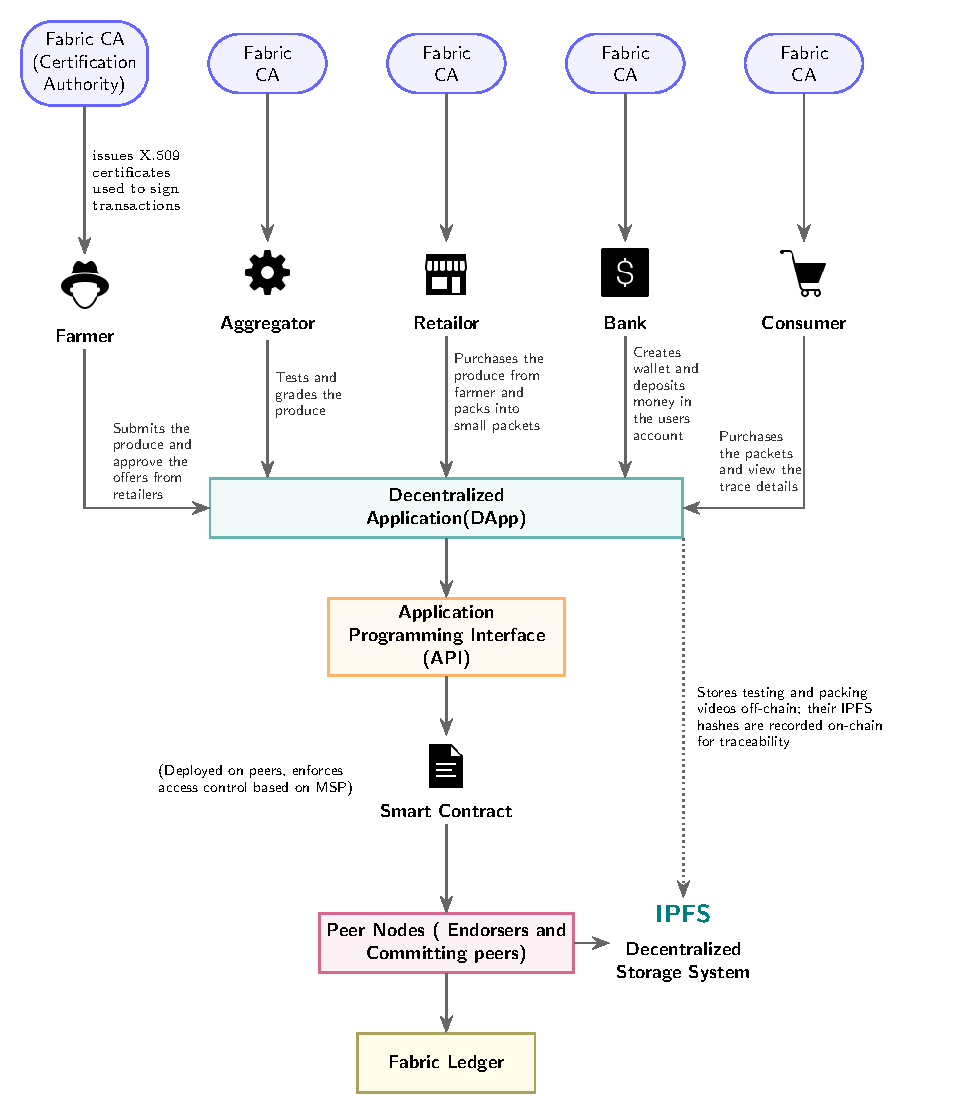
\includegraphics[width=0.9\textwidth]{Figure_1.pdf}
	\caption{System overview of the proposed agricultural supply chain platform}
	\label{fig:system_overview}
\end{figure}
	
	\subsection{Blockchain Network Architecture}
	
The blockchain network was implemented using Hyperledger Fabric with five organizations: FarmersMSP, AggregatorsMSP, RetailersMSP, ConsumersMSP, and BankMSP. Each organization was configured with its own peer, MSP, and certificate authority. The organizations interact through a common channel, while CouchDB stores the world state. The network was created by extending the Fabric test network using customized Docker Compose, crypto-configuration, and channel configuration files. Raft was used as the ordering mechanism. The detailed topology of these organizations and their respective peer nodes is presented in Figure \ref{fig:network_peer}.
	
	
	\begin{figure}[htbp]
		
		\centering
		
		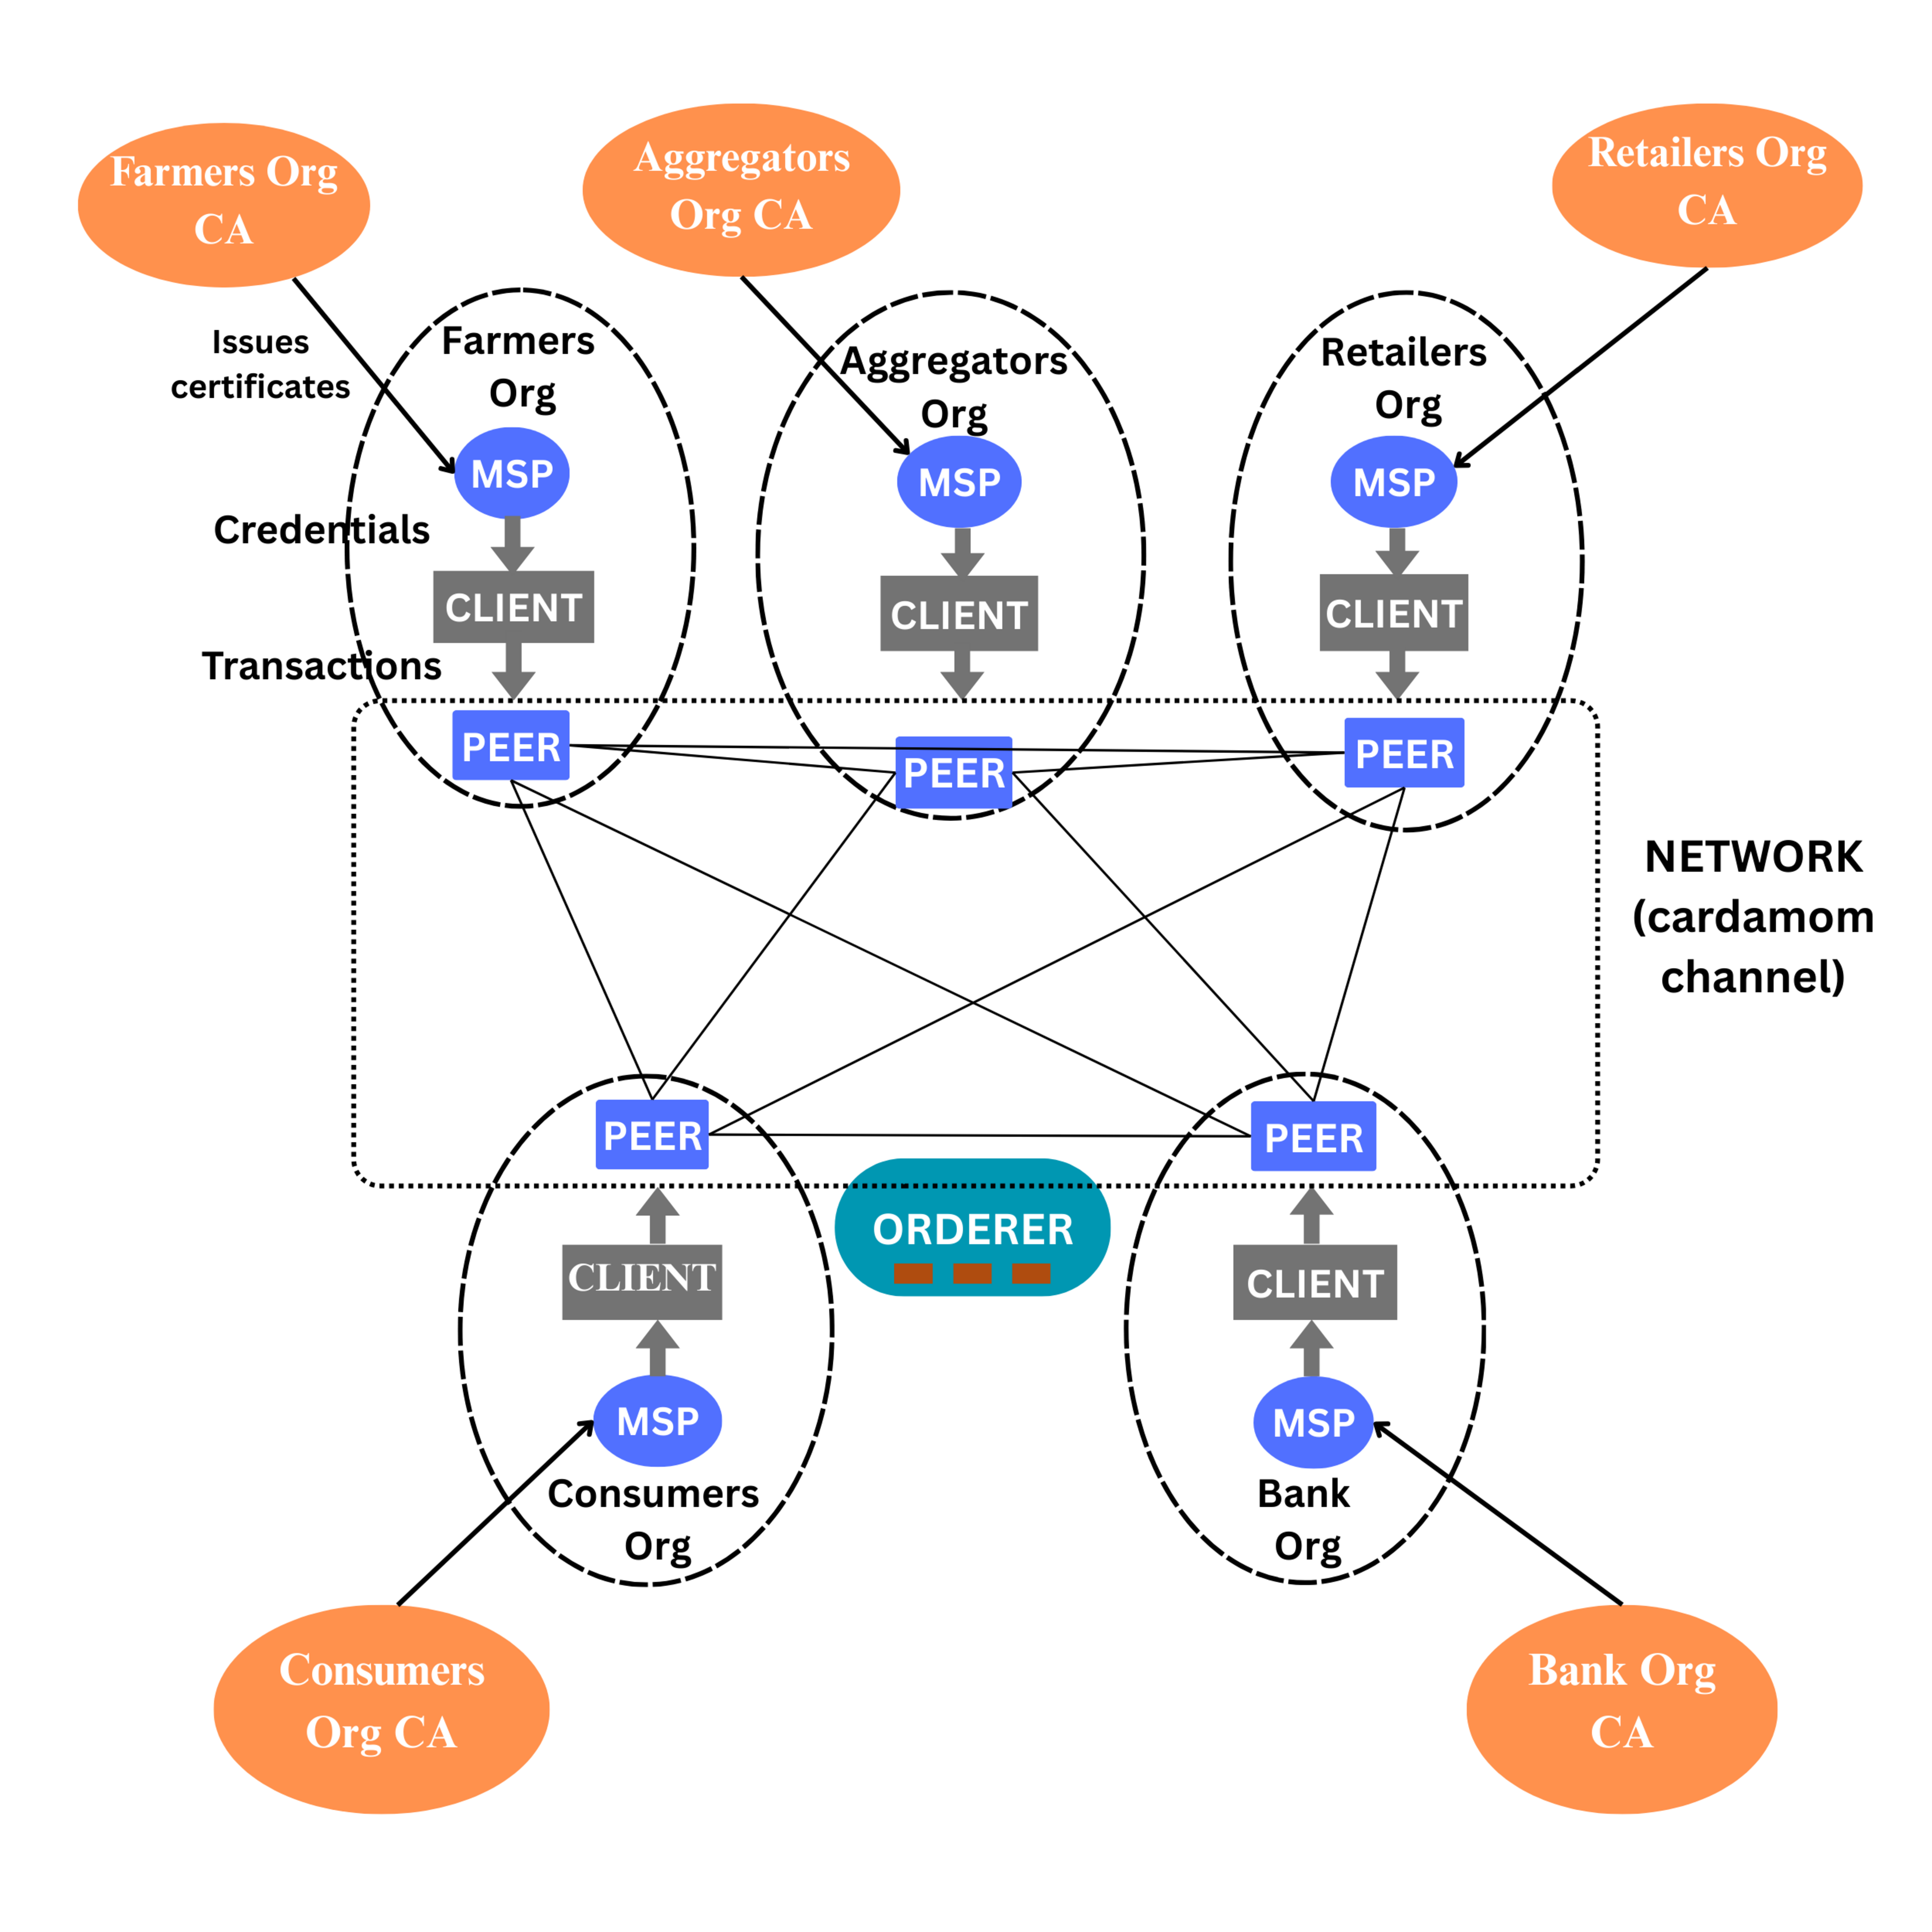
\includegraphics[width=\textwidth]{Figure_2.png}
		
		\caption{Blockchain network architecture of the proposed platform}
		
		\label{fig:network_peer}
		
	\end{figure}
	
	
\subsection{Smart Contract Workflow}

The business logic was implemented as JavaScript chaincode. The bank creates and funds wallets using \texttt{createAccount}. Farmers submit lots via \texttt{createLot}, and aggregators update quality status using \texttt{testCoffee}. Retailers bid via \texttt{makeOffer}, and the highest bidder executes \texttt{purchaseLot}, transferring funds automatically from their wallet to the farmer's wallet. Retailers repackage purchased lots using \texttt{createPacket}. Key features include: \texttt{createWallet()} and \texttt{depositMoney()}. Farmers submit agricultural lots using \texttt{submitProduce()}, and the testing fee is transferred to the selected aggregator. Aggregators record quality test results and grading details using \texttt{testCoffee()}. Approved lots are made available for retailer offers through \texttt{makeOffer()}, and farmers accept the highest valid offer using \texttt{acceptOffer()}. Retailers then pack accepted lots into packets using \texttt{packLotIntoPackets()}, while consumers purchase packets using \texttt{purchasePacket()} and verify provenance through lifecycle query functions. The overall sequence of stakeholder actions and smart contract functions is shown in Figure~\ref{fig:chaincode_flow}.

\begin{figure}[H]
	\centering
	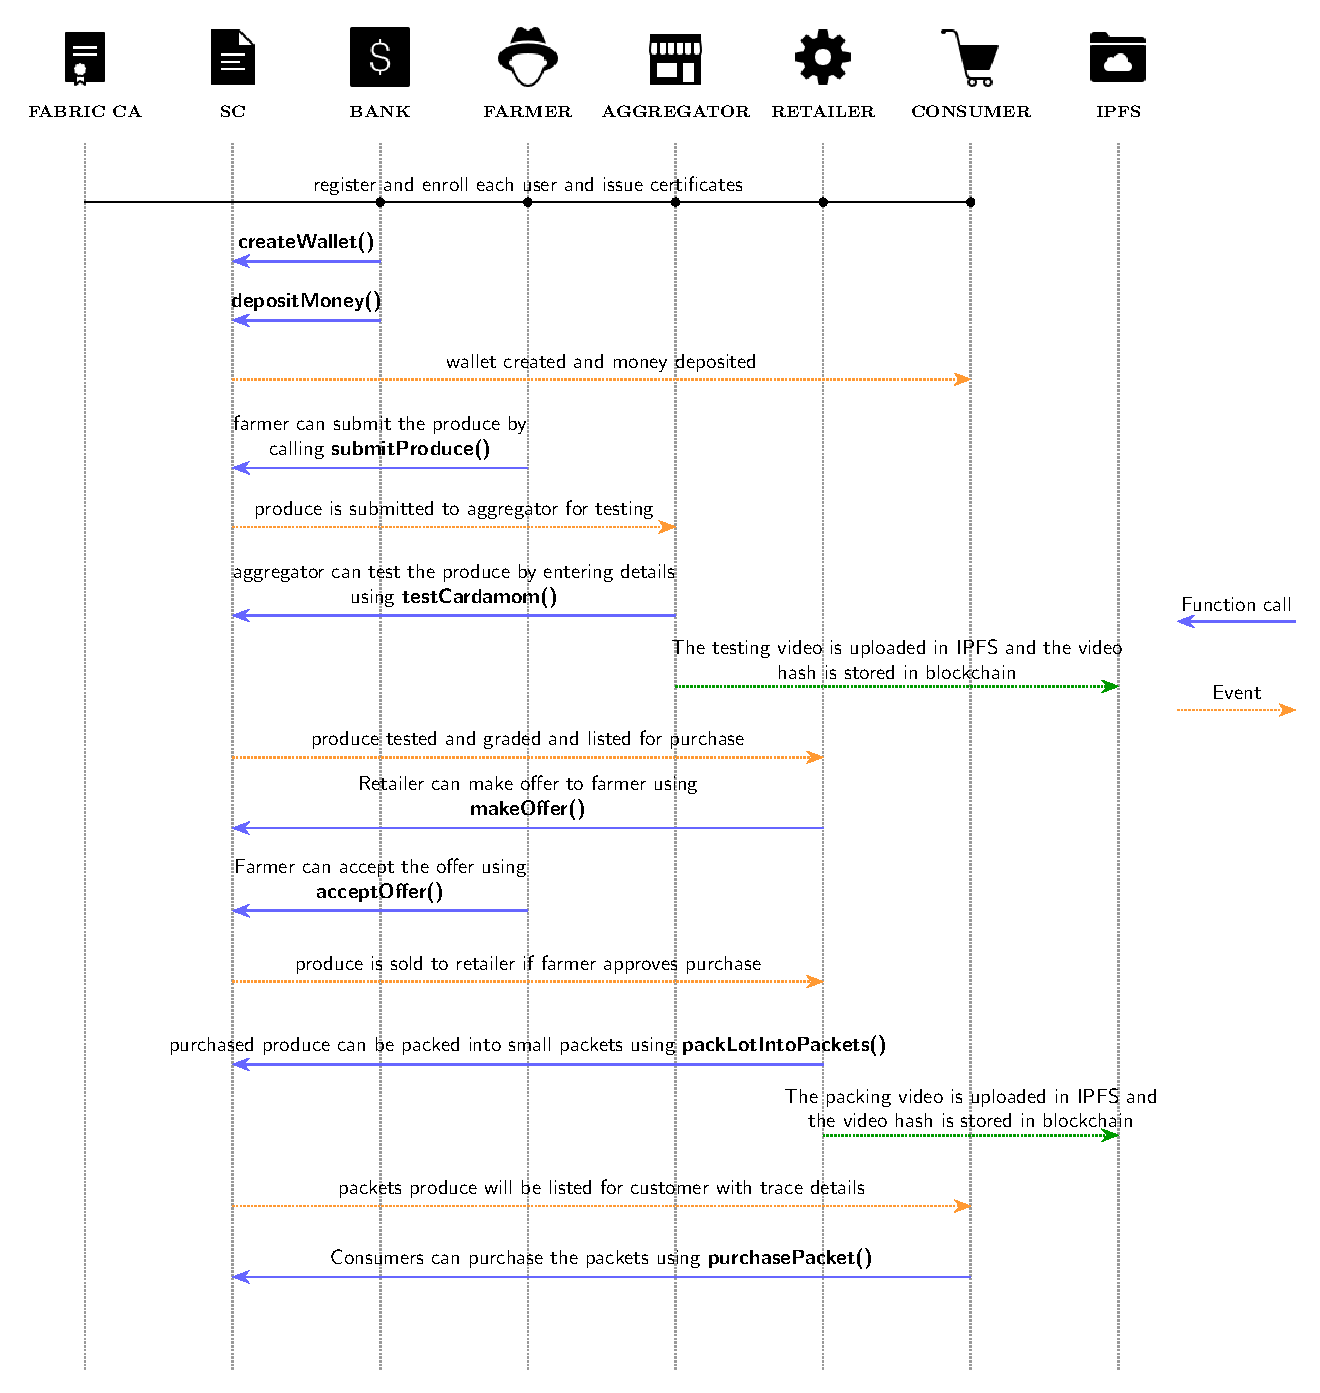
\includegraphics[width=\textwidth]{Figure_3.pdf}
	\caption{Smart Contract Execution Sequence and Stakeholder Interactions}
	\label{fig:chaincode_flow}
\end{figure}

\subsection{MVCC Conflict Vulnerabilities}

In high-throughput environments, the unoptimized chaincode is highly susceptible to Multi-Version Concurrency Control (MVCC) conflicts. Hyperledger Fabric employs an optimistic concurrency model: transactions are executed, endorsed, and ordered before validation against the ledger state. During the validation phase, if the version of a state key read during execution does not match the current committed version on the ledger, the transaction is marked invalid (MVCC \texttt{READ\_CONFLICT}) and abruptly dropped. In this supply chain design, there are two primary architectural bottlenecks where these conflicts predominantly occur:

\begin{enumerate}
    \item \textbf{Wallet Edits (\textit{submitProduce}, \textit{acceptOffer}, \textit{purchasePacket}):} Functions that facilitate financial transactions inherently invoke a shared internal \texttt{\_transfer} method. This method reads the current wallet balances of the sender and receiver, computes the new balances, and executes a \texttt{putState} operation to overwrite them. When multiple participants interact with a single entity concurrently (e.g., 50 farmers simultaneously submitting produce to a single aggregator), all 50 transactions read the exact same initial version of the aggregator's wallet key. The first transaction to successfully commit will increment the ledger version of that wallet. Consequently, the remaining 49 transactions will fail validation, severely throttling throughput.
    
    \item \textbf{Lot Highest Offer Edits (\textit{makeOffer}):} The auction mechanism allows multiple retailers to bid on an available agricultural lot concurrently. The \texttt{makeOffer} function reads the lot's current \texttt{highestOffer} parameter, validates if the new incoming bid is strictly greater, and overwrites the lot state. If multiple retailers bid on the exact same lot within the same block generation window, only the first endorsed transaction will successfully commit the updated lot state. The subsequent bids will encounter an MVCC conflict on the lot's shared composite key, causing those transactions to fail regardless of whether their bid values were objectively higher.
\end{enumerate}

These structural vulnerabilities form the foundational basis for the machine learning predictive models developed in this study, explicitly linking function complexity and hot-key density to deterministic transaction failure rates.


\section{Methodology}

To systematically evaluate and predict throughput and failure rates across multiple concurrent users and varying transaction loads, the experiment is conducted in three stages. First, a function-complexity analysis is performed to assess the functions evaluated based on ledger writes, ledger reads, and payload sizes. Second, an empirical analysis examines the variation in transaction throughput and failure rates across multiple factors, including transactions per second (tps), function complexity, concurrent participant density, and network latency. Third, having established the empirical relationships, the collected data is used to train machine learning models capable of predicting throughput and failures under varying network conditions. The study is further extended to identify the predominant features that influence the throughput and failure rate. 

\subsection{Function Complexity Analysis}

To precisely quantify the structural complexity of the functions in the chaincode, a custom static analysis pipeline (\textit{analyzeComplexity}) was developed. This tool parses the functions to extract operational metrics per function, including the total number of ledger reads (\textit{getState}), ledger writes (\textit{putState}), conditional branches, and iteration loops. Crucially, the tool explicitly identifies the exact composite keys targeted during write operations (MVCC Write Keys). By defining these structural metrics (detailed in Table \ref{tab:function_complexity}), the machine learning model can definitively correlate transaction performance with the exact number of highly contested hot-keys updated per invocation.
\begin{table}[ht]
\centering
\caption{Static Analysis of Smart Contract Function Complexity and MVCC Hot-Keys}
\label{tab:function_complexity}
\resizebox{\columnwidth}{!}{%
\begin{tabular}{|l|c|c|c|c|}
\hline
\textbf{Function} & \textbf{Payload (Bytes)} & \textbf{Total Reads} & \textbf{Total Writes} & \textbf{MVCC Write Keys} \\
\hline
\textit{submitProduce} & 64.72 & 3 & 3 & Wallet Balance (fromKey, toKey) \\ \hline
\textit{testCoffee} & 484.79 & 1 & 1 & None \\ \hline
\textit{makeOffer} & 40.65 & 2 & 1 & lot.highestOffer \\ \hline
\textit{acceptOffer} & 34.80 & 3 & 3 & Wallet Balance (fromKey, toKey) \\ \hline
\textit{packLotIntoPackets} & 90.77 & 1 & $1+n$ & None \\ \hline
\textit{purchasePacket} & 41.60 & 3 & 3 & Wallet Balance (fromKey, toKey) \\
\hline
\end{tabular}%
}
\end{table}

\vspace{0.2cm}
\noindent \small{*Note: For the empirical benchmarking simulations conducted in this study, the number of packets generated per lot ($n$) during the \textit{packLotIntoPackets} function was fixed at 55.}

 
  \subsubsection{Mechanics of MVCC Hot-Key Contention}
  In Hyperledger Fabric, MVCC conflicts occur when the same key is attempted to be written by multiple transactions simultaneously. The primary reason for these conflicts is the delay between transaction endorsement and final commitment in Hyperledger Fabric, during which the ordering service sequences transactions into blocks before they are validated and committed to the ledger. Preventing concurrent writes to ledger keys ensures data integrity. However, transactions involving these hot keys often encounter multiple failures, particularly at high transaction speeds.

\subsection{Empirical Benchmarking Setup}



The performance of the blockchain network was evaluated using Hyperledger Caliper. The primary objective is to study the variation in transaction throughput and failure rate in response to multiple factors, including transaction load (tps), concurrent hot-key participant density, network latency, and function complexity. The following sections describe the selected ranges of experimental factors.

\subsubsection{Transaction Loads and Workload Functions}
To capture the full spectrum of system performance, the experiments were conducted across a sequence of fixed-rate Transaction Per Second (TPS) loads: 1, 2, 4, 8, 10, 20, 50, 100, 200, 400, and 500 TPS. The benchmarking suite tested multiple distinct chaincode functions, including \textit{testCoffee}, \textit{makeoffer}, \textit{acceptoffer}, \textit{pack}, and \textit{submitproduce}. Each of these functions possesses a different structural complexity in terms of the number of state reads and writes required, as well as the number of participants contending for the same ledger key. Table \ref{tab:workload_functions_summary} summarizes the specific TPS ranges and latency configurations applied to each function during the empirical testing phase.

\begin{table}[H]
\centering
\caption{Summary of Workload Functions and Empirical Testing Parameters}
\label{tab:workload_functions_summary}
\resizebox{\columnwidth}{!}{%
\begin{tabular}{|l|p{0.55\linewidth}|p{0.25\linewidth}|}
\hline
\textbf{Workload Function} & \textbf{Transaction Send Rate (TPS) Ranges} & \textbf{Network Latency (ms)} \\
\hline
\textit{submitProduce()} & 1, 2, 4, 8, 10, 20, 50, 100, 200, 400, 500 & 0, 25, 50, 100 \\
\hline
\textit{makeOffer()} & 1, 2, 4, 8, 10, 20, 50, 100, 200, 400, 500 & 0, 25, 50, 100 \\
\hline
\textit{acceptOffer()} & 1, 2, 4, 8, 10, 20, 50, 100, 200, 400, 500 & 0, 25, 50, 100 \\
\hline
\textit{purchasePacket()} & 1, 2, 4, 8, 10, 20, 50, 100, 200, 400, 500 & 0, 25, 50, 100 \\
\hline
\textit{packLotIntoPackets()} & 1, 2, 4, 8, 10, 20, 50, 100, 200, 400, 500 & 0, 25, 50, 100 \\
\hline
\textit{testCoffee()} & 1, 2, 4, 8, 10, 20, 50, 100, 200, 400, 500 & 0, 25, 50, 100 \\
\hline
\end{tabular}%
}
\end{table}

\subsubsection{How Ledger Writes are Scaled in the Pack Function}
To explicitly isolate and study the performance impact of ledger write complexity, a targeted empirical study was conducted using the \textit{pack} function. By systematically varying the number of output packets created during a single transaction, the number of sequential ledger writes (\texttt{putState}) was dynamically scaled without introducing additional MVCC participant contention. Table \ref{tab:pack_ledger_writes} outlines the precise mathematical scaling of ledger writes as the target lot size increases. The findings of this write-complexity study are discussed comprehensively in the Results section.
\begin{table}[H]
\centering
\caption{Ledger Write Complexity Scaling based on Target Lot Size}
\label{tab:pack_ledger_writes}
\resizebox{0.75\columnwidth}{!}{%
\begin{tabular}{|l|c|}
\hline
\textbf{Target Lot Configuration} & \textbf{Sequential Ledger Writes (\texttt{putState})} \\
\hline
10kg Lot (\textit{pack\_r5}) & 58 \\
\hline
20kg Lot (\textit{pack20kg\_r5}) & 115 \\
\hline
50kg Lot (\textit{pack50kg\_r5}) & 286 \\
\hline
100kg Lot (\textit{pack100kg\_r5}) & 571 \\
\hline
\end{tabular}%
}
\end{table}

\subsubsection{Network Latency Simulation}
The methodology incorporated a network latency study to assess the system performance in real deployments by injecting artificial latency during the benchmarking phase. The latency simulations were conducted at specific thresholds: a baseline of 0 ms (representing an idealized, localized network), as well as  25 ms, 50 ms, 100 ms, and 200 ms. These configurations were specifically applied to observe the compounding impact of network delays on throughput ceilings and transaction failure rates. All the benchmarking experiments were conducted separately at each of these latencies.

\subsubsection{Strategic Participant Matrix and Dynamic Caliper Network Generation}

To evaluate the impact of concurrent user scaling without exhaustively testing redundant participant combinations, a strategic participant matrix was designed. The number of participants for key roles (e.g., Farmers, Aggregators, Retailers) was scaled across predefined thresholds: 1, 2, 5, 10, 15, 20, and 24. 

For functions requiring multiple participants (such as Farmers submitting produce to Aggregators), a two-dimensional participant matrix was generated. As explained in Table \ref{tab:function_complexity}, functions including \textit{submitProduce}, \textit{acceptOffer}, and \textit{purchasePacket} involve two participant roles and possess two target hot-keys. By varying the participant range as shown in Table \ref{tab:workload_mapping}, the experiments capture a range of concurrent hot-key participants from 2 to 48. In the case of the \textit{makeOffer} function, it targets one lot hot-key, and depending on the number of retailers bidding on the selected lots, the total hot-key participants range from 1 to 50, as detailed in Table \ref{tab:workload_mapping}.
Caliper workers were dynamically allocated based on the specific workload parameters. For example, in a \textit{submitproduce} workload configured with 5 farmers and 5 aggregators (\textit{submitproduce\_f5\_a5}), Caliper explicitly spawned 5 parallel worker processes acting as independent farmers. During execution, each farmer process probabilistically targeted one of the 5 available aggregators, inducing MVCC conflicts on the specific aggregator hot-keys.

\begin{table}[ht]
\centering
\caption{Benchmark Workload Configurations and Participant Mapping}
\label{tab:workload_mapping}
\resizebox{\columnwidth}{!}{%
\begin{tabular}{|l|l|p{0.3\linewidth}|p{0.25\linewidth}|}
\hline
\textbf{Workload Function} & \textbf{Participant Roles} & \textbf{Participant Matrix Evaluated} & \textbf{Total Hot-Key Participants} \\
\hline
\textit{submitProduce} & Farmers, Aggregators & Evaluated as $(X,Y)$ pairs: (1,1), (2,2), (5,5), etc. & $X + Y$ \\
\hline
\textit{makeOffer} & Retailers, Target Lots & Retailers ($R$) and Target Lots ($L$) varied &  $L$  \\
\hline
\textit{acceptOffer} & Farmers, Retailers & Evaluated as $(X,Y)$ pairs: (1,1), (2,2), (5,5), etc. & $X + Y$ \\
\hline
\textit{purchasePacket} & Consumers, Retailers & Evaluated as $(X,Y)$ pairs: (1,1), (2,2), (5,5), etc. & $X + Y$ \\
\hline
\end{tabular}%
}
\end{table}


\subsection{Data Collection and Feature Extraction}

The empirical output logs generated by Hyperledger Caliper across all benchmarking permutations were consolidated and extracted to formulate the primary dataset for the machine learning pipeline.
  
  \subsubsection{Feature Selection and Extraction}
To capture the nonlinear interactions inherent in this blockchain architecture, the dataset's independent features were carefully selected and extracted to quantify both the dynamic computational load and the static state-write dependencies. The primary extracted features are summarized in Table \ref{tab:feature_selection}, which details the rationale behind tracking each variable:
  \begin{table}[H]
\centering
\caption{Selected Features for Machine Learning Prediction}
\label{tab:feature_selection}
\resizebox{\columnwidth}{!}{%
\begin{tabular}{|p{0.25\linewidth}|p{0.7\linewidth}|}
\hline
\textbf{Feature} & \textbf{Description \& Rationale} \\
\hline
\textbf{Transaction Send Rate (Load)} & The targeted number of transactions submitted per second. \\
\hline
\textbf{Number of Caliper Workers} & The number of parallel client workers actively submitting transactions simultaneously, directly dictating concurrent thread pressure. \\
\hline

\textbf{Number of Ledger Writes} & Extracted via static analysis, representing baseline structural complexity. Allows mathematical correlation of algorithmic topology to failure vulnerabilities rather than relying on categorical function names. \\
\hline
\textbf{Hot-Key Participant Count} & A derived metric quantifying severity of concurrent operations on shared state keys (e.g., competing retailers bidding on a single lot, or simultaneous wallet balance edits during settlements). The total count of participants interacting with these precise hot-keys directly mathematically dictates the probability of an MVCC read-write conflict and transaction failure. \\
\hline
\textbf{Network Latency} & Injected artificial delay representing geographically distributed deployments. This feature dictates consensus overhead and exposes extended time windows where transactions are vulnerable to concurrent state changes during the validation phase. \\
\hline
\end{tabular}%
}
\end{table}

To provide a comprehensive dataset for the machine learning model, the benchmarking framework generated permutations across these features using the parameter ranges defined in Table \ref{tab:experimental_ranges}.

\begin{table}[H]
\centering
\caption{Experimental Benchmarking Parameter Ranges}
\label{tab:experimental_ranges}
\resizebox{\columnwidth}{!}{%
\begin{tabular}{|l|l|}
\hline
\textbf{Experimental Parameter} & \textbf{Evaluated Range / Values} \\
\hline
Transaction Send Rate (TPS) & 1, 2, 4, 8, 10, 20, 50, 100, 200, 400, 500 \\
Number of Caliper Workers & 1, 2, 5, 10, 15, 20, 24 \\
Participant Density Matrix & Symmetrical Pairs e.g., (1,1), (2,2), (4,4), (5,5), ... up to (24,24) \\
Transactions per Round & Dynamic (Calculated as Target TPS $\times$ Workload Duration) \\
Workload Duration & Fixed per permutation (e.g., 100 seconds) \\

\hline
\end{tabular}%
}
\end{table}

\begin{table}[H]
\centering
\caption{Fixed Network and Configuration Parameters}
\label{tab:fixed_parameters}
\resizebox{\columnwidth}{!}{%
\begin{tabular}{|l|l|}
\hline
\textbf{Configuration Parameter} & \textbf{Fixed Value} \\
\hline
Number of Caliper Workers & 5 \\
Block Size (BatchSize) & 100 Transactions \\
Block Timeout (BatchTimeout) & 2 Seconds \\
Consensus Mechanism & Raft Ordering Service \\
Endorsement Policy & Majority Endorsement \\
Peer Infrastructure & Identical Resource Allocation per Node \\
\hline
\end{tabular}%
}
\end{table}


\begin{table}[H]
\centering
\caption{Concurrent Hot-Key Contention Scaling Matrix across Participant Densities}
\label{tab:hotkey_scaling}
\begin{tabular}{|p{0.22\linewidth}|p{0.22\linewidth}|p{0.22\linewidth}|p{0.22\linewidth}|}
\hline
\textbf{\textit{submitProduce} Hot-Keys} & \textbf{\textit{makeOffer} Hot-Keys} & \textbf{\textit{acceptOffer} Hot-Keys} & \textbf{\textit{purchasePacket} Hot-Keys} \\
\hline
2 (1 Farmer, 1 Aggregator) & 1 Lot (1 Retailer competing) & 2 (1 Farmer, 1 Retailer) & 2 (1 Consumer, 1 Retailer) \\ \hline
8 (4 Farmers, 4 Aggregators) & 1 Lot (4 Retailers competing) & 8 (4 Farmers, 4 Retailers) & 8 (4 Consumers, 4 Retailers) \\ \hline
20 (10 Farmers, 10 Aggregators) & 1 Lot (10 Retailers competing) & 20 (10 Farmers, 10 Retailers) & 20 (10 Consumers, 10 Retailers) \\ \hline
30 (15 Farmers, 15 Aggregators) & 1 Lot (15 Retailers competing) & 30 (15 Farmers, 15 Retailers) & 30 (15 Consumers, 15 Retailers) \\ \hline
40 (20 Farmers, 20 Aggregators) & 1 Lot (20 Retailers competing) & 40 (20 Farmers, 20 Retailers) & 40 (20 Consumers, 20 Retailers) \\ \hline
48 (24 Farmers, 24 Aggregators)& 1 Lot (24 Retailers competing) & 48 (24 Farmers, 24 Retailers) & 48 (24 Consumers, 24 Retailers) \\
\hline
\end{tabular}
\end{table}

Table \ref{tab:experimental_ranges} details the specific benchmarking ranges traversed during the dataset generation phase, while the static infrastructure and configuration parameters held constant across all tests are detailed in Table \ref{tab:fixed_parameters}. Crucially, as the participant density scales, the mathematical severity of MVCC read-write conflicts scales accordingly. Table \ref{tab:hotkey_scaling} illustrates this concurrent hot-key contention scaling matrix across the evaluated participant densities for the core smart contract functions. For instance, in the \textit{submitProduce} function, scaling from 1 Farmer and 1 Aggregator up to 24 Farmers and 24 Aggregators drastically increases the number of concurrent updates targeting shared wallet state keys (from 2 concurrent hot-keys up to 48 concurrent hot-keys). By explicitly tracking this \textit{Hot-Key Participant Count} across all experimental rounds, the dataset captures the exact structural friction points that trigger blockchain transaction failures. The resulting consolidated dataset serves as the foundational empirical input for the predictive machine learning models.

\subsection{Predictive Modeling Framework}



\subsubsection{Evaluating Regression Architectures}
Predicting MVCC failures presents a unique mathematical challenge because blockchain performance degradation does not scale linearly. A network typically remains perfectly stable until a specific structural limit is hit (e.g., a critical mass of concurrent hot-key collisions or resource exhaustion), at which point performance drops off a severe "cliff" (jumping abruptly from 0\% to high failure rates). 

To determine the most accurate method for mapping these non-linear, multi-variable thresholds, three distinct machine learning regression architectures were initially evaluated, as outlined in Table \ref{tab:ml_models}:

\begin{table}[ht]
\centering
\caption{Evaluated Machine Learning Regression Architectures}
\label{tab:ml_models}
\resizebox{\columnwidth}{!}{%
\begin{tabular}{|p{0.3\linewidth}|p{0.2\linewidth}|p{0.5\linewidth}|}
\hline
\textbf{Predictive Model} & \textbf{Architecture Class} & \textbf{Description \& Rationale} \\
\hline
\textbf{Linear Regression} & Baseline & Linear baseline; tested to prove incapability of modeling discrete, non-linear MVCC state ceilings. \\
\hline
\textbf{Random Forest Regressor} & Tree Ensemble & Aggregates multiple independent decision trees to reduce prediction variance. \\
\hline
\textbf{Gradient Boosting} & Boosting Ensemble & Sequentially builds trees to explicitly correct residual errors; natively provides transparent feature importance extraction. \\
\hline
\end{tabular}%
}
\end{table}

The empirical evaluation of these models revealed stark differences in their capability to handle blockchain failure mechanics. As expected, linear mapping models like Linear Regression were fundamentally incapable of modeling the strict, sudden thresholds of MVCC failures. Conversely, tree-based ensemble methods successfully captured these dynamics. Tree algorithms inherently create distinct conditional splits (e.g., IF Hot-Keys $>$ 2 AND Load $>$ 300 $\rightarrow$ Failure = 85\%), perfectly mimicking the conditional transaction validation logic of blockchain state machines. 


Crucially, rather than predicting the absolute number of failed transactions (which is artificially biased by the total number of transactions sent), the models were trained to predict the precise \textit{Failure Rate} (the percentage of failed transactions over the total submitted), alongside the successfully achieved system \textit{Throughput}.



\section{Results and Discussion}
\subsection{Empirical Network Performance Analysis}
Each smart contract function was evaluated independently across a range of transaction send rates using Hyperledger Caliper. The functions assessed included \textit{submitProduce()}, \textit{testCoffee()}, \textit{makeOffer()}, \textit{acceptOffer()}, \textit{packLotIntoPackets()}, and \textit{purchasePacket()}. The objective of this phase was to establish a rigorous performance baseline for each function prior to the application of predictive modelling.

\subsubsection{Throughput Analysis: Testing with No Latency}
Figure \ref{fig:throughput-plot} illustrates the throughput response of each function under increasing transaction load. At lower send rates (50--100 TPS), most functions demonstrated steady, near-linear scaling. As the target load approached 500 TPS, however, significant performance divergence emerged across the function set. All baseline measurements in this phase were taken at 0 ms network latency with 10 Caliper workers. The structurally simplest function, \textit{makeOffer()}, achieved the highest sustained throughput, reaching a peak of 395.2 TPS. Functions with greater per-transaction write complexity, namely \textit{submitProduce()} and \textit{purchasePacket()}, reached saturation points of approximately 285.4 TPS and 305.2 TPS respectively. The \textit{acceptOffer()} function, evaluated at a participant density of 10, scaled comparably to the other write functions and attained 265.1 TPS at peak load. The \textit{packLotIntoPackets()} function exhibited the most constrained performance, with throughput capped at 132.2 TPS owing to the high number of sequential ledger writes executed per invocation. These results establish a consistent inverse relationship between per-transaction ledger write count and maximum achievable throughput.

\begin{figure}[H]
\centering
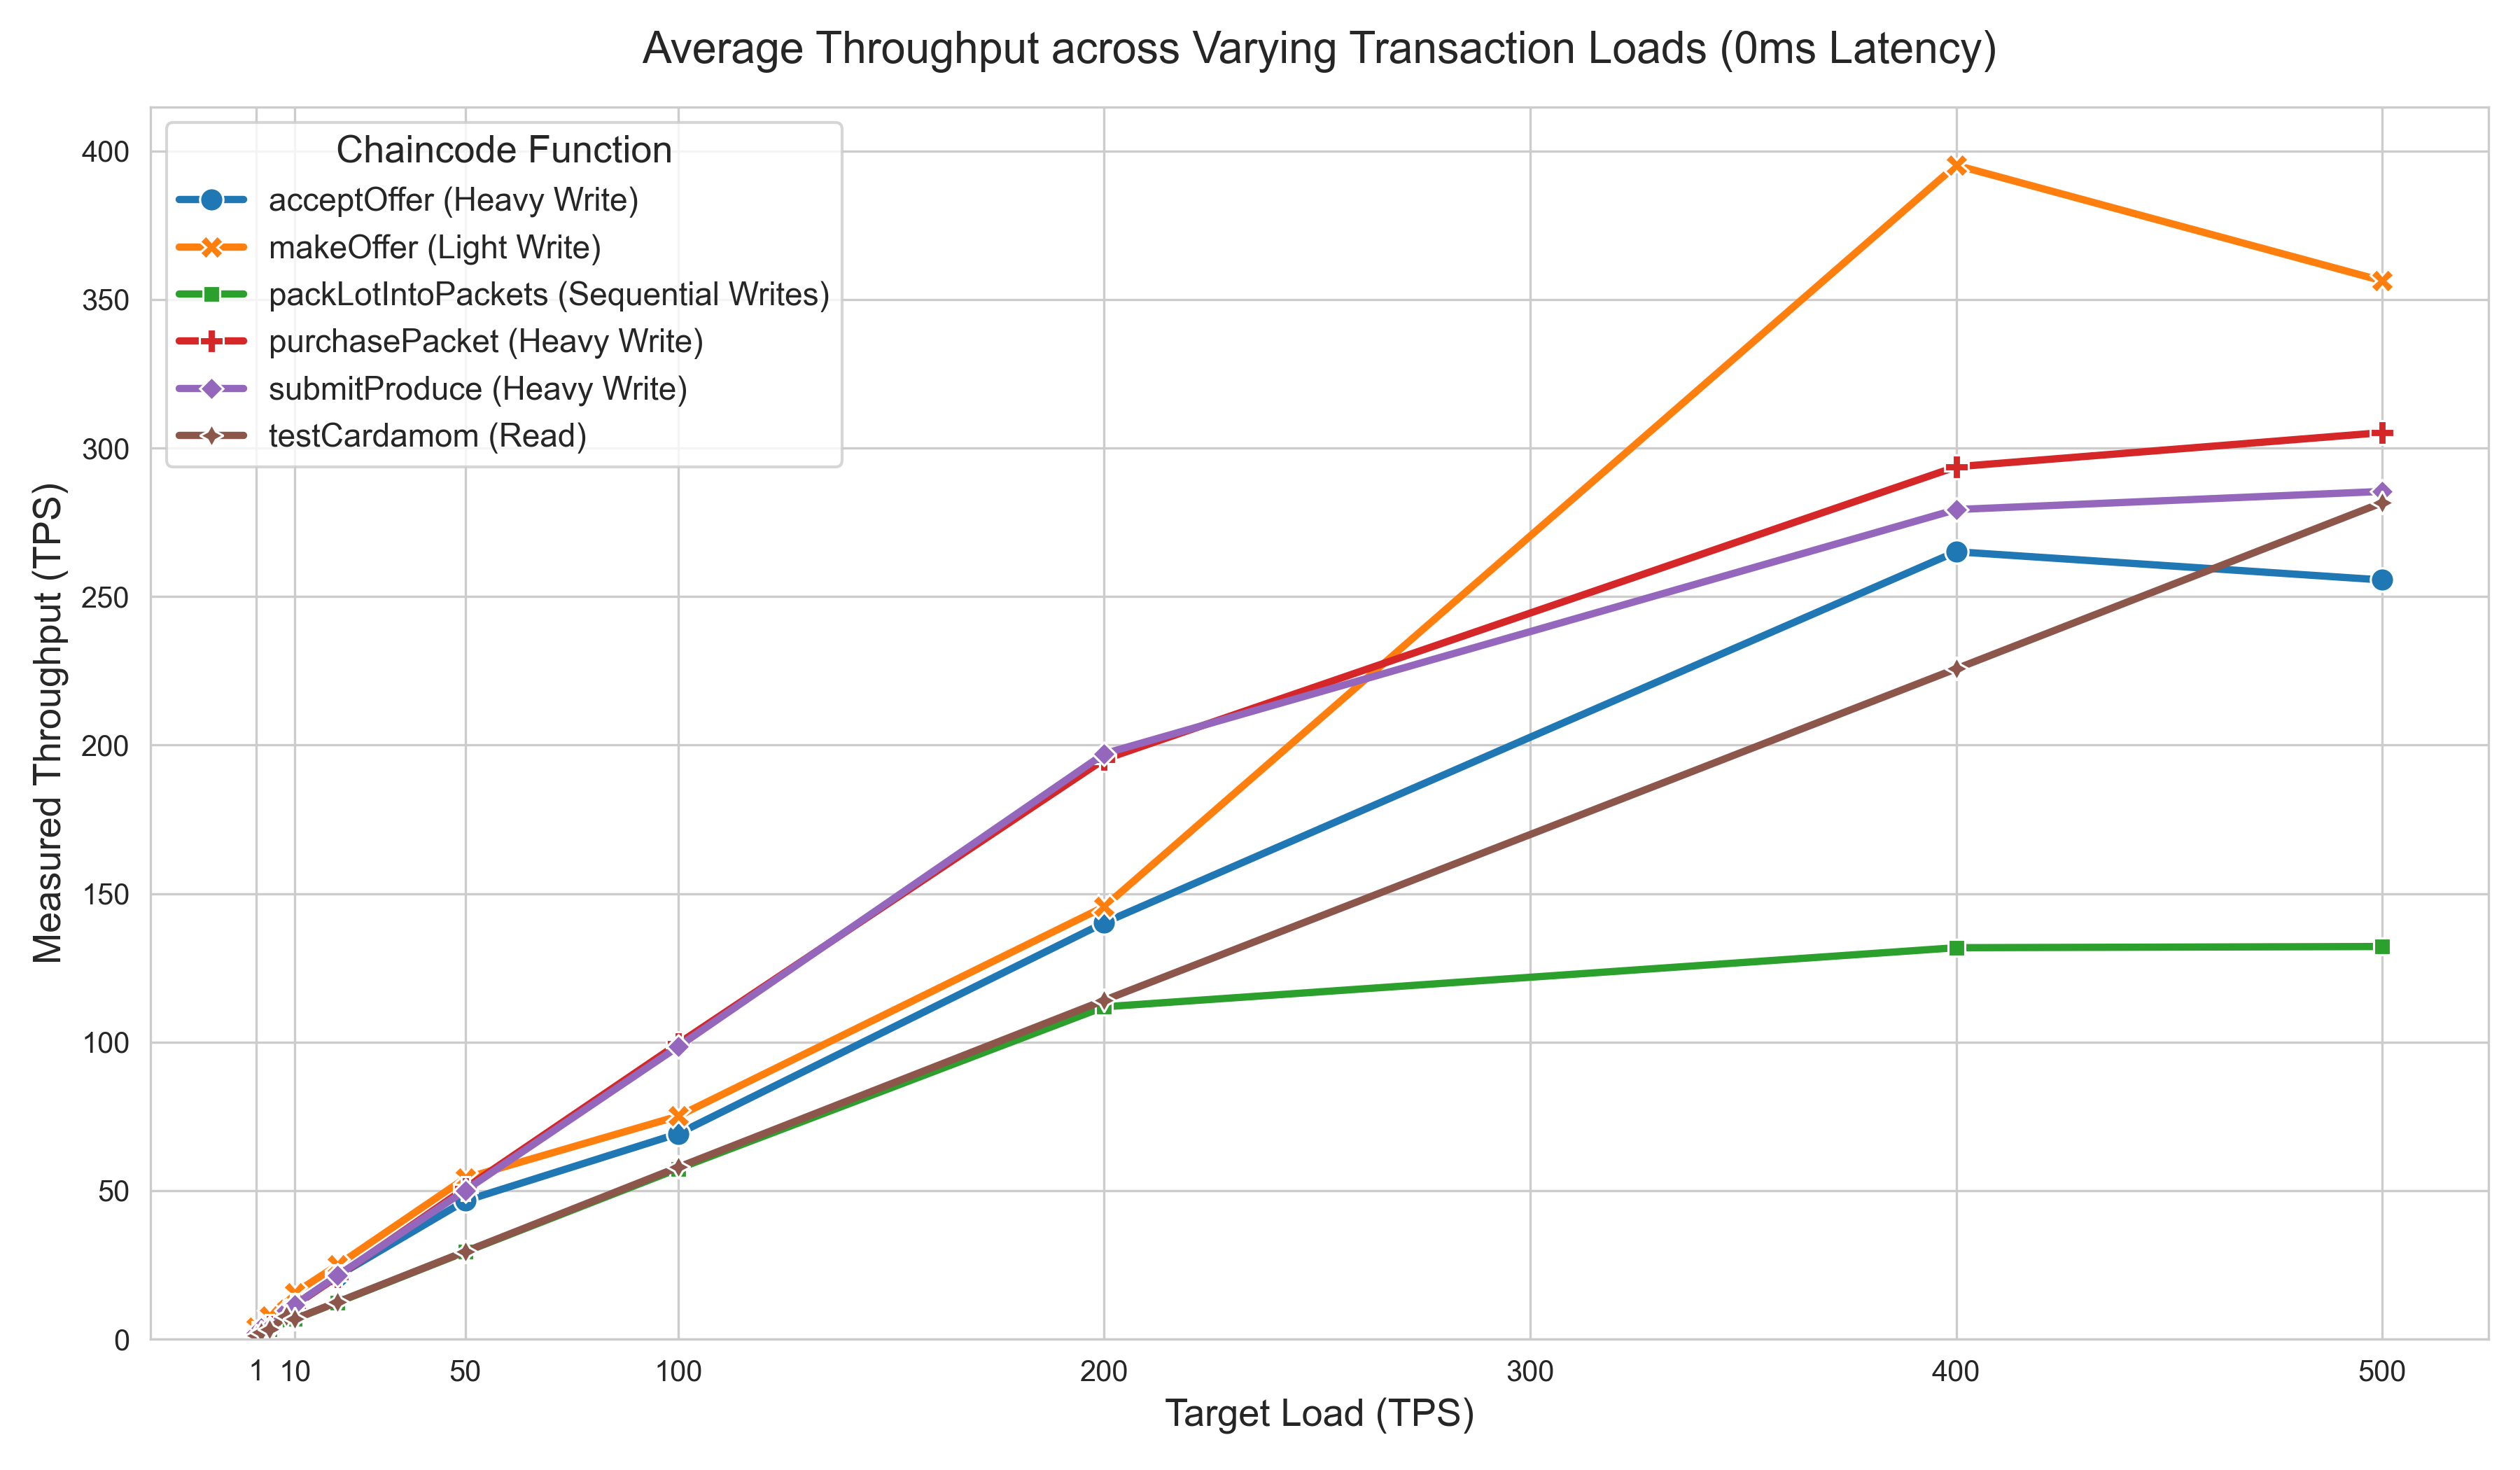
\includegraphics[width=0.8\textwidth]{Figure_4.png}
\caption{Average Throughput across varying transaction loads (evaluated at 0ms latency utilizing 10 Caliper workers).}
\label{fig:throughput-plot}
\end{figure}


\subsubsection{Throughput Analysis: Changing the Number of Writes}
Among the functions assessed, \textit{packLotIntoPackets()} exhibited the greatest sensitivity to ledger write volume, with throughput constrained to approximately 140 TPS irrespective of the target send rate.

Figures \ref{fig:throughput-pack-load-vs-throughput} and \ref{fig:throughput-degradation-200tps} provide a detailed examination of this relationship. Each invocation of \textit{packLotIntoPackets()} performs one write to update the parent lot record and one write per generated consumer packet. For a standard 10 kg lot, this yields approximately 59 ledger writes per transaction. For a 100 kg lot, the write count exceeds 572. Performance degradation scaled consistently with the number of writes, confirming that this bottleneck is attributable solely to the structural write complexity of the function and not to participant-level state contention.

The cumulative write load placed substantial strain on the endorsement and ordering pipeline, causing transaction latency to escalate at a rate disproportionate to that observed in structurally simpler functions.

\begin{figure}[H]
    \centering
    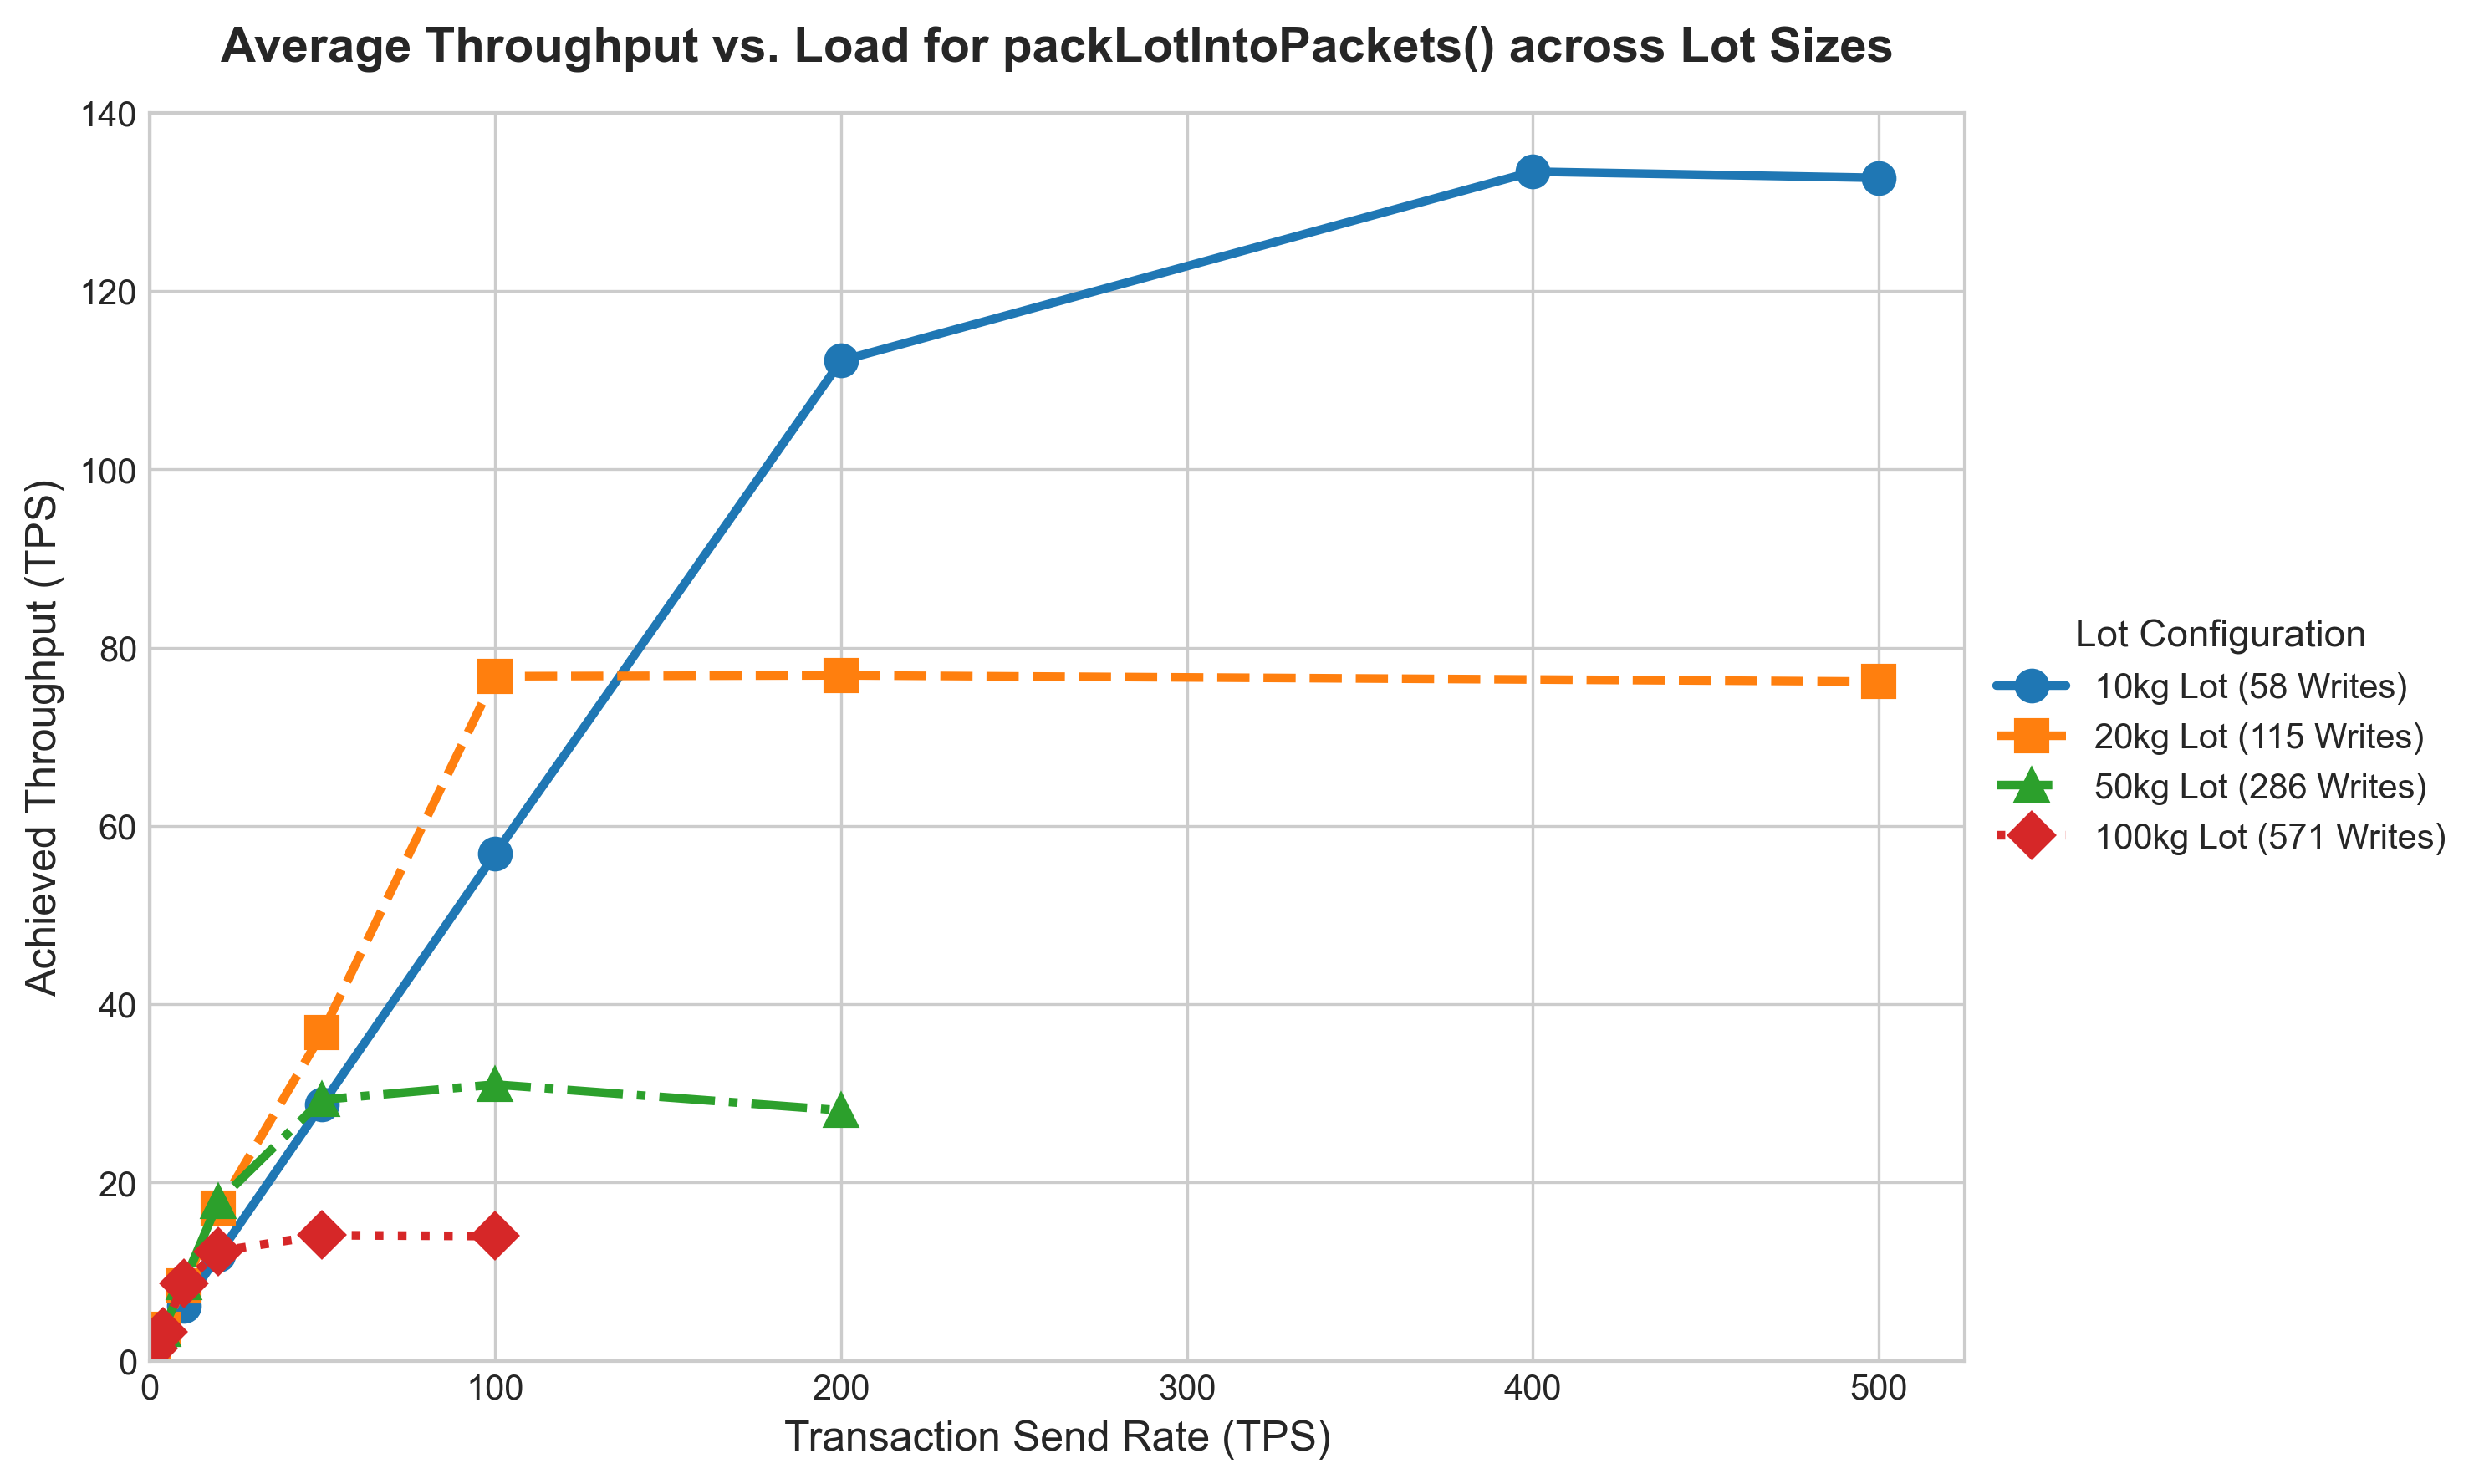
\includegraphics[width=0.8\textwidth]{Figure_5.png}
    \caption{Throughput vs Target Load (TPS) for Pack Functions across varying Ledger Writes (Lot Weights).}
    \label{fig:throughput-pack-load-vs-throughput}
\end{figure}

\begin{figure}[H]
    \centering
    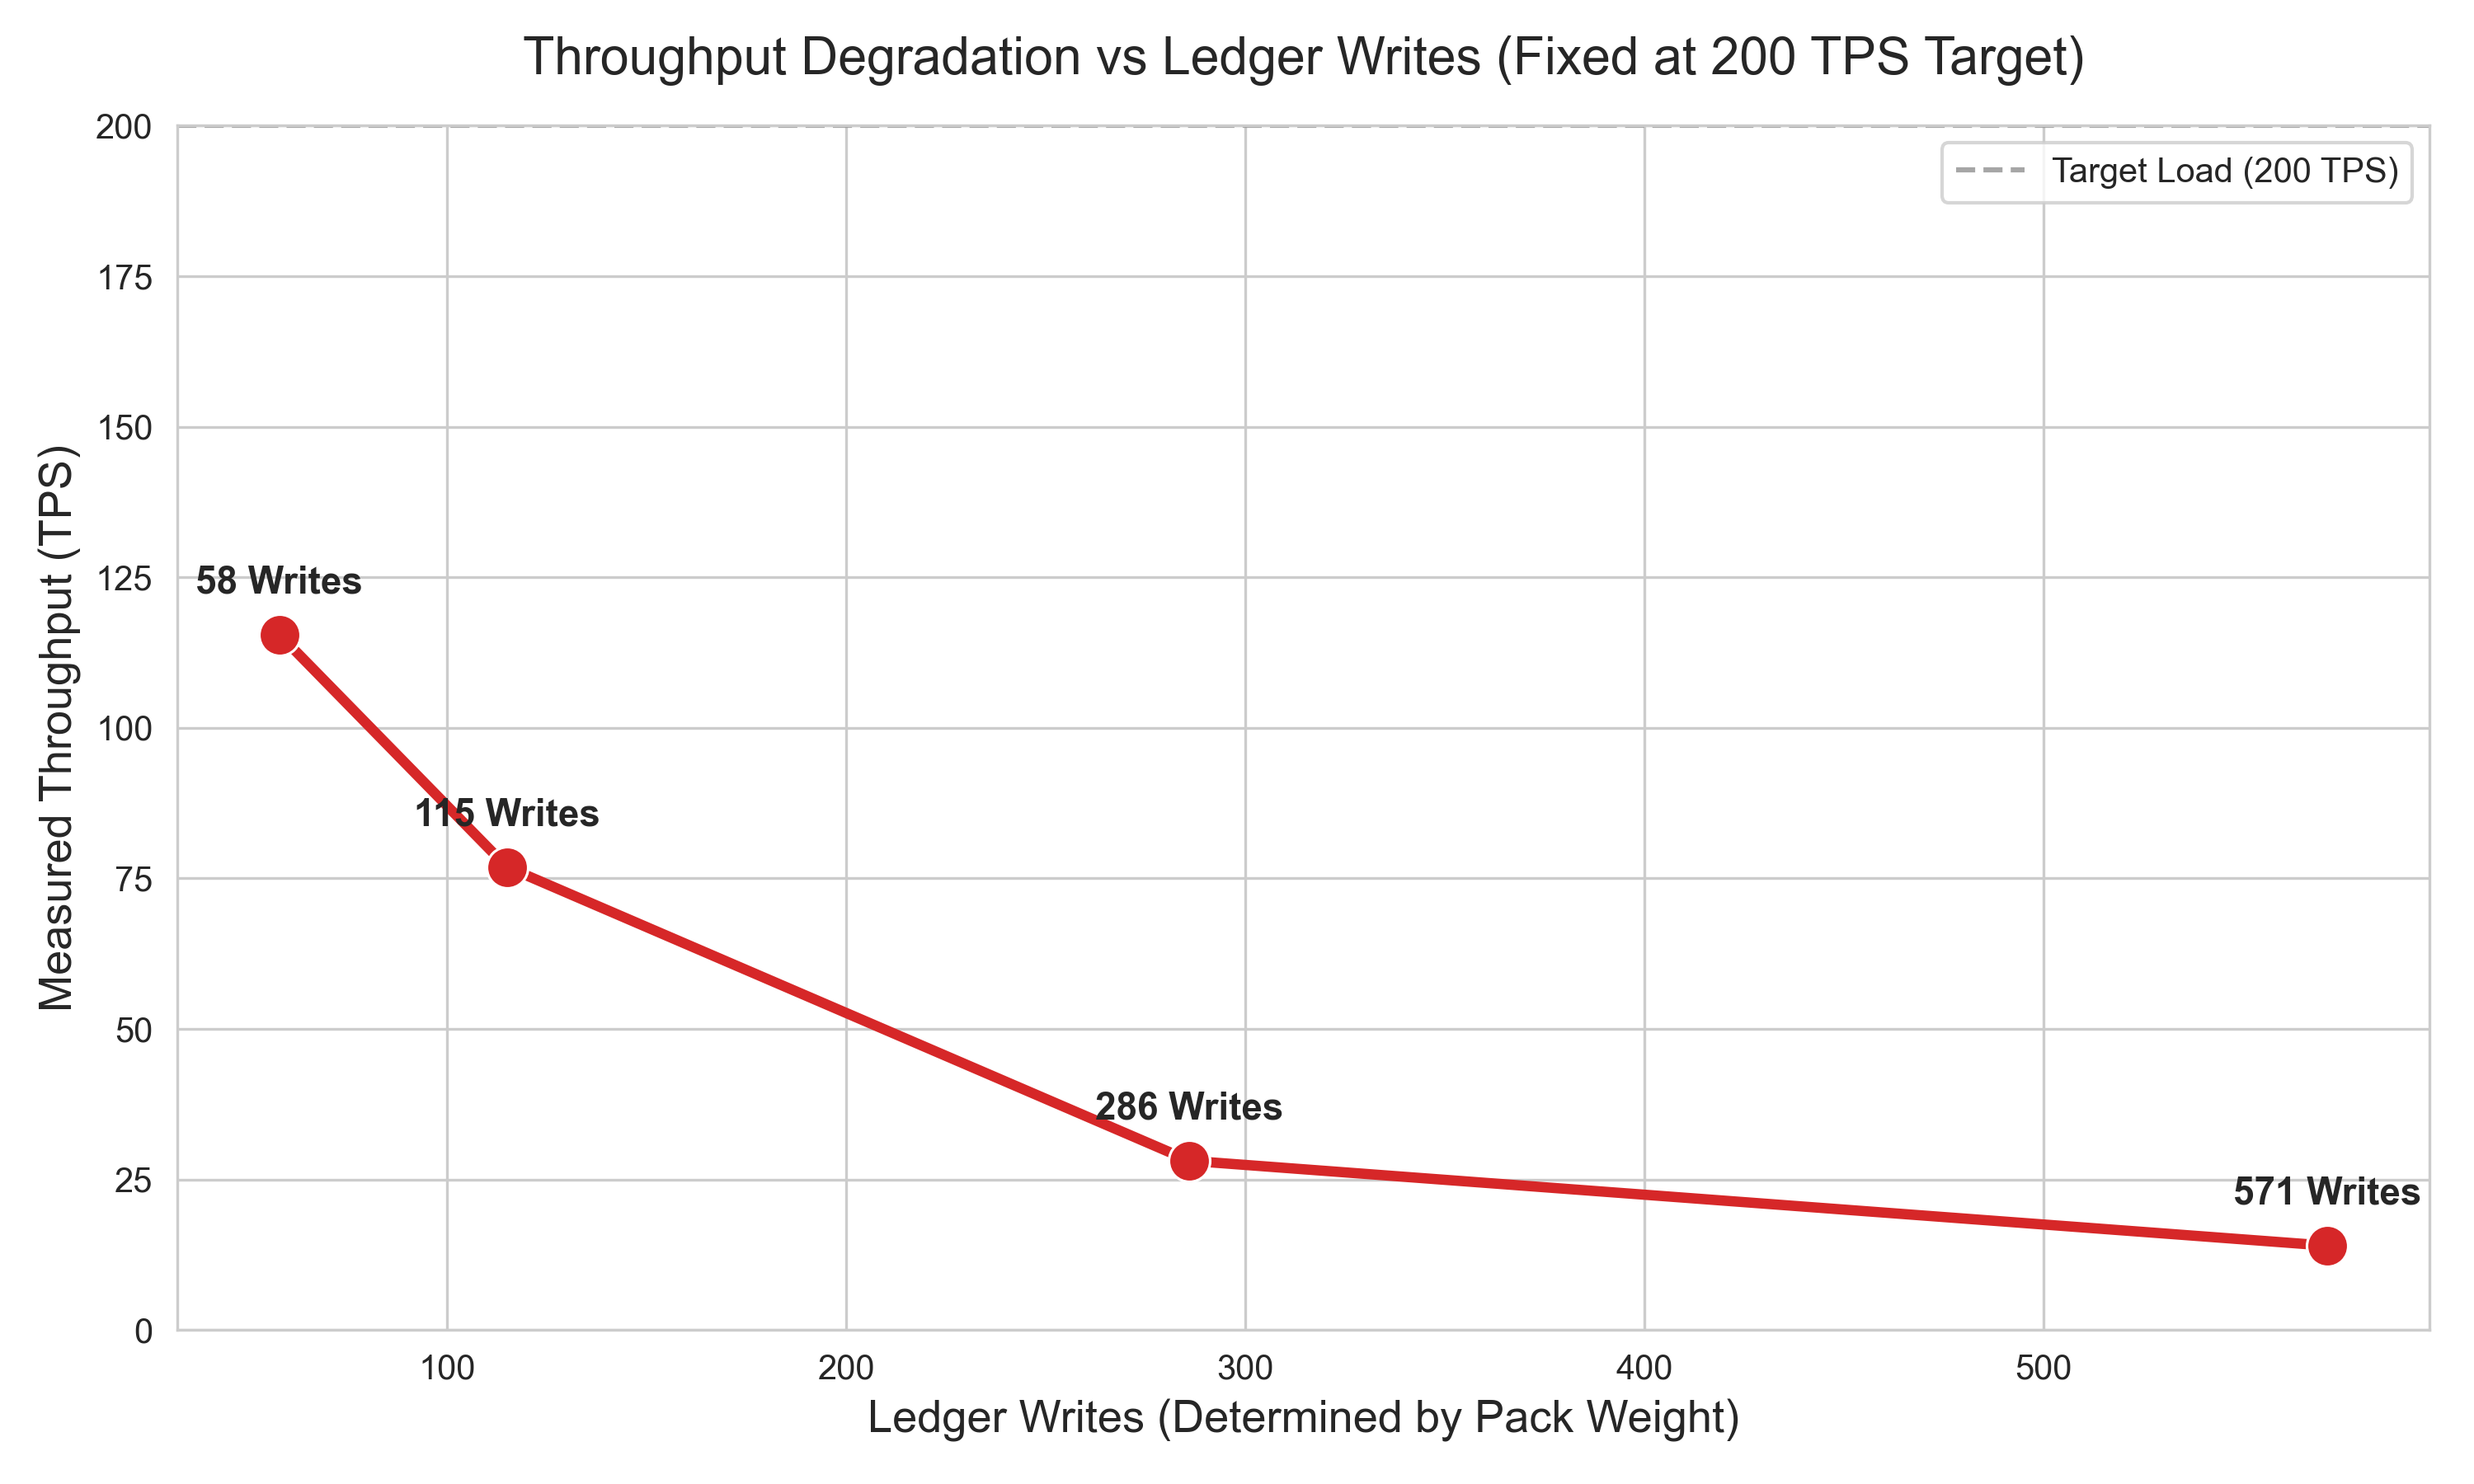
\includegraphics[width=0.8\textwidth]{Figure_6.png}
    \caption{Throughput Degradation at exactly 200 TPS Target Load across increasing Ledger Writes.}
    \label{fig:throughput-degradation-200tps}
\end{figure}

\subsubsection{Throughput Analysis: Introducing Network Latency}
To assess the impact of network conditions on throughput, artificial latency values ranging from 0 ms to 200 ms were injected into the Docker container interfaces using the Linux \texttt{netem} tool. Figure \ref{fig:pack_latency_200tps} presents the effect on \textit{packLotIntoPackets()} across the full range of target loads. A notable finding was that even a latency of 25 ms produced a substantial reduction in sustained throughput. In combination with the function's high write complexity, network delay accelerated performance degradation significantly, causing the system to fall short of its target load well before the theoretical maximum.
\begin{figure}[H]
\centering
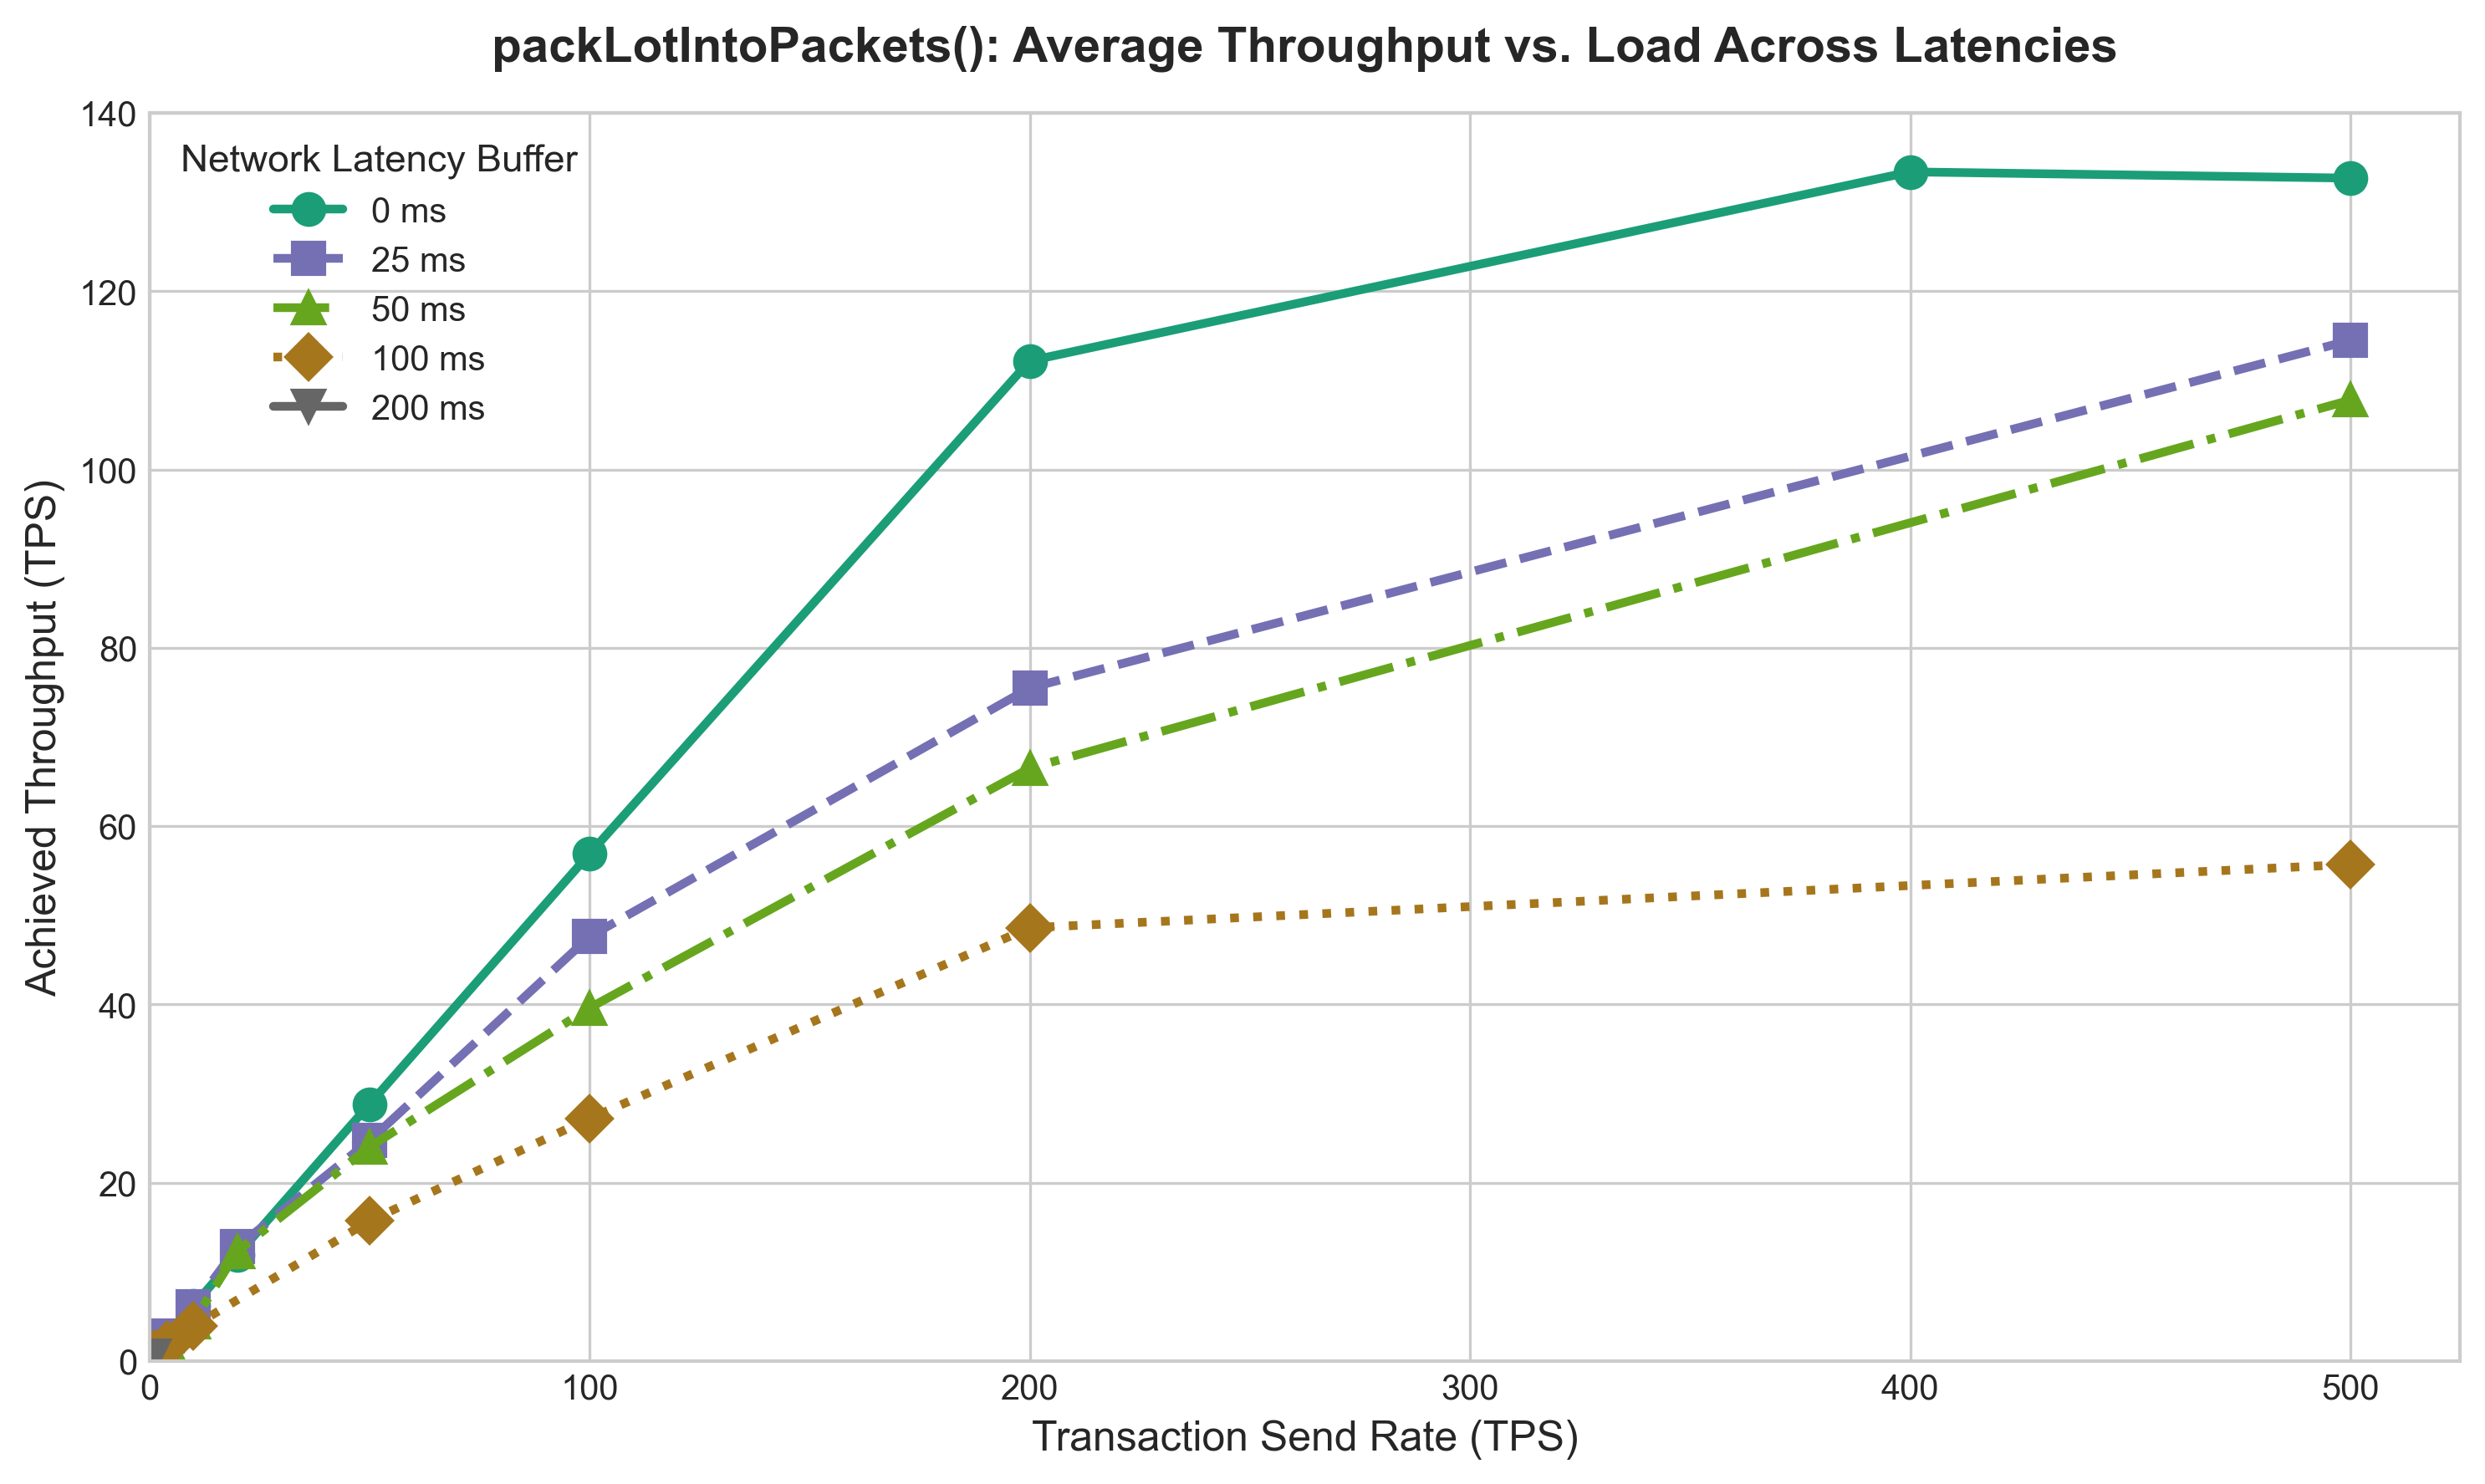
\includegraphics[width=0.8\textwidth]{Figure_7.png}
\caption{Performance of the \textit{packLotIntoPackets()} function across varying network latencies and target loads. The chart illustrates how sustained throughput collapses under severe sequential ledger write conditions as load and latency increase.}
\label{fig:pack_latency_200tps}
\end{figure}



\subsubsection{Failure Analysis without Latency}

To isolate the effect of participant-level state contention, network latency was fixed at 0 ms throughout this phase, thereby excluding transmission delay as a contributing variable.

As illustrated in Figure \ref{fig:hotkey_failures}, transaction failure rates exhibited a strong inverse relationship with the number of active participants. Under low participant densities, all concurrent transactions targeted the same small set of shared ledger records, producing a high rate of conflicting write operations. Hyperledger Fabric's MVCC validation layer rejected these conflicting transactions in large volumes, driving failure rates to critically high levels. As the participant count increased, the transaction workload was distributed across a broader set of independent ledger keys, substantially reducing the probability of concurrent write conflicts and lowering the observed failure rate.

\subsubsection{Failure Analysis with Latency}

Network latency was found to exacerbate participant-level contention considerably. As latency increases, transactions require more time to complete their endorsement and commit cycles. During this extended processing window, the ledger keys involved in each transaction remain subject to potential conflict with other in-flight transactions. The longer this window, the greater the likelihood that subsequently submitted transactions will encounter stale state versions, resulting in MVCC read conflicts and rejection. At elevated latency levels, failure rates approached 100\% even at moderate transaction send rates.

\begin{figure}[H]
    \centering
    \begin{minipage}[b]{0.48\textwidth}
        \centering
        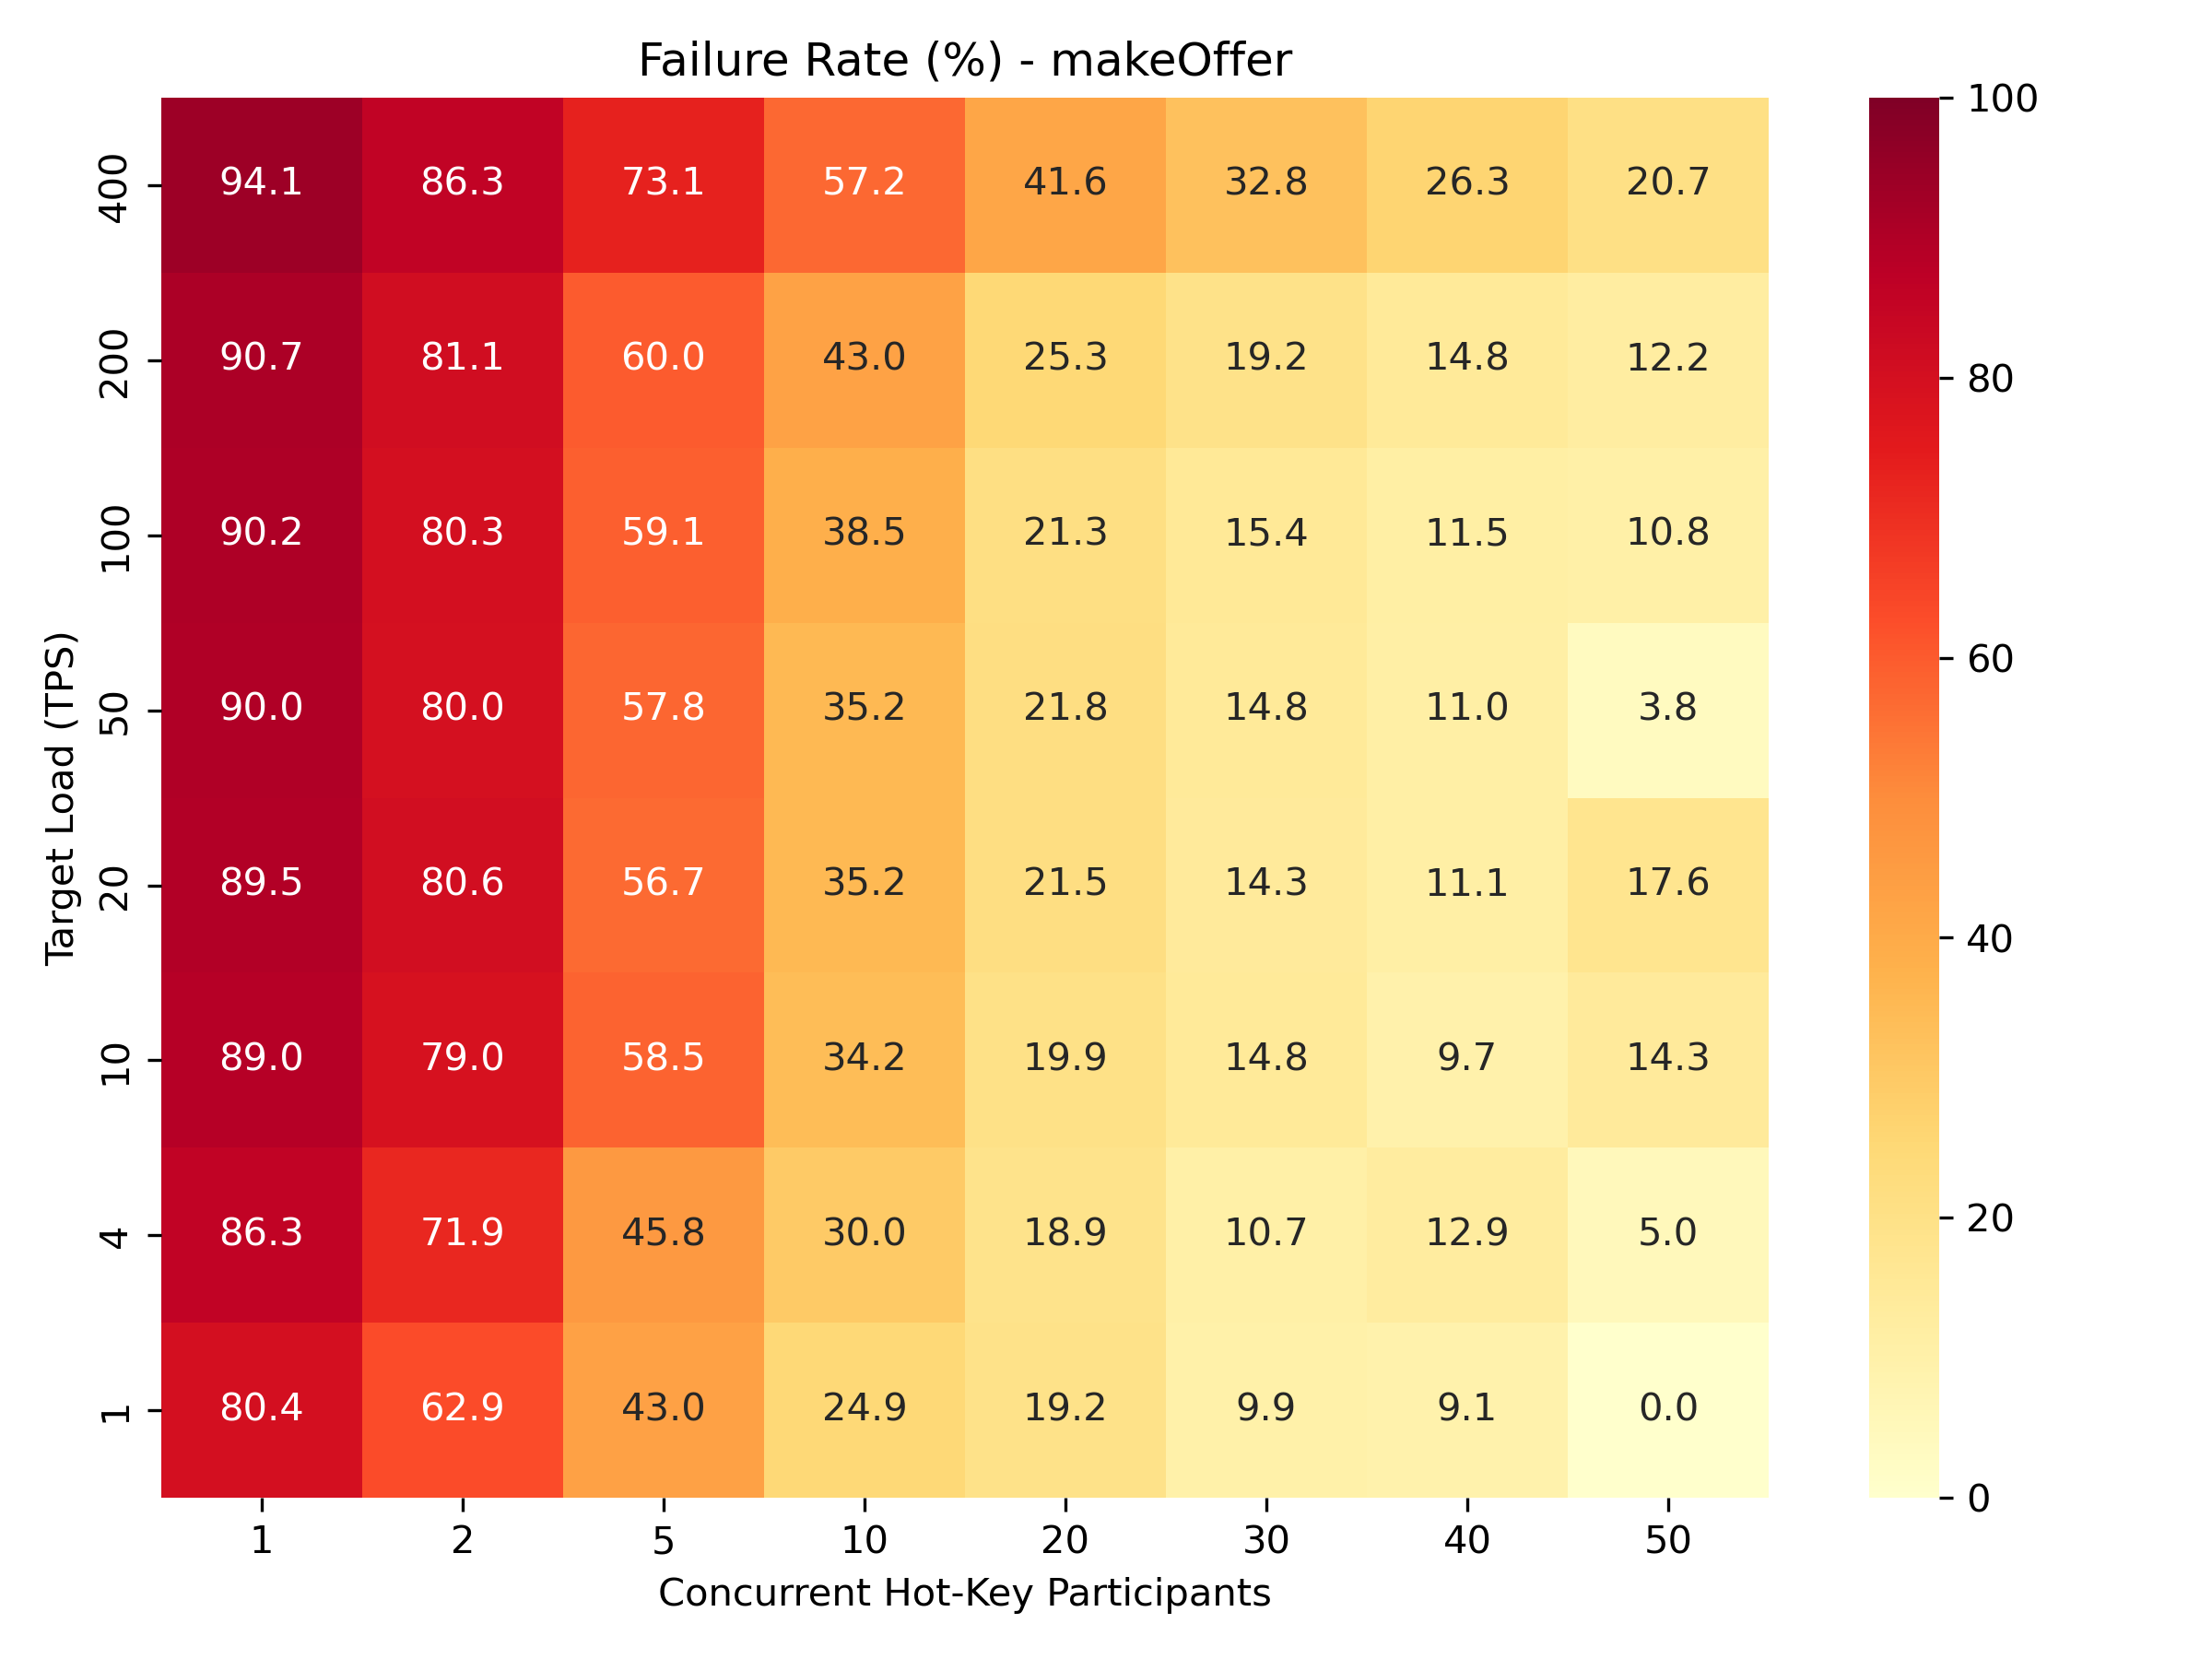
\includegraphics[width=\textwidth]{Figure_8a.png}
        \subcaption{makeOffer}
    \end{minipage}
    \hfill
    \begin{minipage}[b]{0.48\textwidth}
        \centering
        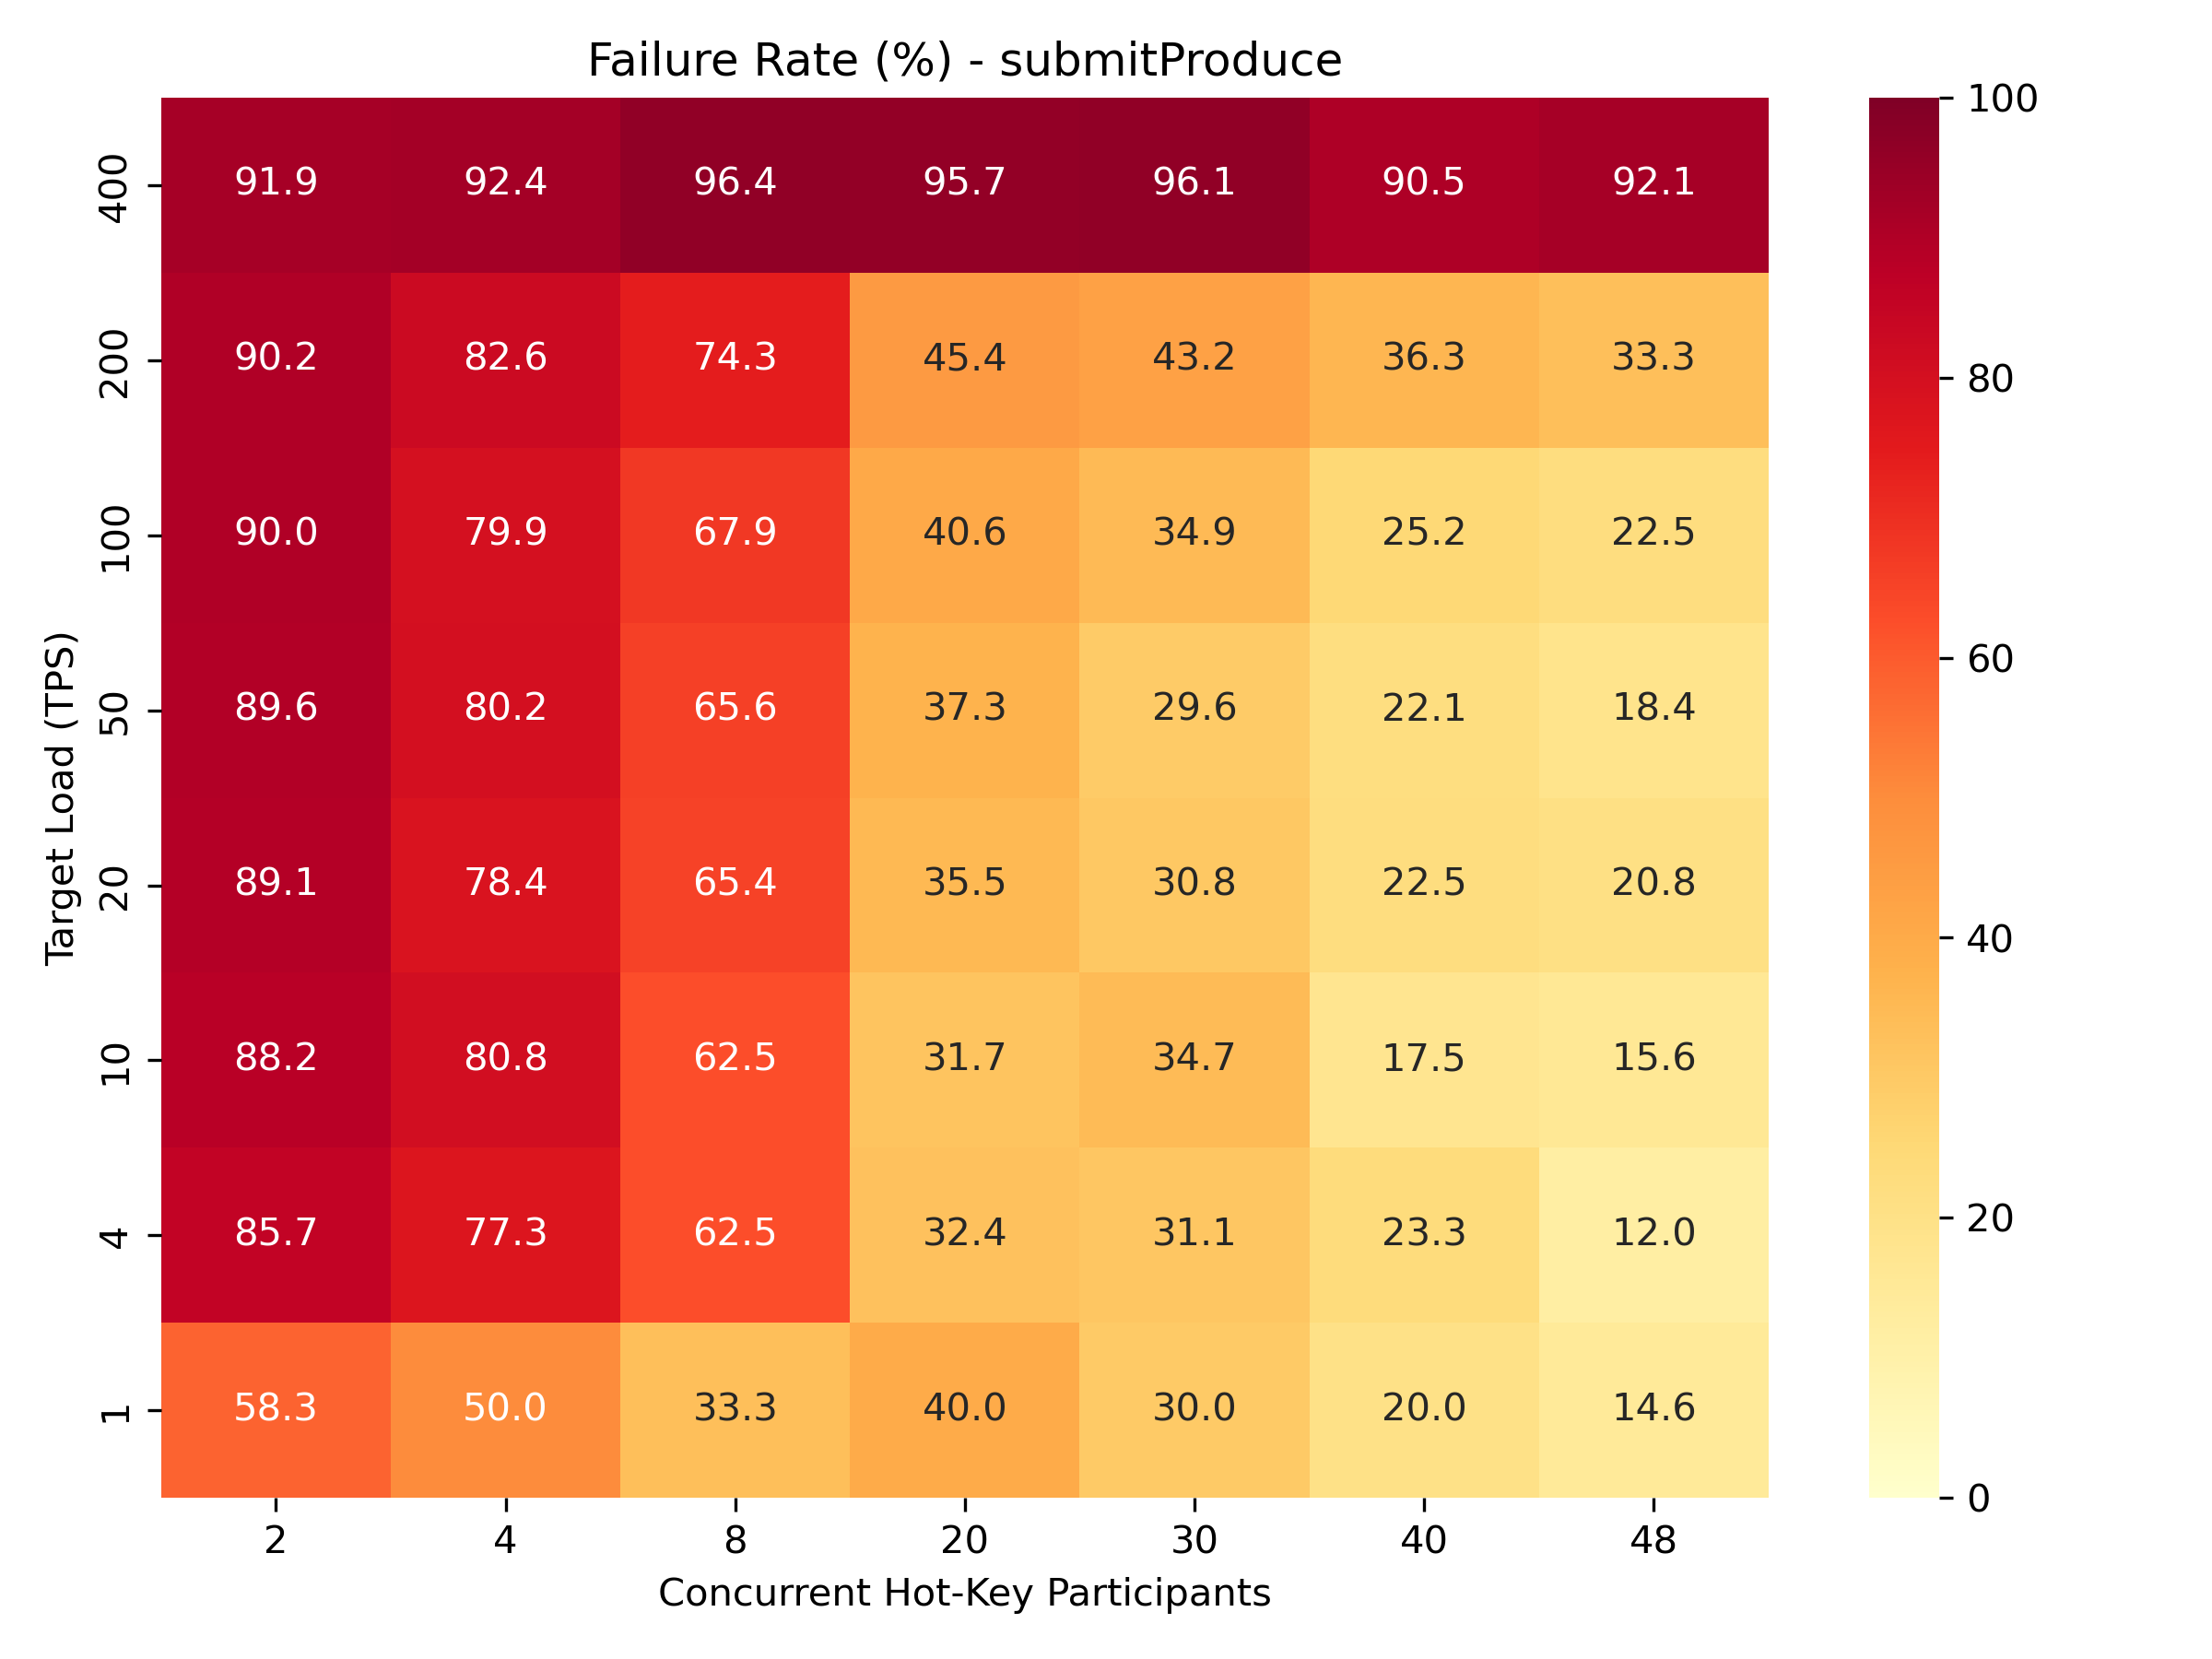
\includegraphics[width=\textwidth]{Figure_8b.png}
        \subcaption{submitProduce}
    \end{minipage}
    
    \vspace{0.3cm}
    
    \begin{minipage}[b]{0.48\textwidth}
        \centering
        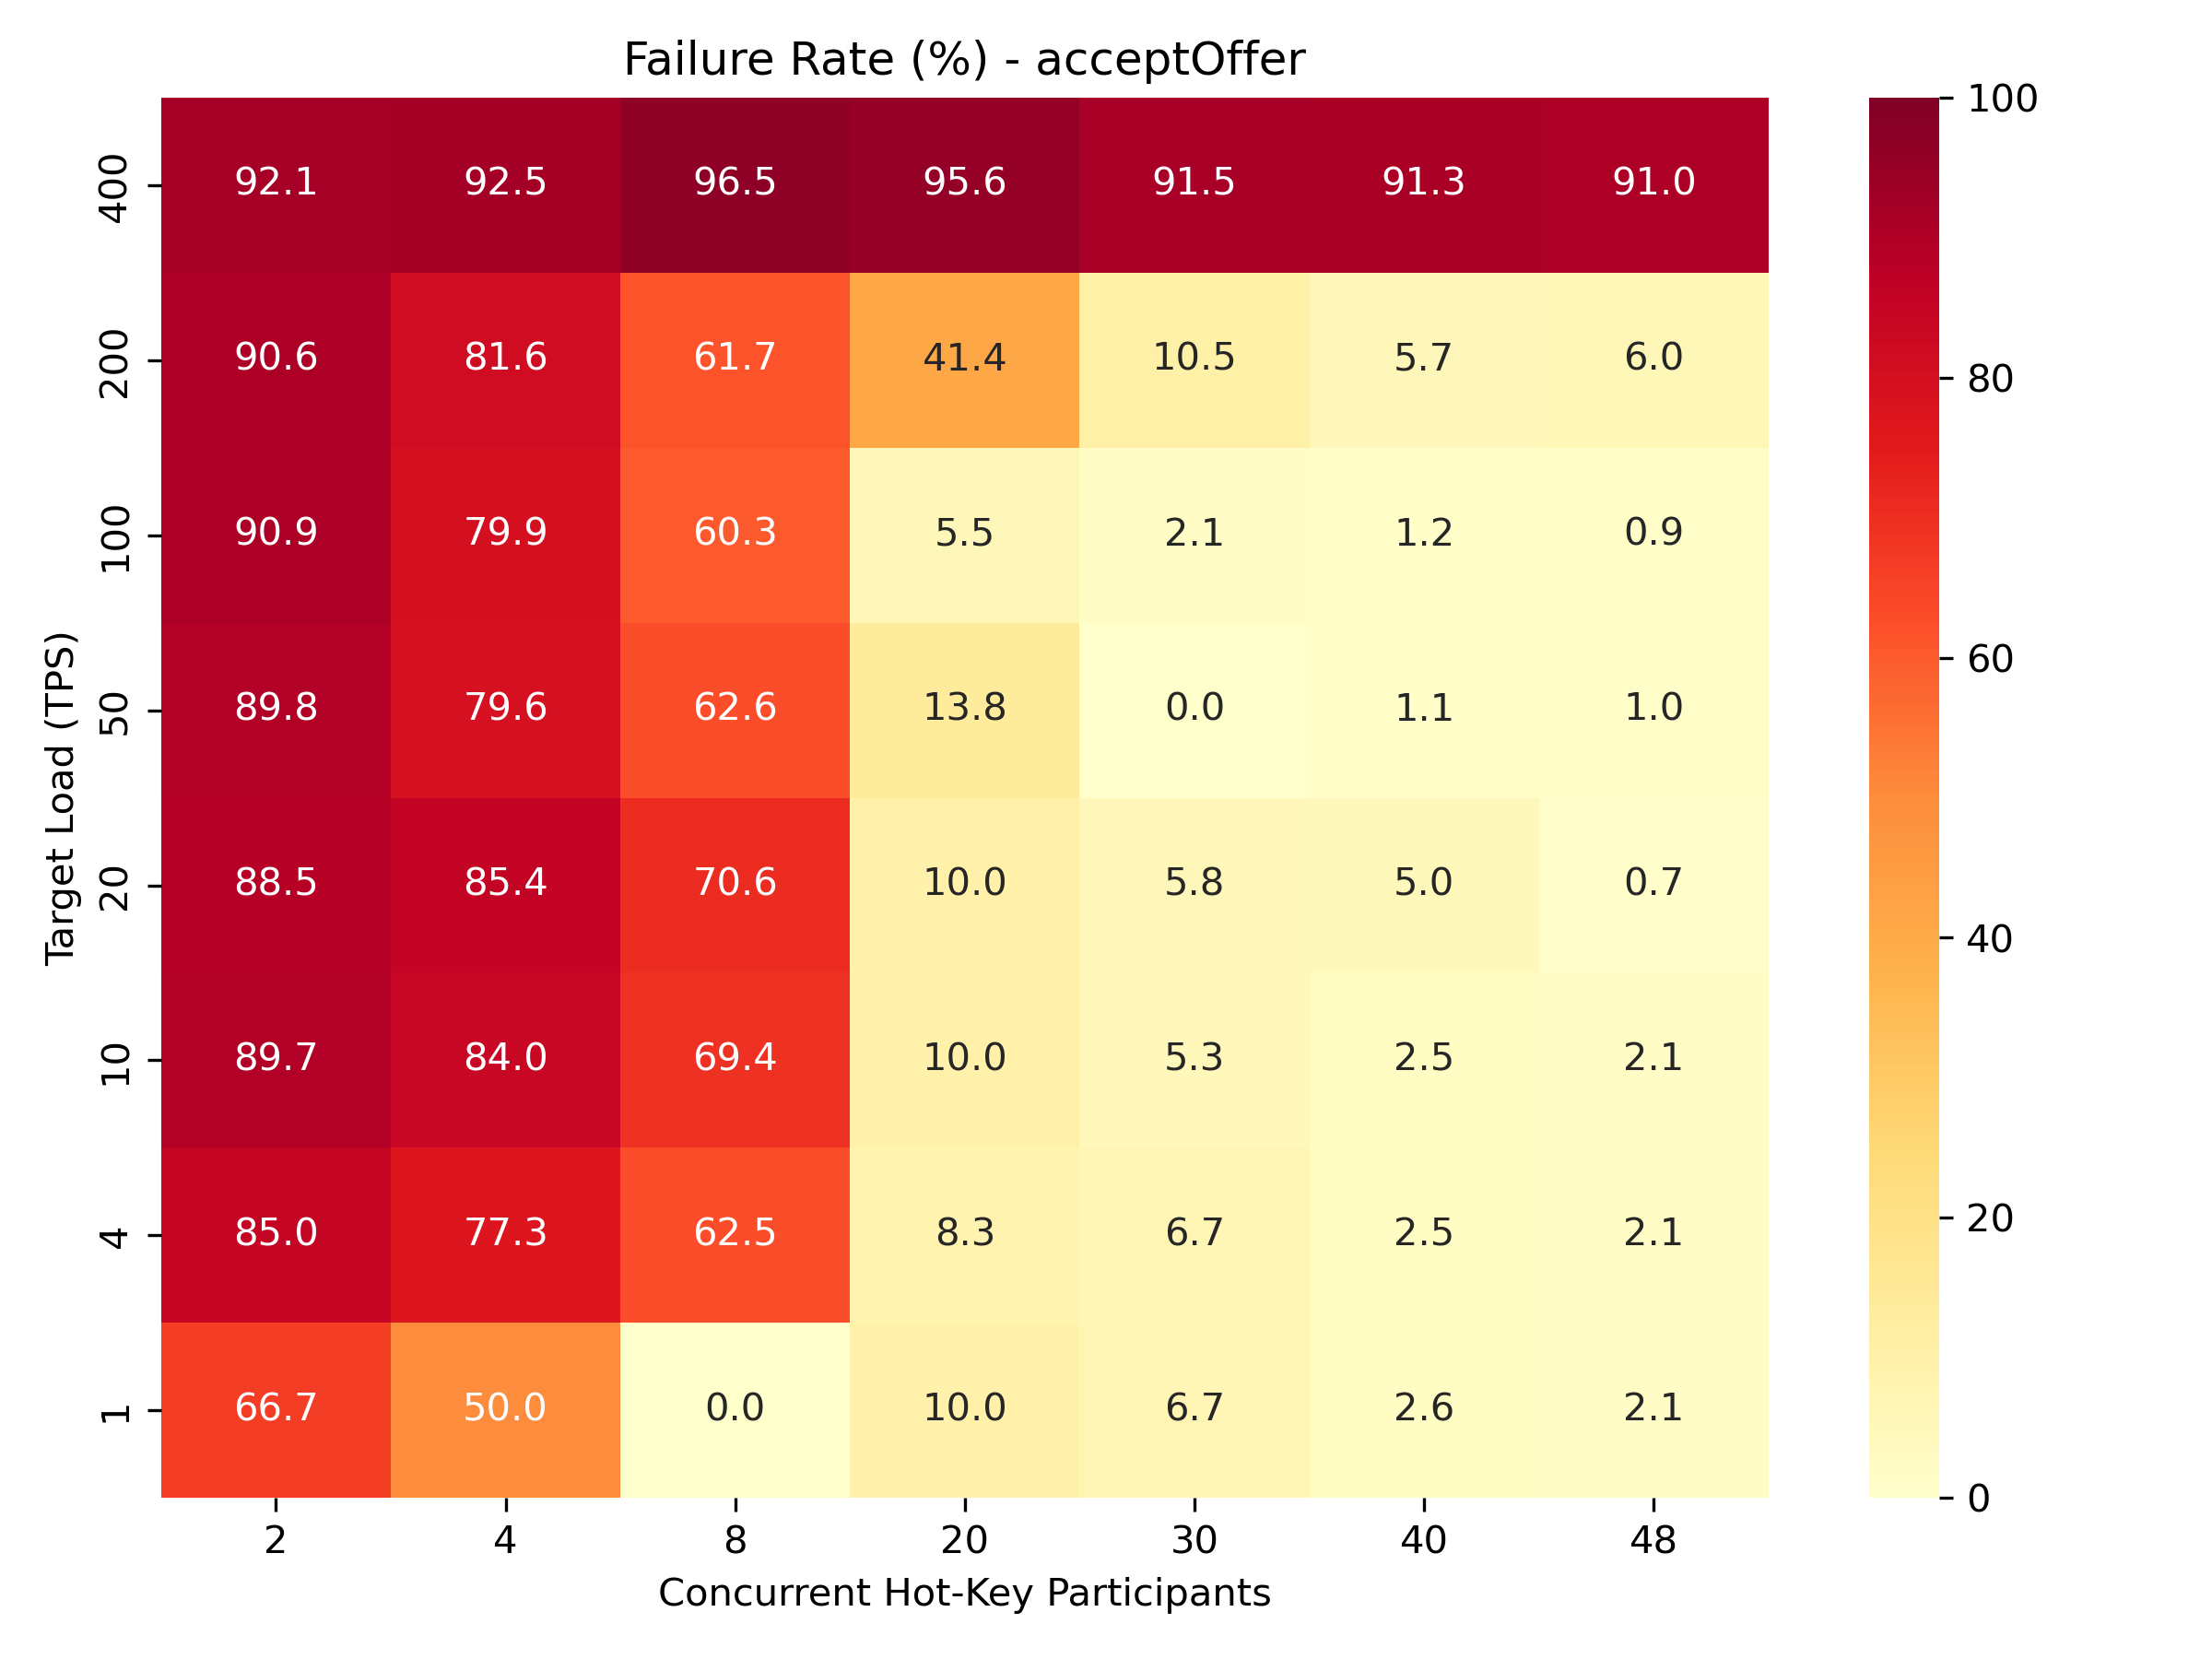
\includegraphics[width=\textwidth]{Figure_8c.png}
        \subcaption{acceptOffer}
    \end{minipage}
    \hfill
    \begin{minipage}[b]{0.48\textwidth}
        \centering
        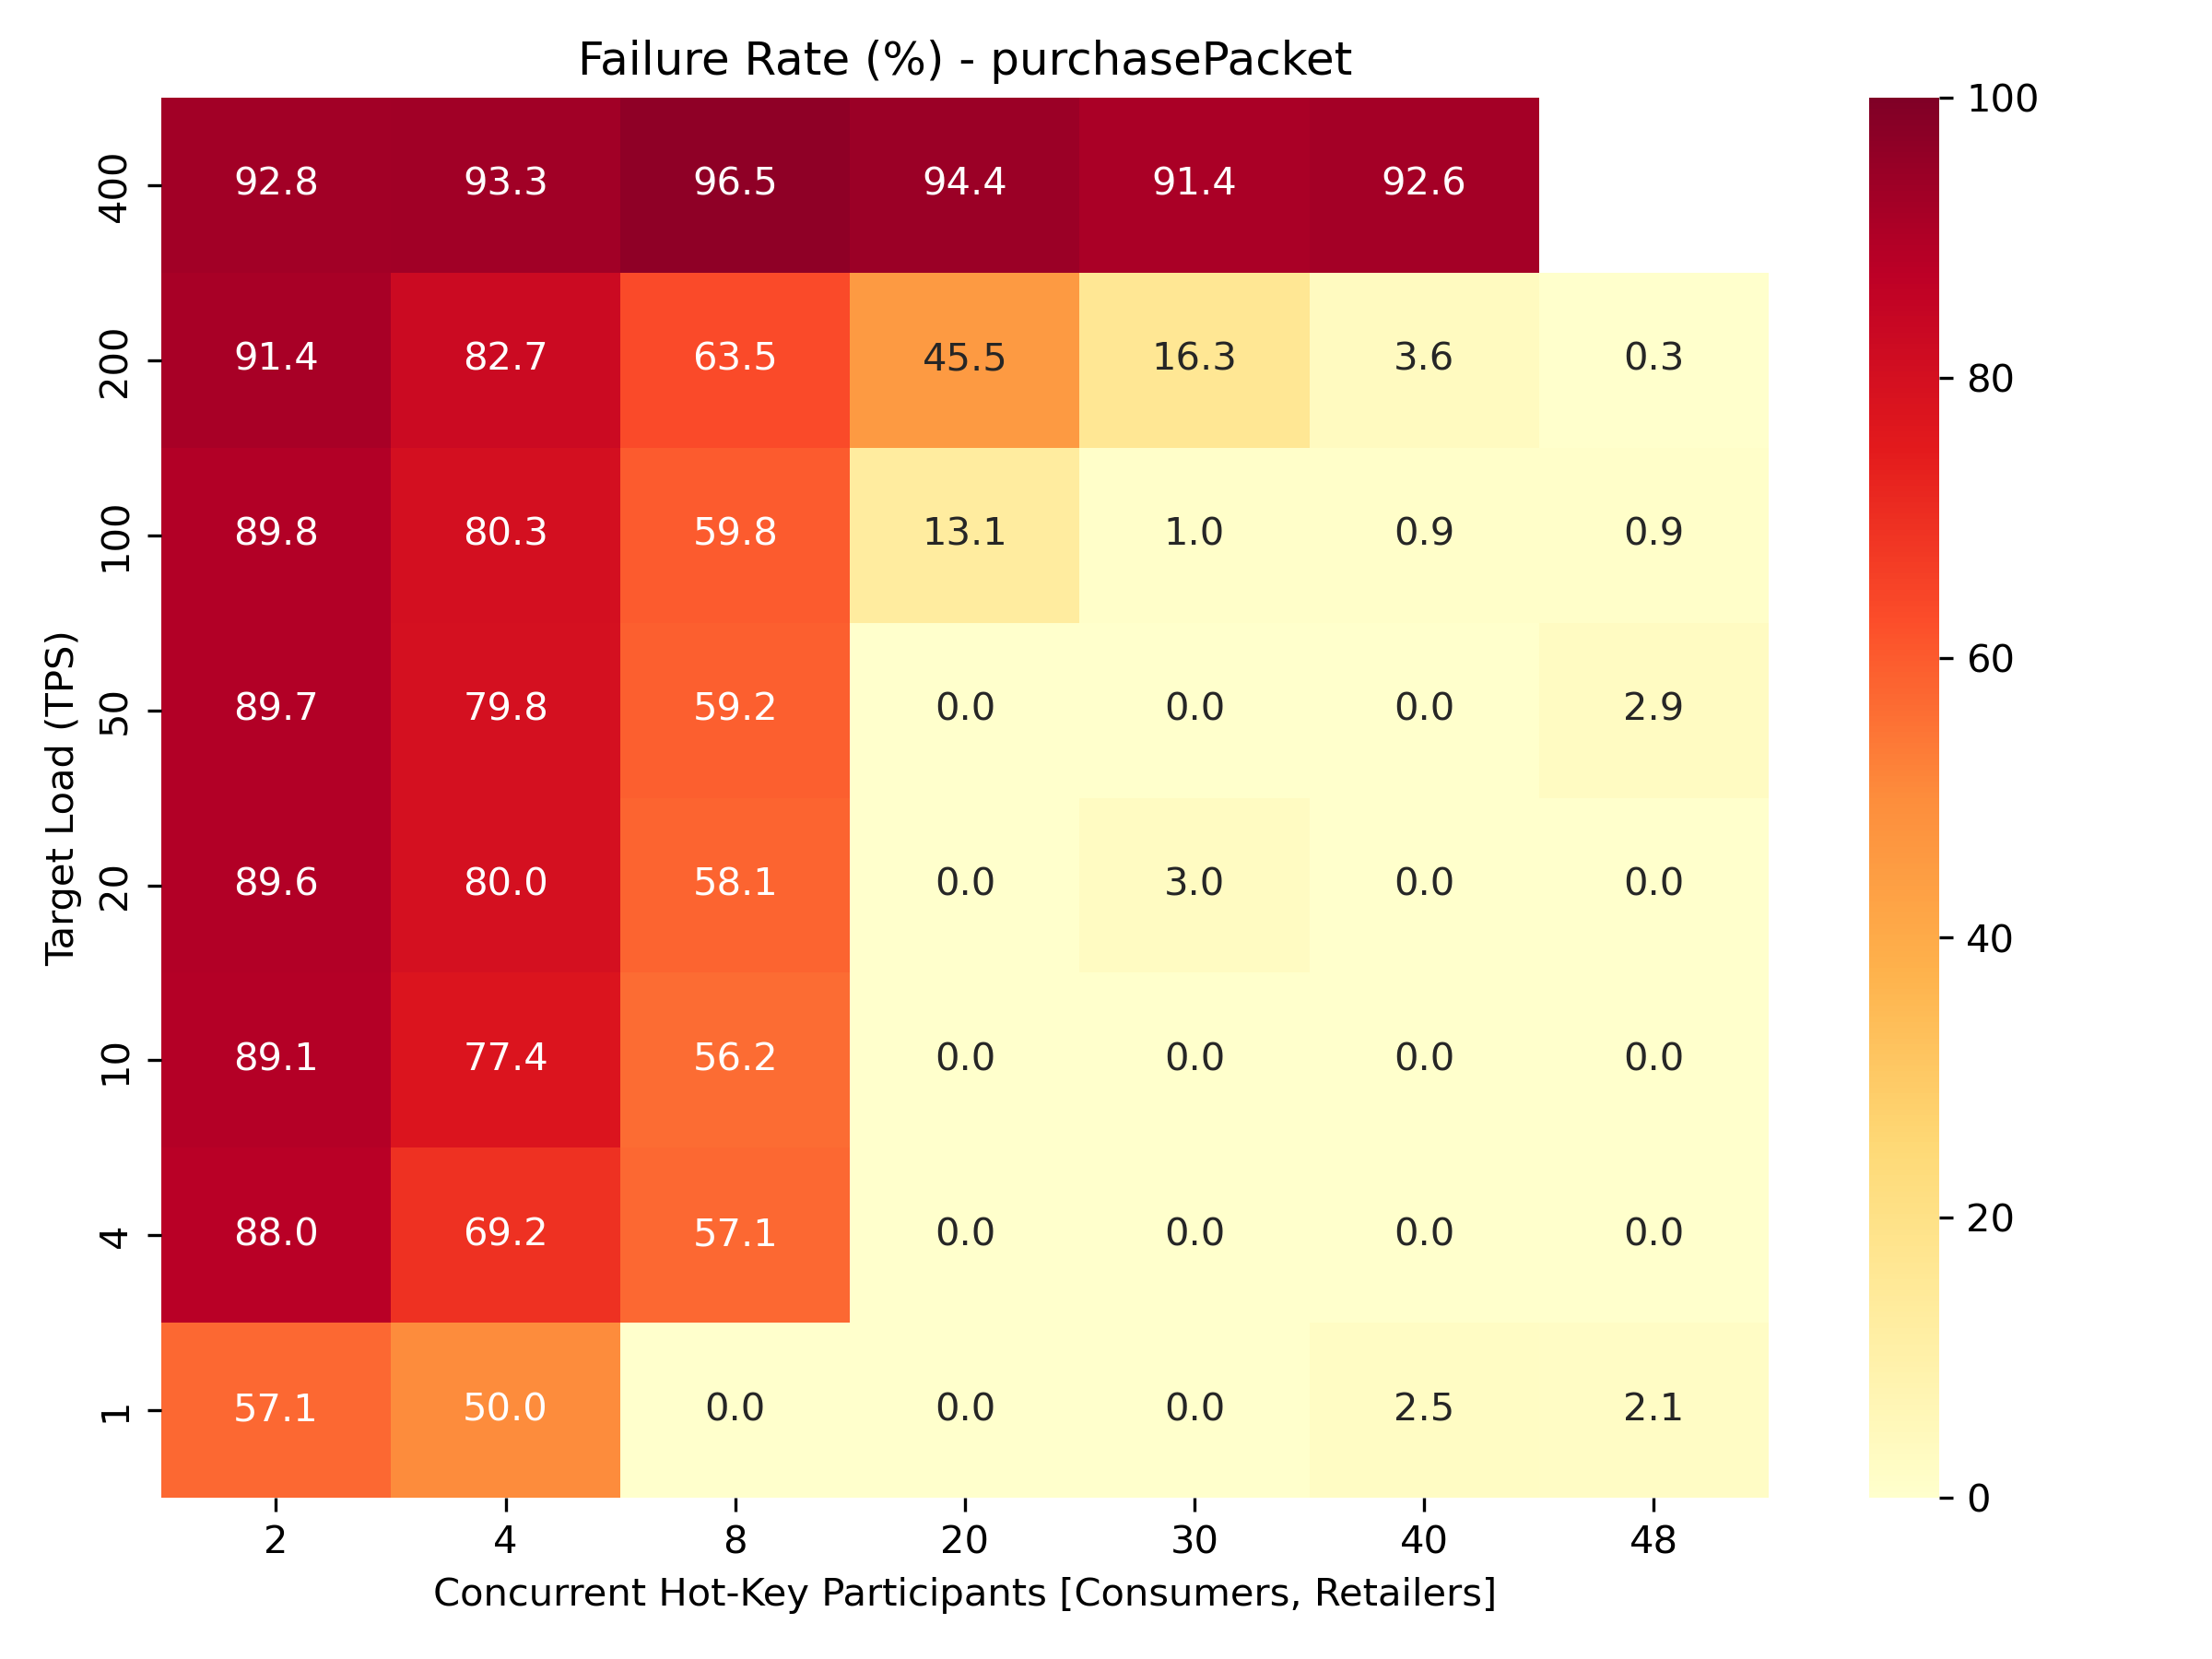
\includegraphics[width=\textwidth]{Figure_8d.png}
        \subcaption{purchasePacket}
    \end{minipage}
    \caption{Failure Rate Danger Zone matrices for the four core functions, mapping the non-linear boundaries of transaction timeouts across Target Load (TPS) and Concurrent Hot-Key Participants.}
    \label{fig:hotkey_failures}
\end{figure}

Figure \ref{fig:combined_50tps_failures} provides a cross-functional analysis of this compounding effect at a fixed load of 50 TPS. At this moderate send rate, the combination of restricted participant count and increasing network latency produced a sharp rise in failure rates across all evaluated functions. The two variables were found to be mutually reinforcing: a lower participant density intensified competition over shared ledger states, while greater latency extended the period of vulnerability to concurrent write conflicts. The combined effect consistently exceeded the impact of either variable in isolation.

\begin{figure}[H]
    \centering
    \begin{minipage}[b]{0.48\textwidth}
        \centering
        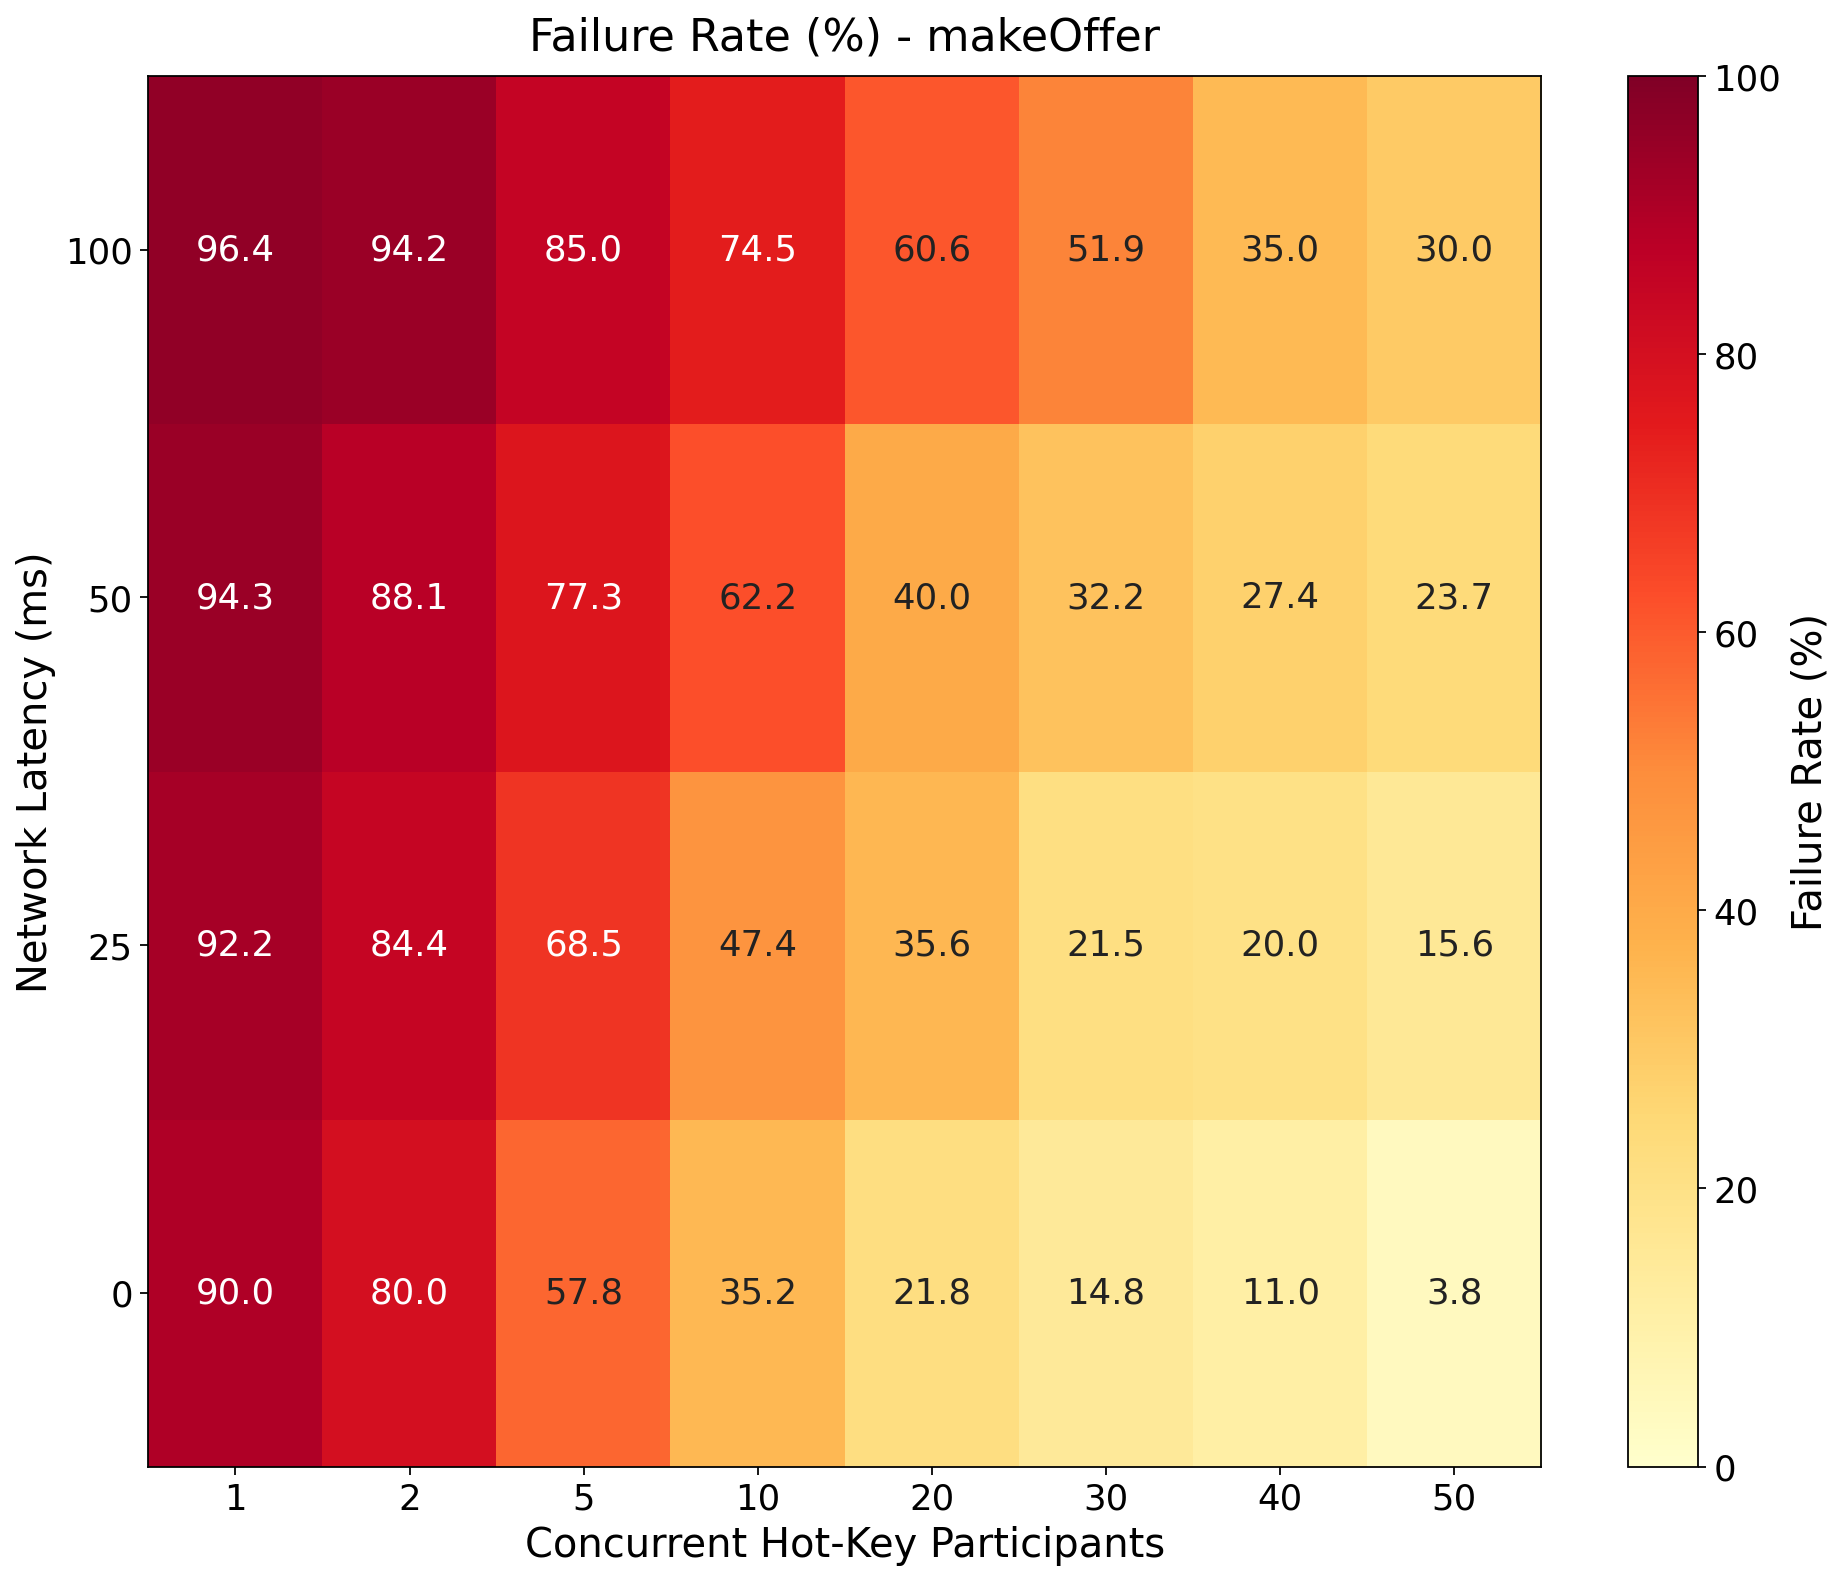
\includegraphics[width=\textwidth]{Figure_9a.png}
        \subcaption{makeOffer}
    \end{minipage}
    \hfill
    \begin{minipage}[b]{0.48\textwidth}
        \centering
        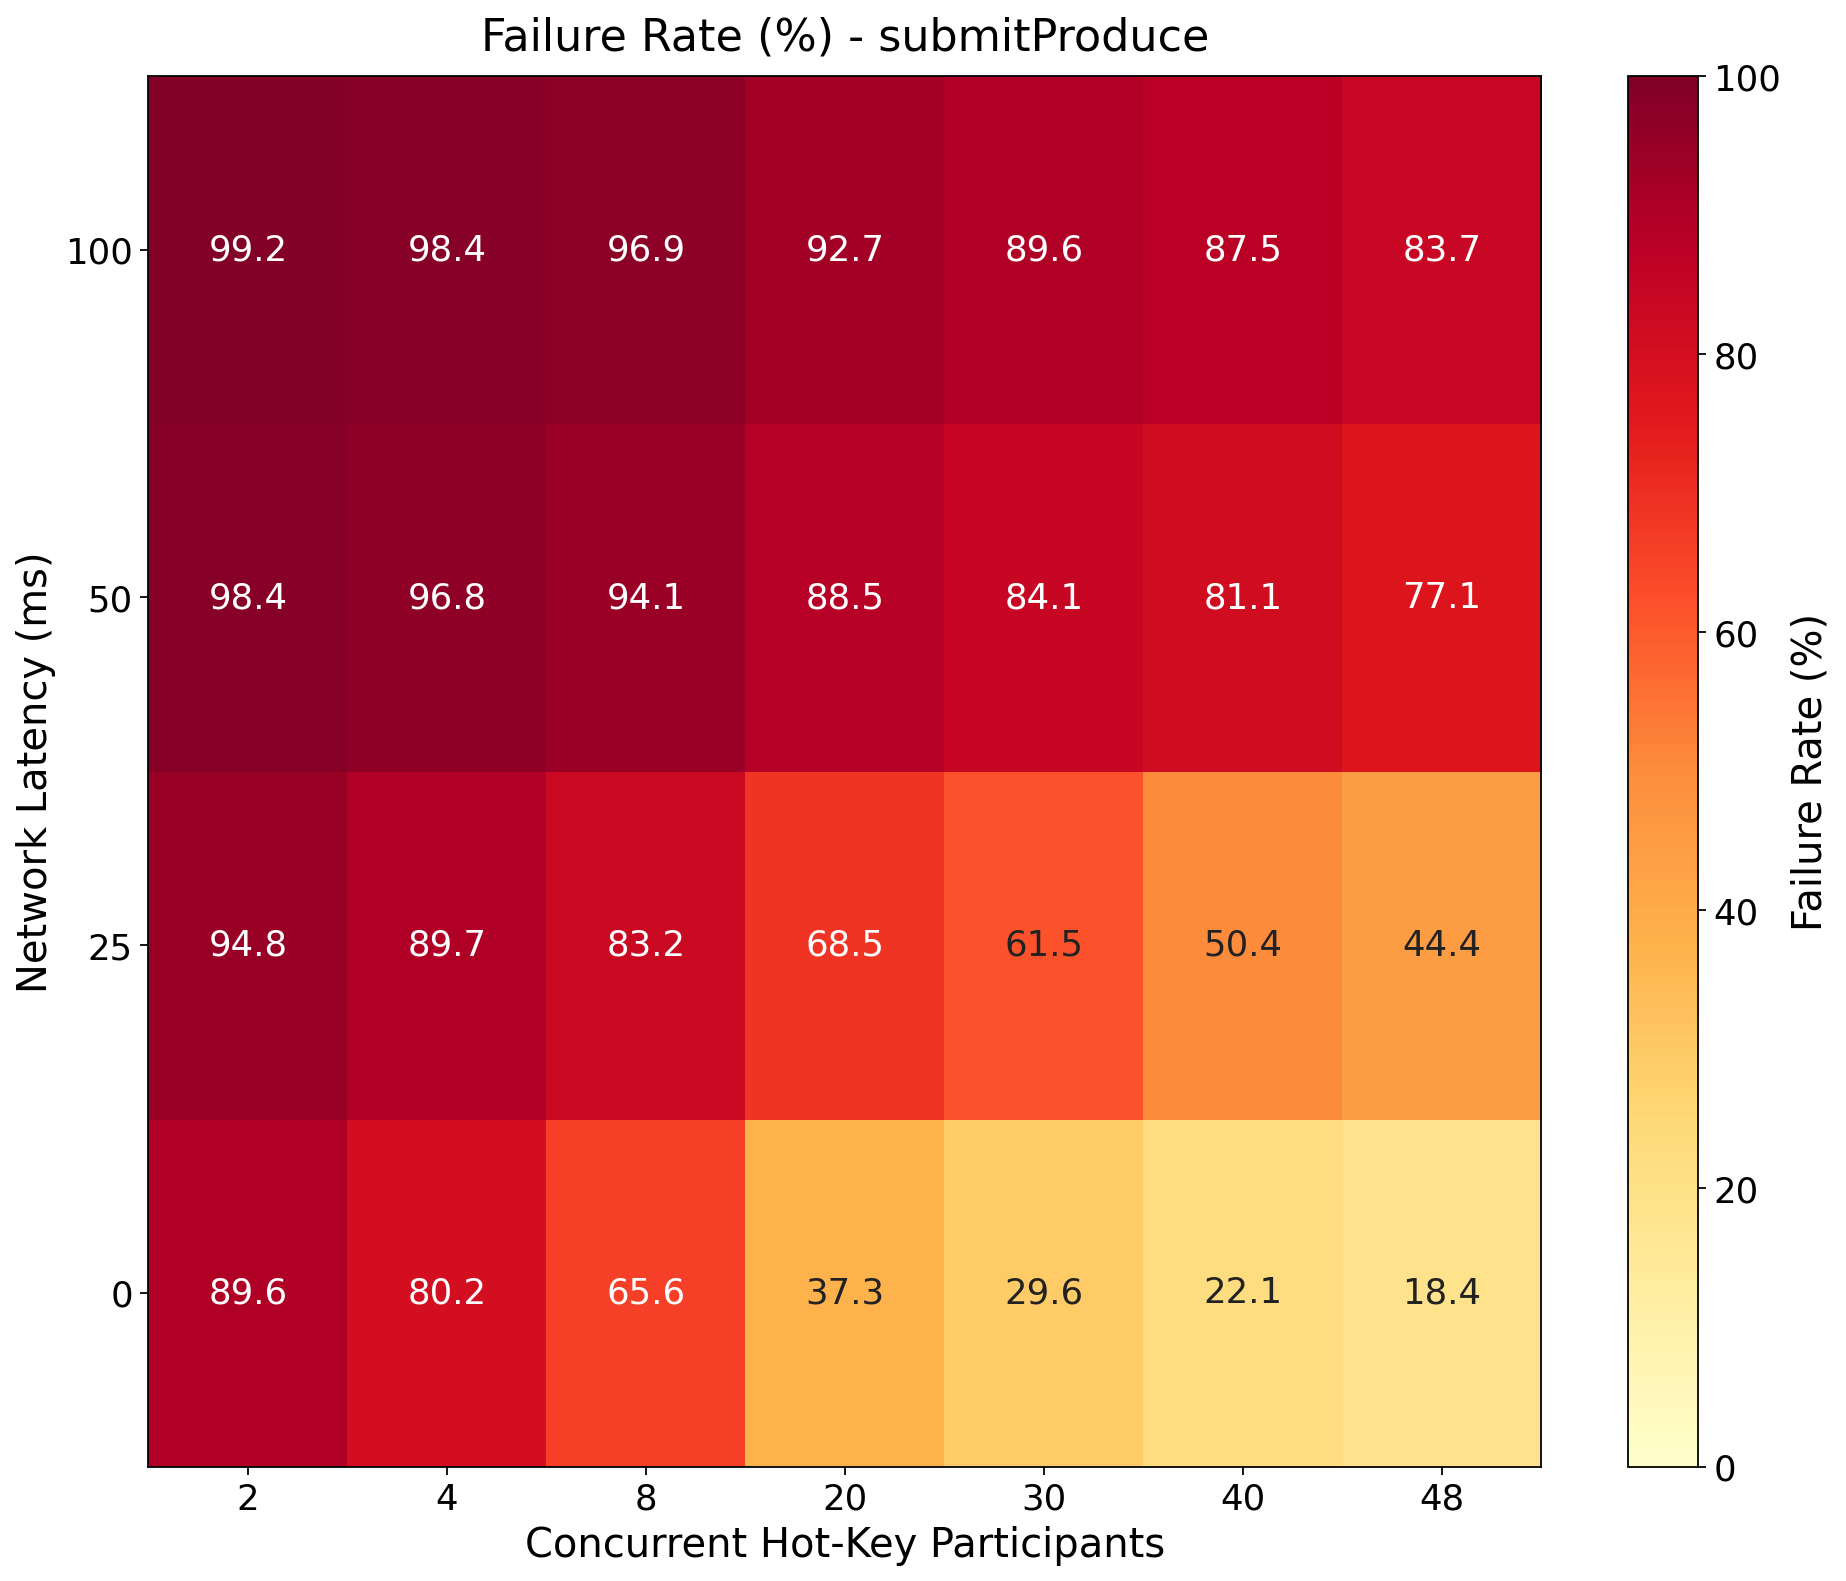
\includegraphics[width=\textwidth]{Figure_9b.png}
        \subcaption{submitProduce}
    \end{minipage}

    \vspace{0.3cm}

    \begin{minipage}[b]{0.48\textwidth}
        \centering
        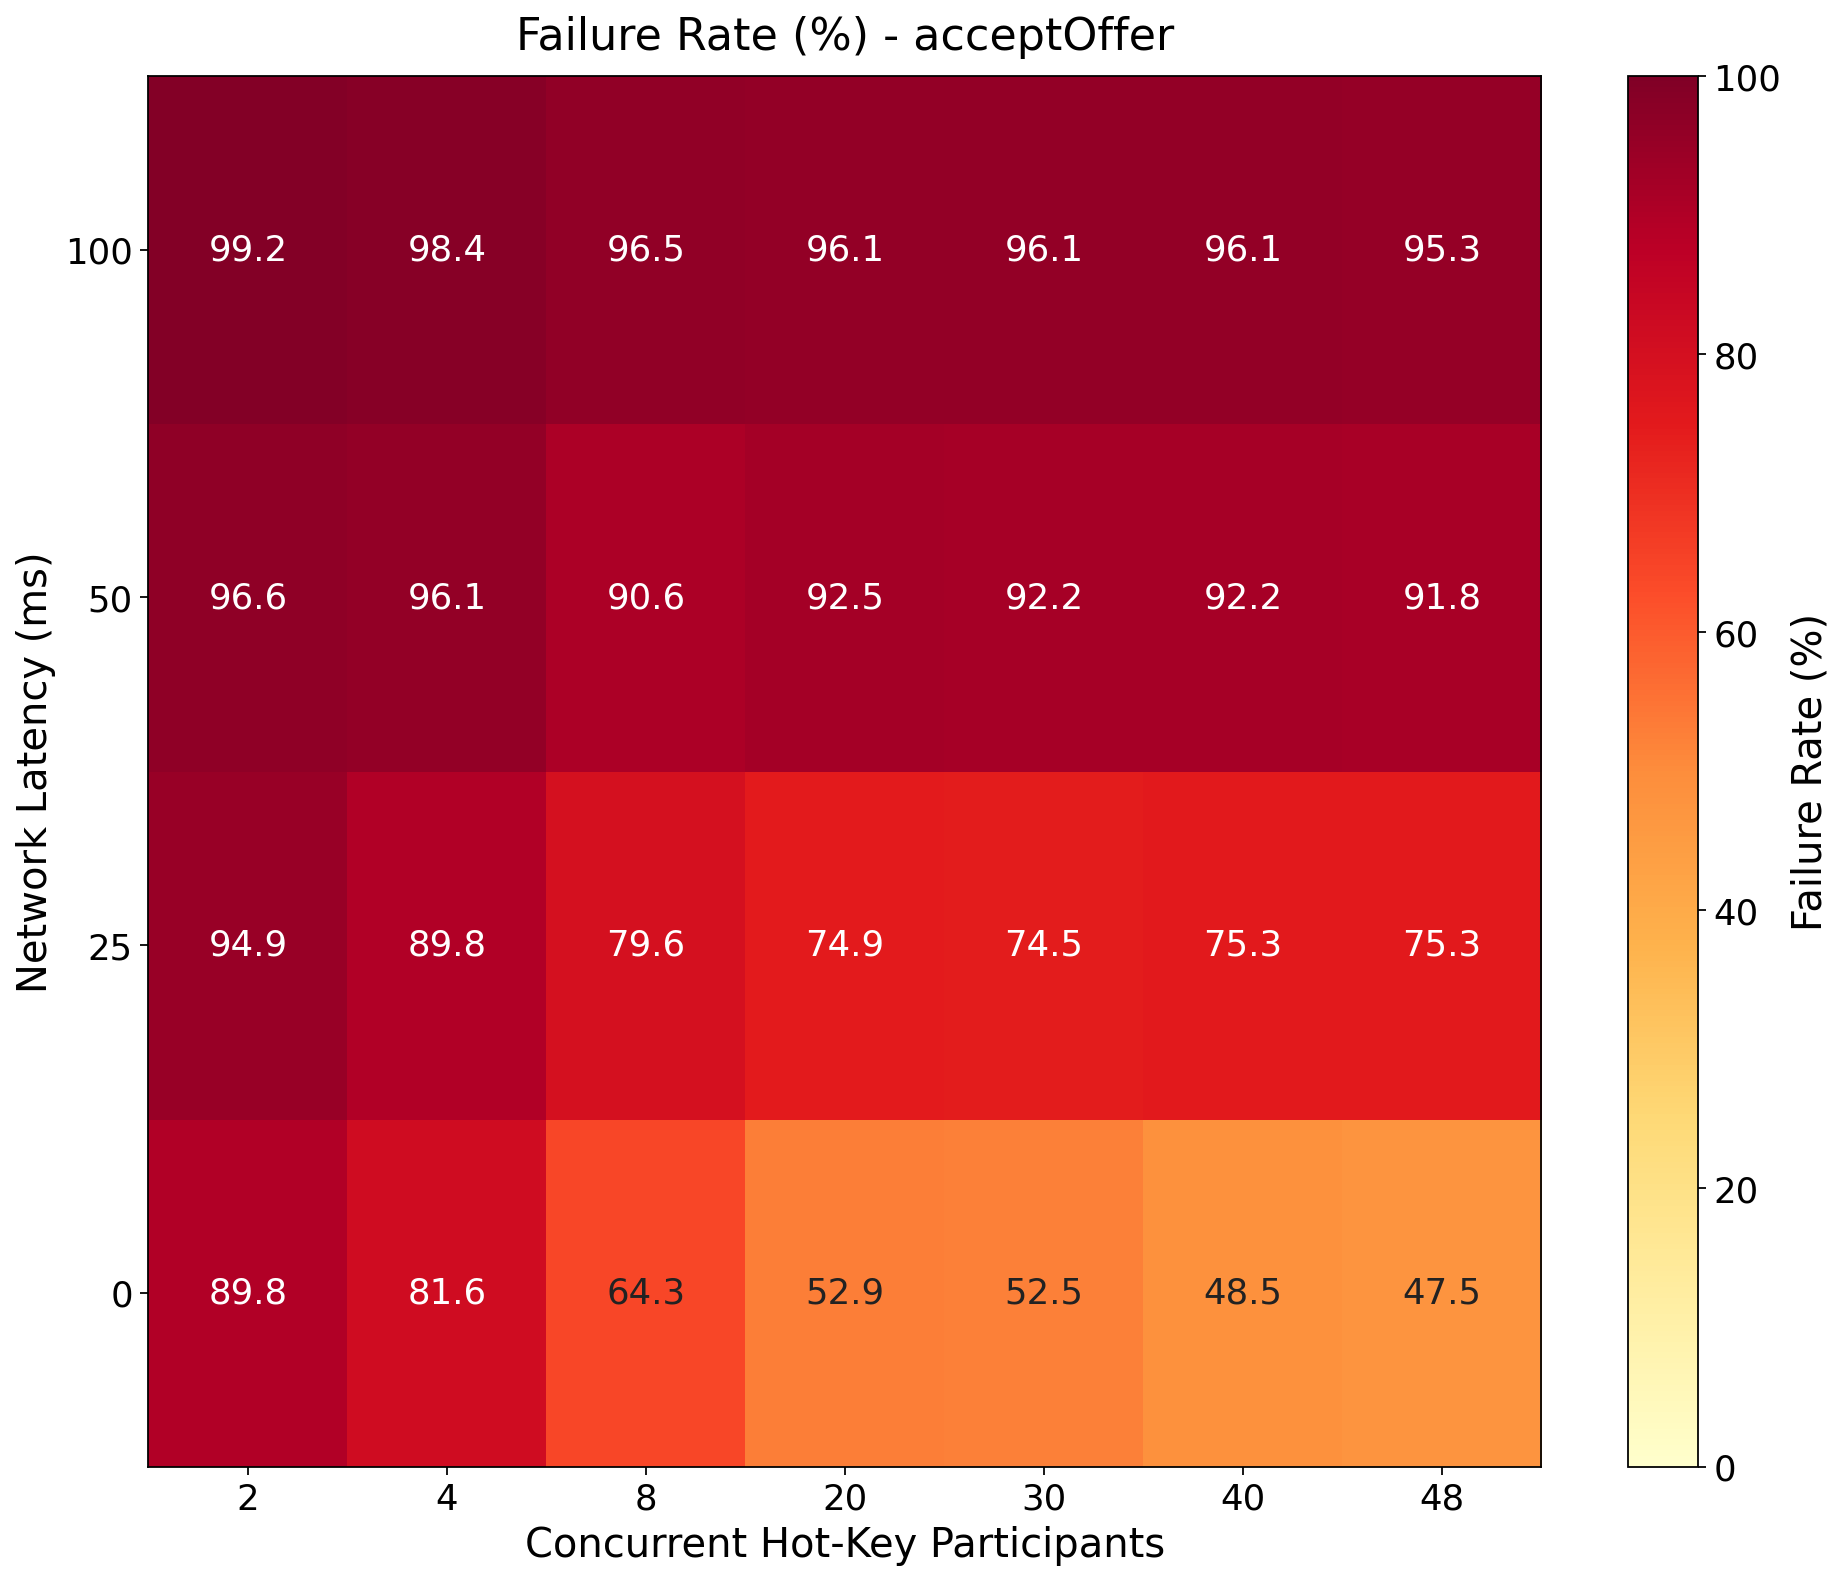
\includegraphics[width=\textwidth]{Figure_9c.png}
        \subcaption{acceptOffer}
    \end{minipage}
    \hfill
    \begin{minipage}[b]{0.48\textwidth}
        \centering
        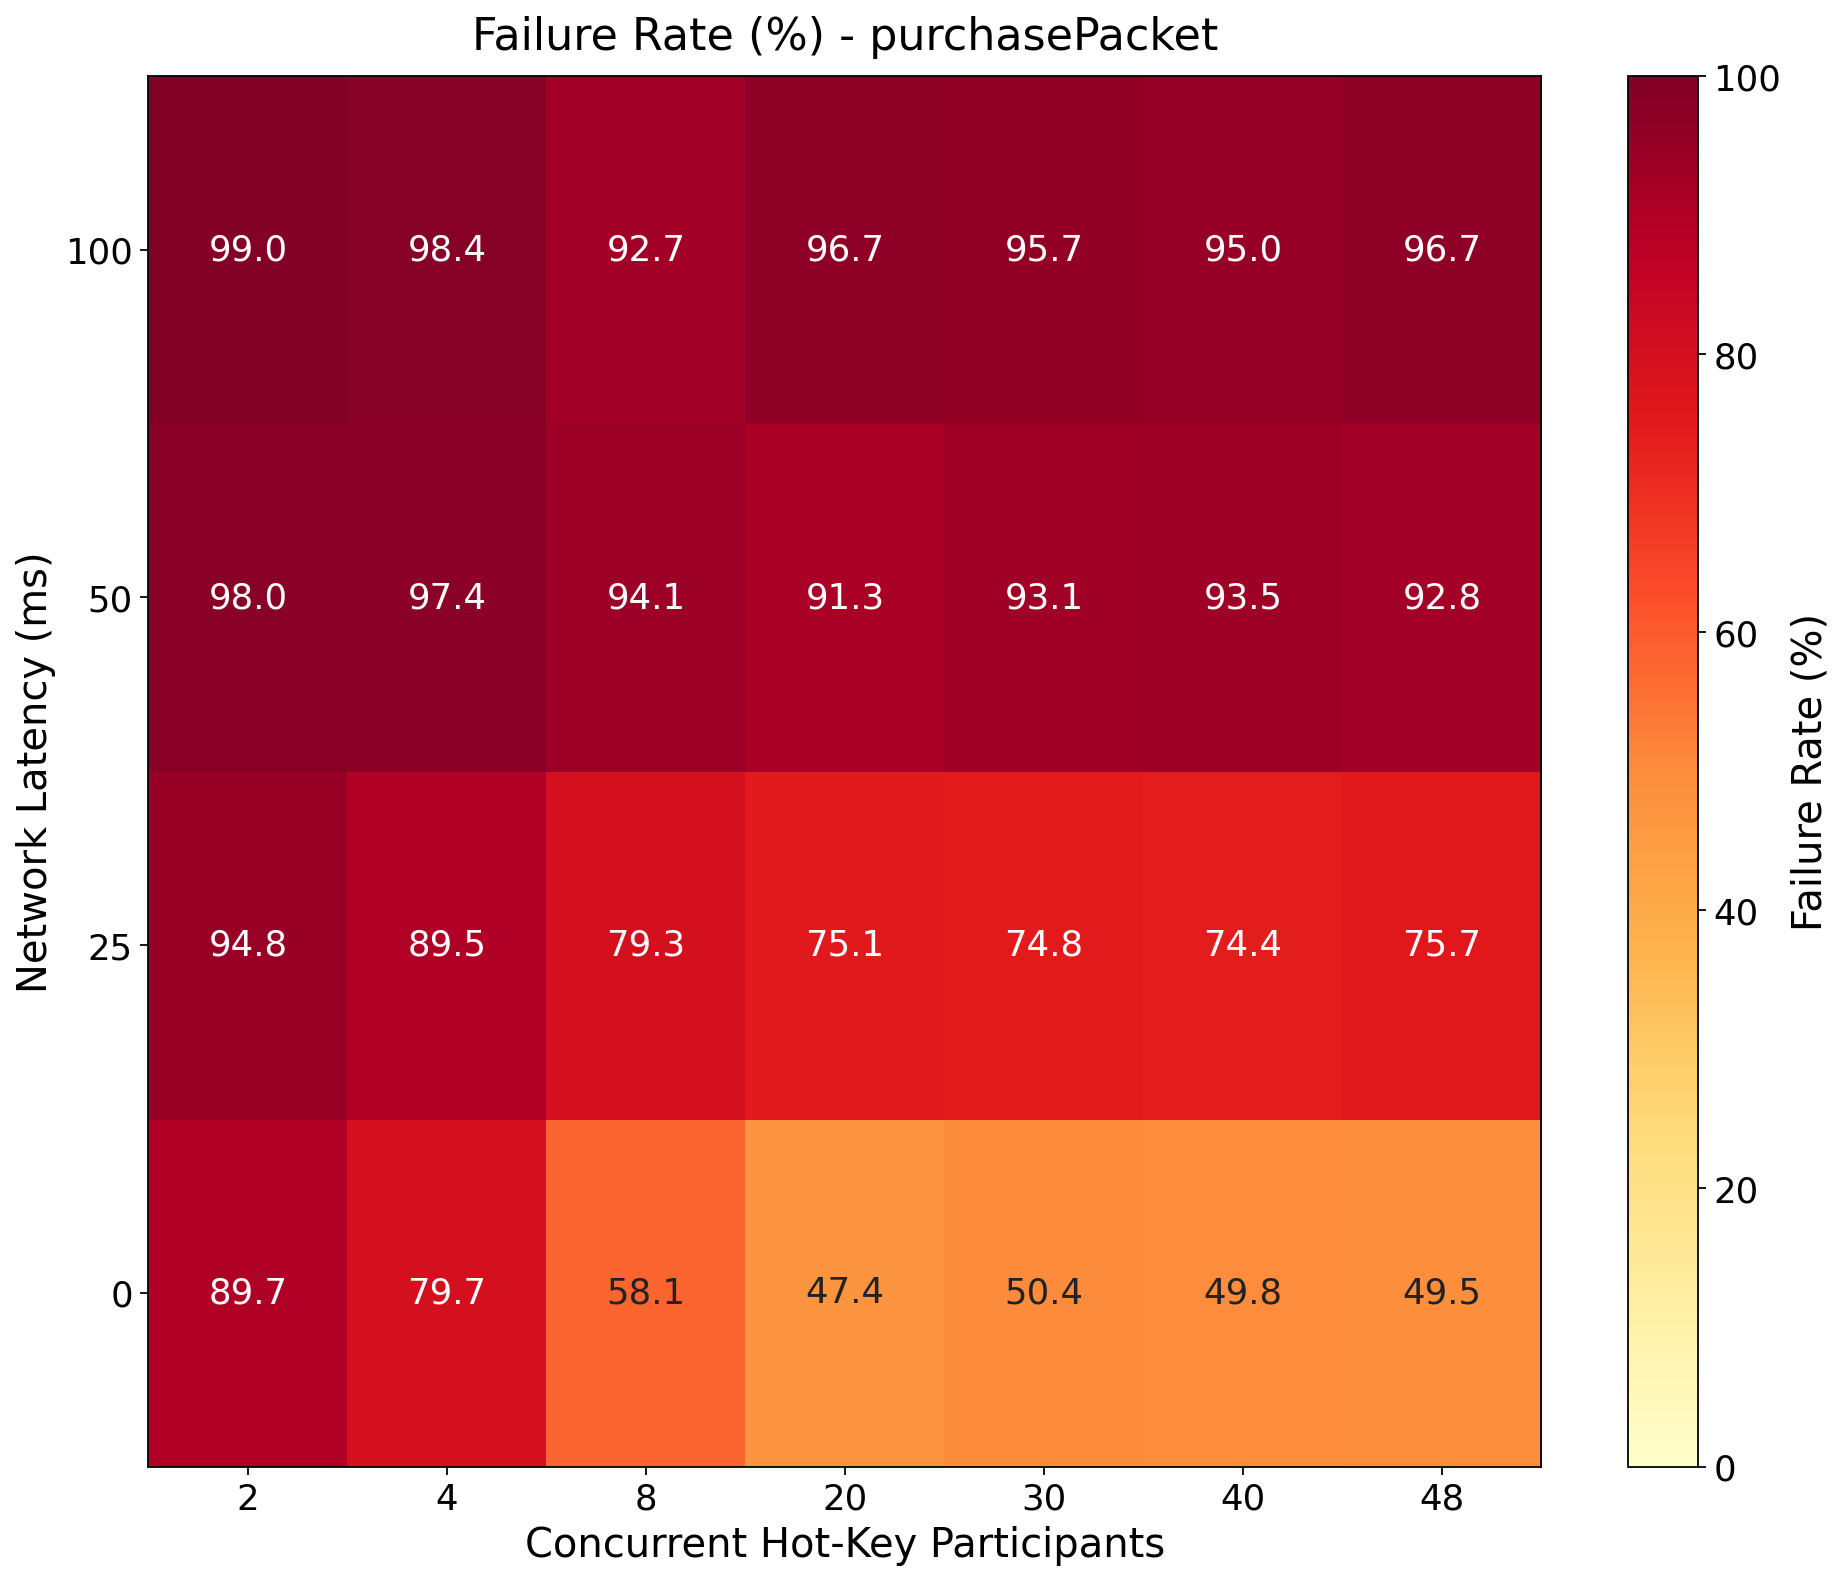
\includegraphics[width=\textwidth]{Figure_9d.png}
        \subcaption{purchasePacket}
    \end{minipage}
    \caption{Failure rate matrices for the four core functions at exactly 50 TPS, mapping the interaction between network latency, concurrent hot-key participants, and transaction failure rate.}
    \label{fig:combined_50tps_failures}
\end{figure}







\subsection{Predictive Benchmarking}

While the empirical benchmarking characterised the performance boundaries of the supply chain chaincode, it did not fully account for the compound interactions between contributing variables. Transaction failures are governed by the joint influence of transaction load, participant density, per-transaction write complexity, and network latency. To model these interactions and identify their relative contributions, a supervised machine learning framework was applied to the Caliper benchmark dataset. The training corpus spanned participant counts from 1 to 24 and send rates from 1 to 500 TPS across all primary chaincode functions. To verify the presence of multi-collinearity and the linear relationships between these extracted features and the resulting throughput and failure metrics, a feature correlation matrix was initially computed (Figure \ref{fig:correlation_heatmap}).

\begin{figure}[H]
    \centering
    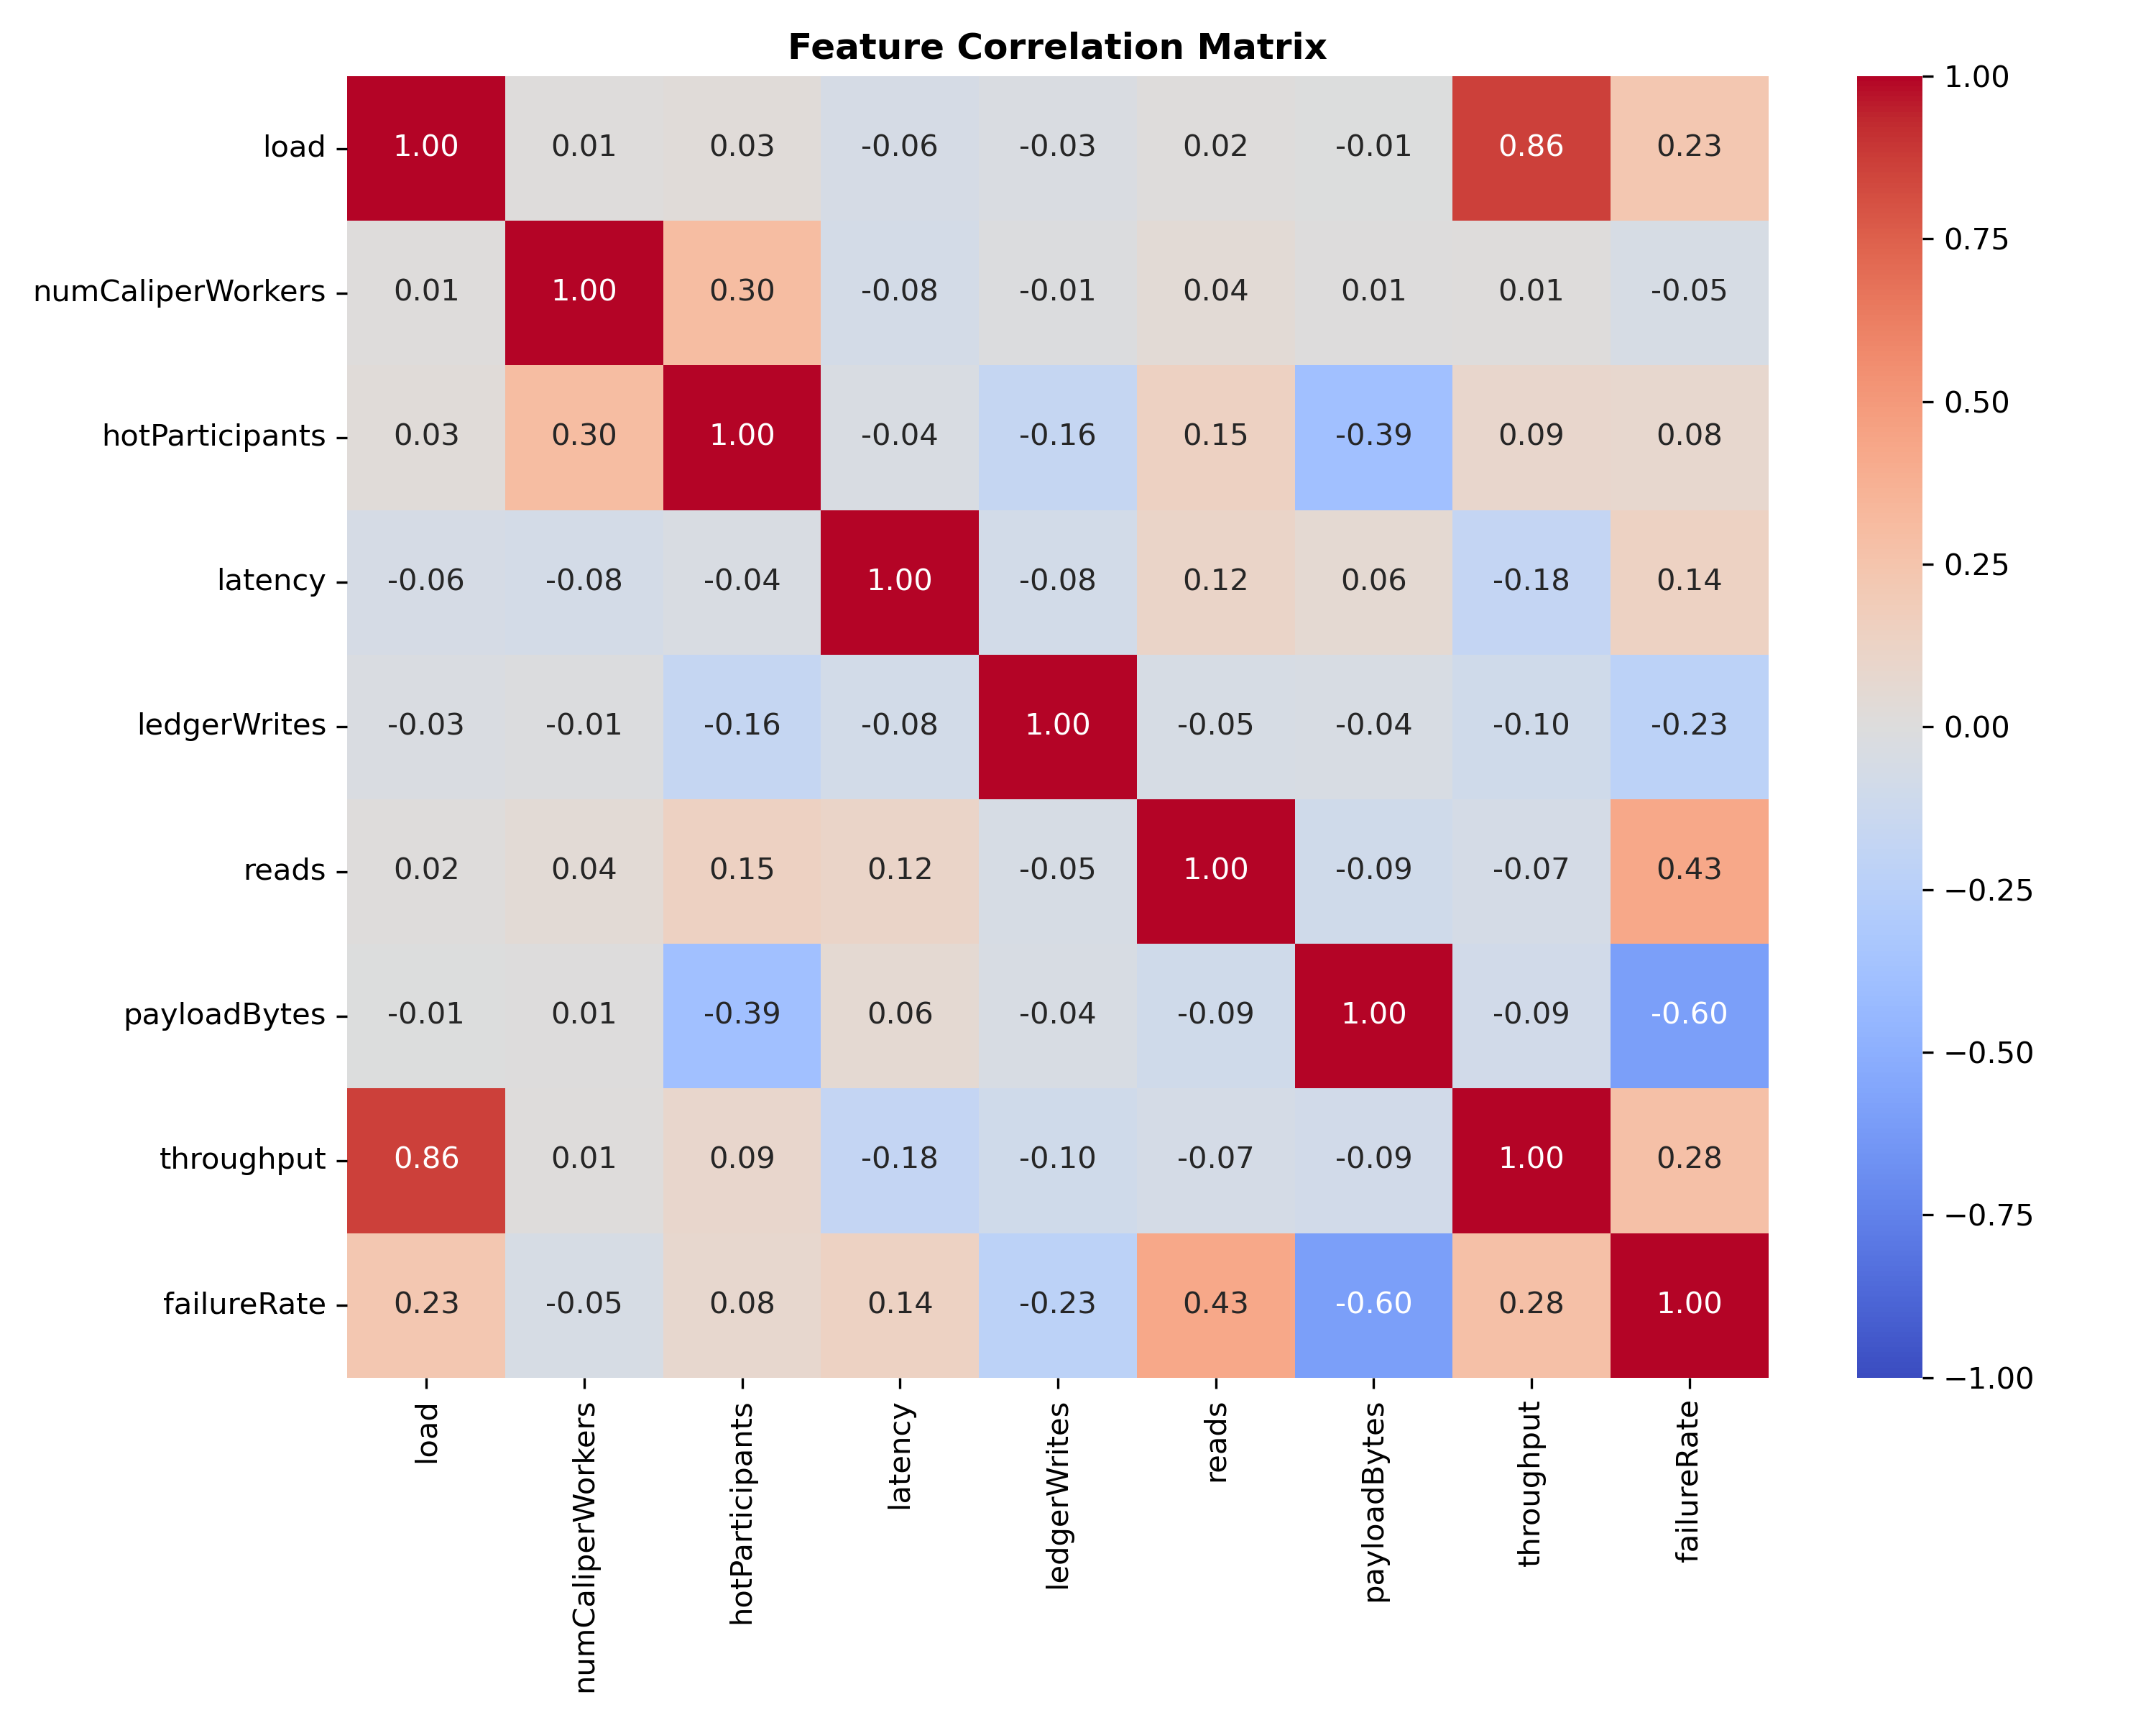
\includegraphics[width=0.8\textwidth]{Figure_10.png}
\caption{Feature Correlation Matrix showing the relationships between network variables, throughput, and failure rate.}
    \label{fig:correlation_heatmap}
\end{figure}


\subsubsection{Model Selection}
Consistent with the theoretical limitations outlined in the methodology, Linear Regression struggled to accurately model the non-linear, threshold-driven nature of MVCC transaction failures. The tree-based ensembles performed significantly better. The Random Forest regressor was selected as the primary analytical model for the remainder of this study due to its strong generalisation performance across both prediction targets and its capacity to distribute feature importance across multiple variables without disproportionate reliance on any single predictor.

\subsubsection{Throughput Prediction}
Table \ref{tab:throughput_performance} presents the comparative predictive performance of each model for transaction throughput.

\begin{table}[ht]
\centering
\caption{Comparative Predictive Performance (Target: Transaction Throughput)}
\label{tab:throughput_performance}
\resizebox{0.8\columnwidth}{!}{%
\begin{tabular}{|l|c|c|c|}
\hline
\textbf{Machine Learning Model} & \textbf{$R^2$ Score} & \textbf{MAE} & \textbf{RMSE} \\
\hline
Linear Regression & 0.8148 & 23.355 & 39.159 \\
Gradient Boosting & 0.9143 & 8.340 & 20.541 \\
\textbf{Random Forest Regressor} & \textbf{0.9236} & \textbf{11.933} & \textbf{25.145} \\
\hline
\end{tabular}%
}
\end{table}

The Random Forest model demonstrated strong generalisation for throughput prediction across the full experimental range, while also providing stable feature-importance estimates across both prediction targets. As shown in Figure \ref{fig:throughput-feature-importance}, transaction send rate (\textbf{Load}) emerged as the dominant predictor, contributing 81.1\% of the total feature importance. Secondary structural variables---\textbf{Ledger Writes} (5.7\%), \textbf{Network Latency} (5.2\%), and \textbf{Payload Bytes} (3.2\%)---each contributed meaningfully to the model's predictive capacity. These findings confirm that, while raw send rate is the primary throughput determinant, chaincode write complexity and network conditions impose measurable structural limits on attainable throughput.

\begin{figure}[H]
\centering
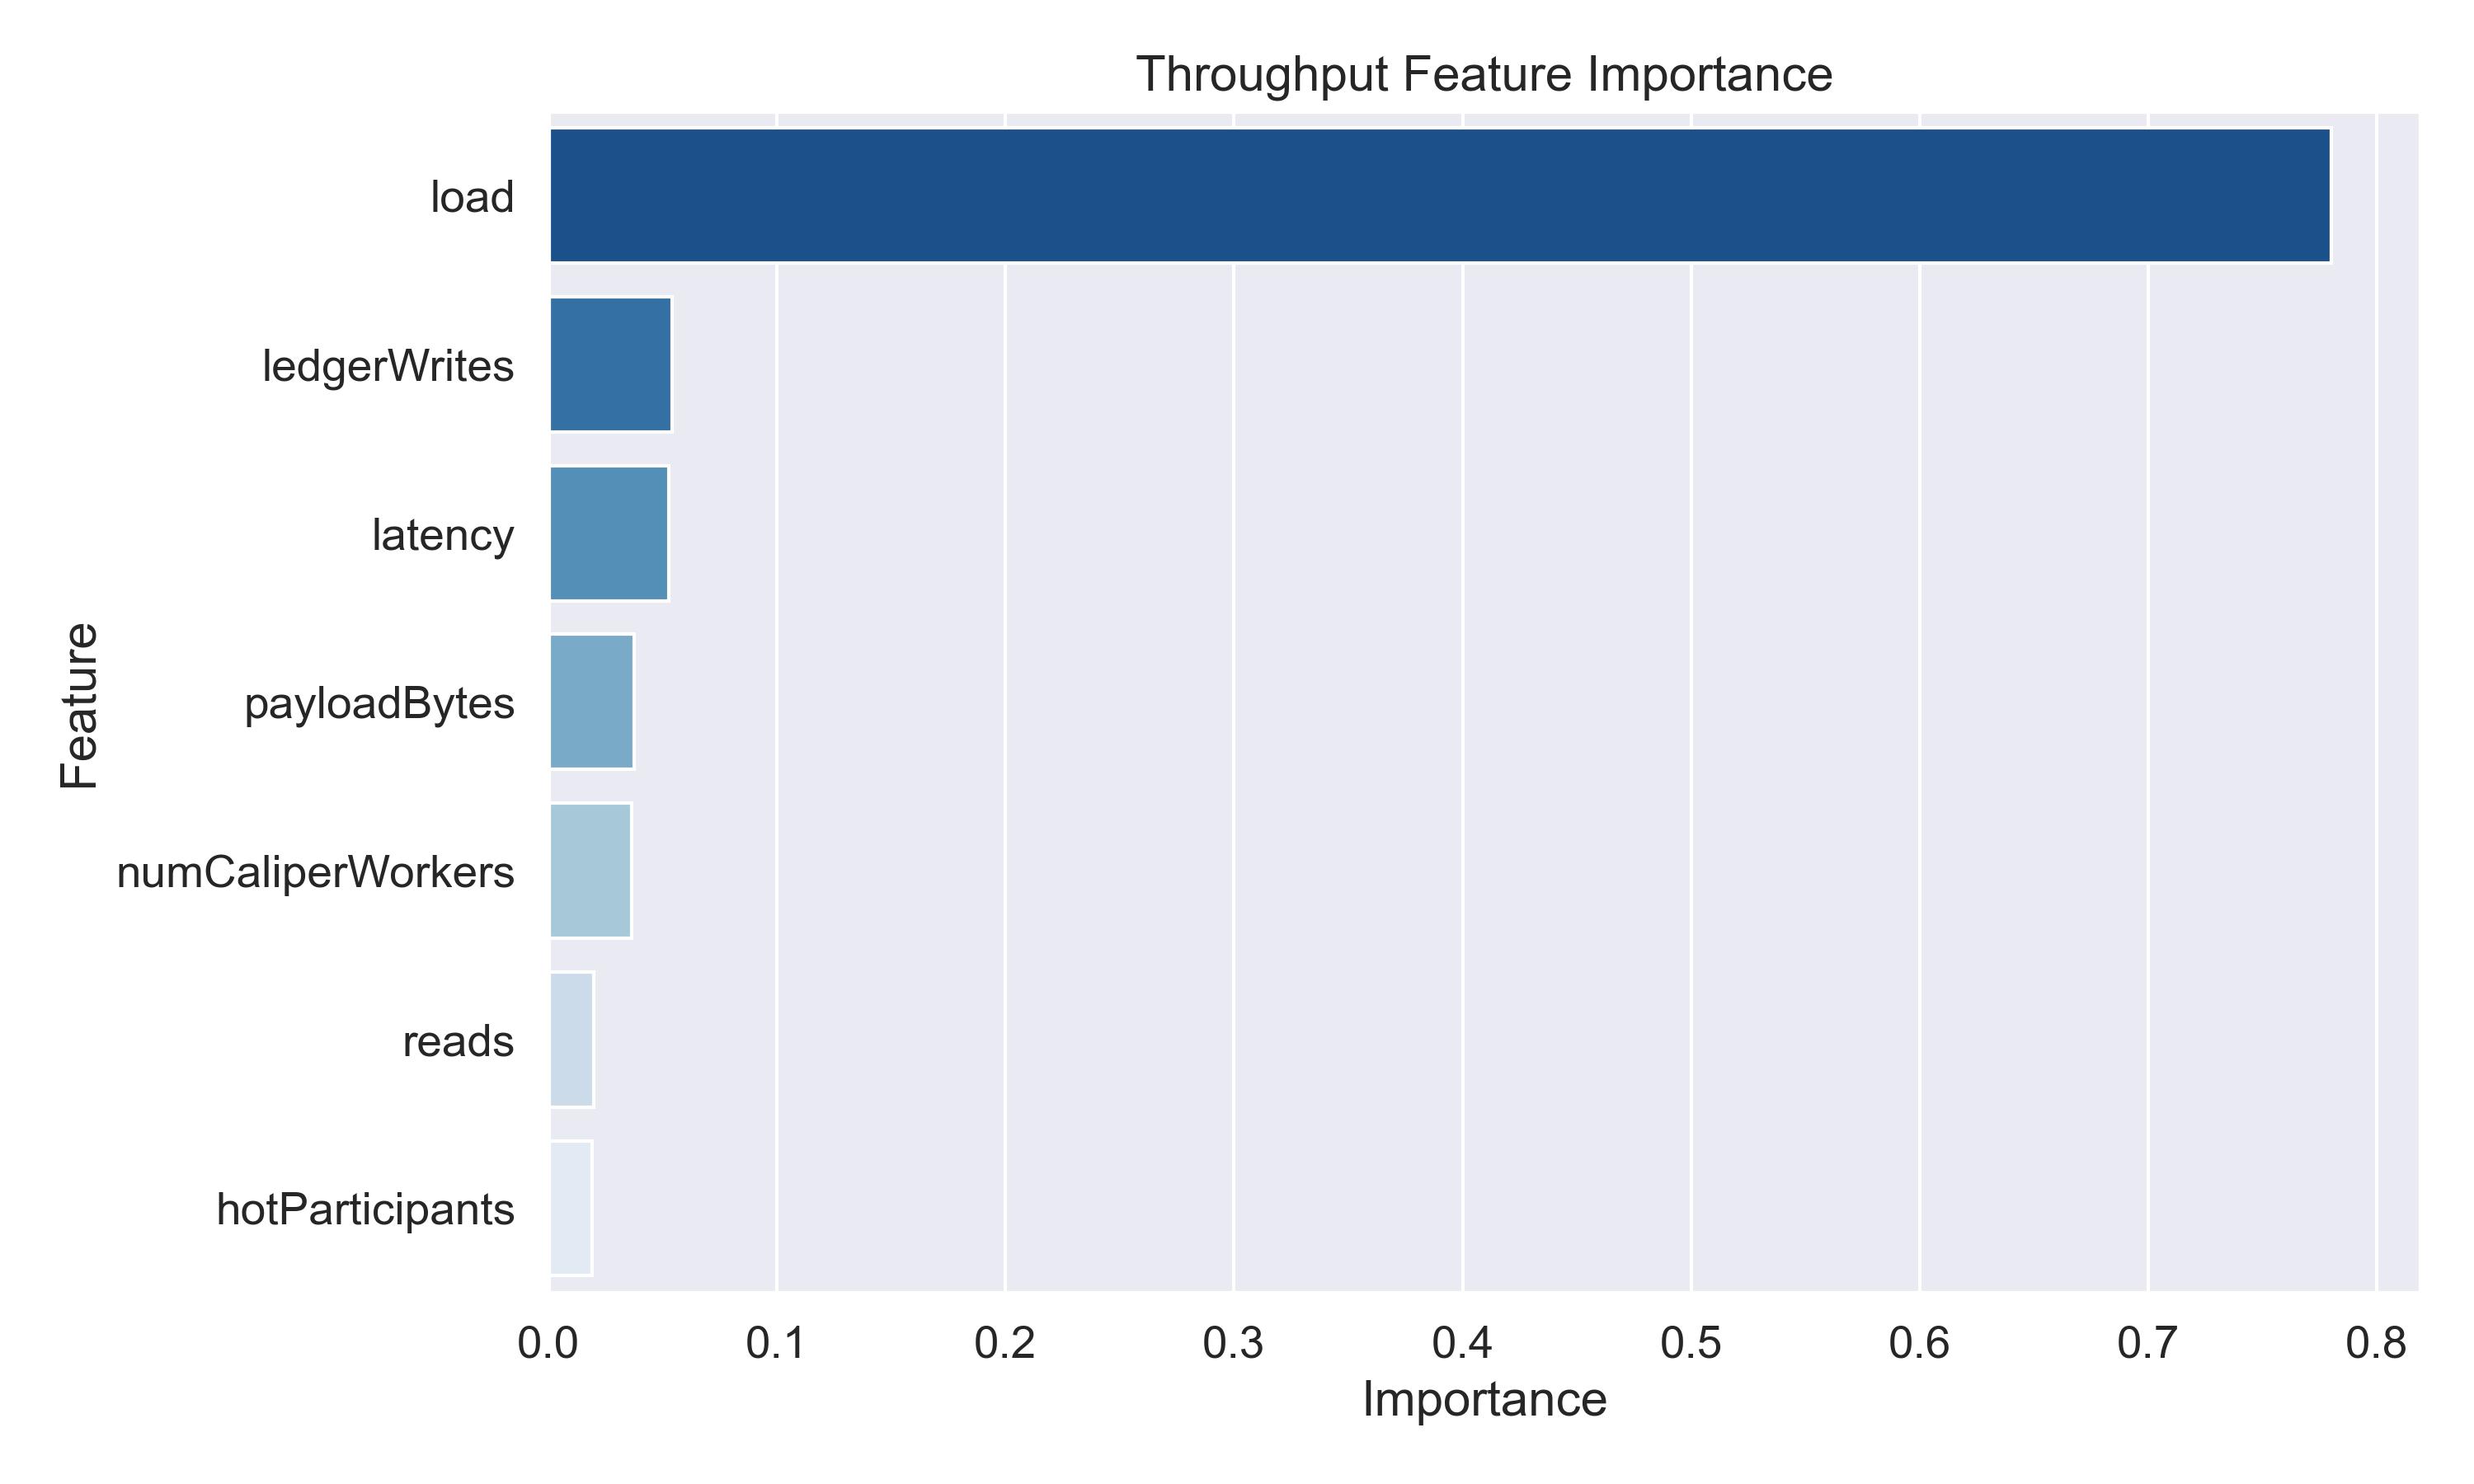
\includegraphics[width=0.8\textwidth]{Figure_11.png}
\caption{Random Forest Feature Importance ranking the dominant variables that constrain successful transaction throughput.}
\label{fig:throughput-feature-importance}
\end{figure}



\subsubsection{Failure Prediction and Feature Importance}
Table \ref{tab:failure_performance} presents the comparative predictive performance of each model for transaction failure rate.

\begin{table}[ht]
\centering
\caption{Comparative Predictive Performance (Target: Transaction Failure Rate)}
\label{tab:failure_performance}
\resizebox{0.8\columnwidth}{!}{%
\begin{tabular}{|l|c|c|c|}
\hline
\textbf{Machine Learning Model} & \textbf{$R^2$ Score} & \textbf{MAE} & \textbf{RMSE} \\
\hline
Linear Regression & 0.6680 & 0.169 & 0.224 \\
Gradient Boosting & 0.9057 & 0.0720 & 0.1077 \\
\textbf{Random Forest Regressor} & \textbf{0.9570} & \textbf{0.0368} & \textbf{0.0808} \\
\hline
\end{tabular}%
}
\end{table}

The Random Forest model yielded highly accurate predictive performance for failure rates, with results consistent with the empirical observations recorded during benchmarking. As illustrated in Figure \ref{fig:feature-importance}, the number of concurrent \textbf{Hot-Key Participants} emerged as the dominant failure predictor, accounting for 50.8\% of feature importance. This finding corroborates the empirical results: elevated participant density concentrates write operations onto a restricted set of shared ledger keys, amplifying MVCC read-write conflicts and raising the rejection rate substantially. \textbf{Payload Bytes} (20.5\%), \textbf{Transaction Load} (16.0\%) and \textbf{Network Latency} (8.7\%) ranked as the next most influential predictors. Collectively, these results indicate that transaction failure is not primarily a function of aggregate send rate, but is instead driven predominantly by the density of concurrent state contention, with payload and load acting as amplifying factors.

\begin{figure}[H]
\centering
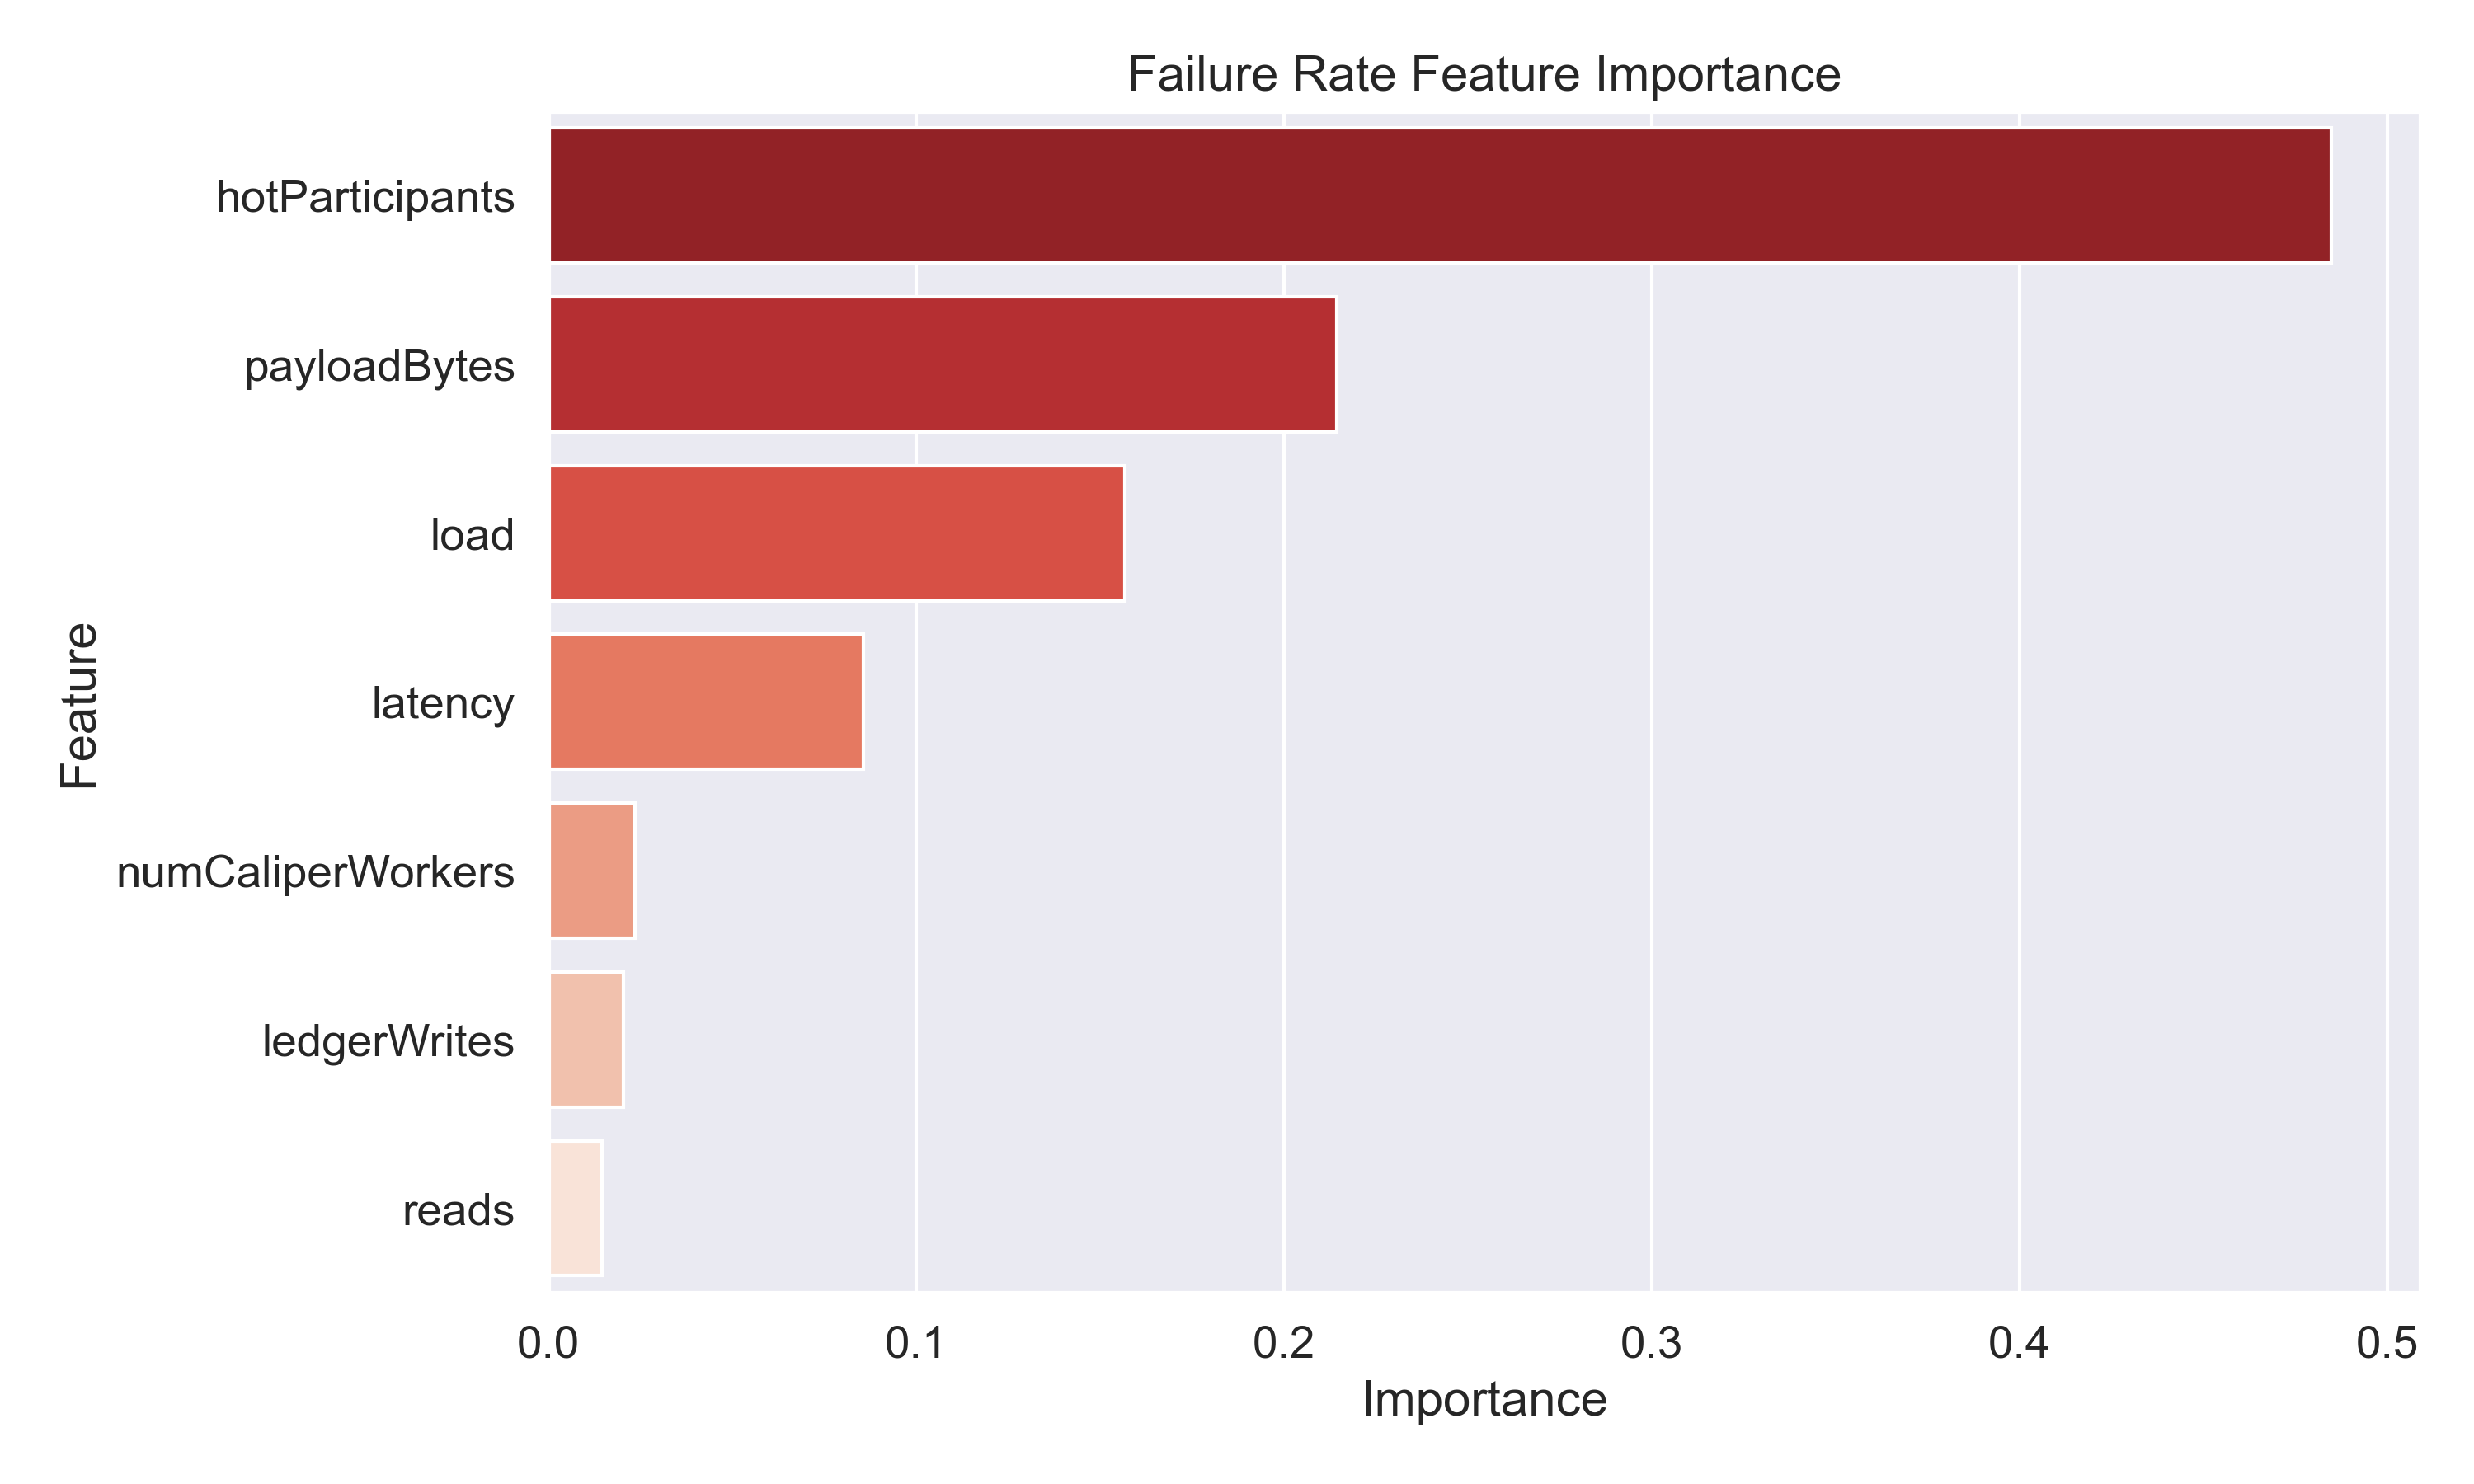
\includegraphics[width=0.8\textwidth]{Figure_12.png}
\caption{Random Forest Feature Importance ranking the distributed variables that trigger transaction failures.}
\label{fig:feature-importance}
\end{figure}



These findings indicate that mitigating transaction failure rates requires coordinated control of transaction concurrency rather than only increasing the offered load. In practice, transactions targeting the same hot keys can be scheduled or serialized to reduce simultaneous read-write conflicts, while the submitted TPS can be adjusted dynamically according to the observed contention level. Such workload-aware scheduling and TPS tuning directly address the primary source of MVCC contention observed throughout this study.

\section{Conclusion}

This study addressed a practical challenge in the deployment of permissioned blockchain systems for agricultural supply chains: the difficulty of anticipating and diagnosing transaction failures arising from Multi-Version Concurrency Control (MVCC) conflicts before they produce significant throughput degradation. A Hyperledger Fabric-based supply chain platform was used as an empirical testbed, and a supervised machine learning framework based on a Random Forest ensemble was developed to predict both transaction failure rates and throughput from a set of interpretable structural and operational features. The empirical benchmarking, conducted across 11 send-rate levels and a comprehensive participant matrix using Hyperledger Caliper, demonstrated that both transaction throughput and failure rates are strongly governed by the interaction between transaction load, concurrent participant density, ledger write complexity, and network latency. Empirically, transaction throughput scaled linearly with target load at lower send rates but saturated rapidly for functions with high per-transaction ledger write counts or when subjected to artificial network delay. Concurrently, chaincode functions that perform concurrent writes to shared ledger keys exhibited high failure rates, particularly under elevated transaction loads, as competing transactions converged on a narrow set of shared state records. As participant density increased, write operations were distributed across a wider set of independent ledger keys, substantially reducing conflict frequency. Transaction load further intensified contention by increasing the rate at which concurrent write conflicts were triggered within the same block generation window. Network latency compounded this effect by extending the endorsement and commit window, thereby increasing the probability that in-flight transactions would encounter stale state versions.

The predictive modelling results corroborated these observations. The Random Forest model identified the number of concurrent hot-key participants as the dominant driver of failure (50.8\%), followed by transaction payload (20.5\%) and transaction load (16.0\%). For throughput prediction, the raw transaction send rate accounted for the majority of predictive importance (81.1\%), with ledger write complexity and network latency contributing as secondary structural constraints. The model achieved $R^2$ scores of 0.9236 for throughput and 0.9570 for failure rate, confirming its suitability as a diagnostic instrument for pre-deployment performance assessment.

These findings demonstrate that mitigating MVCC failures in permissioned blockchain systems is not primarily a question of controlling transaction volume, but rather of managing the structural conditions under which concurrent write operations occur. Chaincode designs that distribute write targets across independent composite keys---rather than concentrating updates on shared state---represent the most effective architectural response to this challenge.

The primary objective of future work is the development of a \textbf{blockchain digital twin} that operationalises the predictive models developed in this study. The digital twin will maintain a real-time replica of the network state and, using the trained Random Forest model, continuously predict the expected failure rate and throughput for the current combination of transaction load, participant density, and network latency. Based on these predictions, the digital twin will act as an intelligent transaction scheduler: dynamically throttling submission rates when the predicted failure rate exceeds a defined threshold, redistributing load across participant roles to reduce hot-key contention, and deferring low-priority transactions during periods of high predicted conflict. This feedback loop will allow the system to self-regulate transaction execution and proactively prevent cascading MVCC failures in live production environments, rather than reacting to failures after they have occurred. Additional directions include extending and validating the framework in distributed multi-host deployments under wide-area network conditions.
\section*{Data availability}
	Data will be made available on request.
	
	\section*{Acknowledgements}
	This work was supported by \textbf{National Institute of Technology Calicut (NIT Calicut)}.
	
	\section*{Code Availability}
	The source code, configuration files, and benchmarking scripts used in this study are publicly available at:
	
	\url{https://github.com/dhanishjose123/predictive_benchmarking}
	
	\section*{Declaration of generative AI and AI-assisted technologies in the writing process}
	During the preparation of this work the author(s) used DeepL and ChatGPT in order to improve language and readability. After using these tools, the author(s) reviewed and edited the content as needed and take full responsibility for the content of the publication.
	
	\appendix
	

	
	
	\section*{CRediT authorship contribution statement}
Dhanish Jose: Writing - original draft, Writing - review \& editing, Validation, Methodology, Conceptualization.\\
Pradeepmon T G: Writing - review \& editing, Validation, Resources, Supervision.

\section*{Declaration of competing interest}
The authors declare that they have no known competing financial interests or personal relationships that could have appeared to influence the work reported in this paper.

\bibliography{references}
	% <-- REQUIRED line
	
\end{document}





